% BU ECE template for MS thesis and PhD dissertation.
%
%==========================================================================%
% MAIN PREAMBLE 
%==========================================================================%
\documentclass[12pt]{report}          % Single-sided printing for the library
%\documentclass[12pt,twoside]{report} % Double-sided printing
\usepackage[intlimits]{amsmath}
\usepackage{amsfonts,amssymb}
\DeclareSymbolFontAlphabet{\mathbb}{AMSb}
%\usepackage{natbib}
\usepackage{apalike}
%\usepackage{float}
%\usepackage[bf]{caption2}       
%\setcaptionmargin{0.5in}
\usepackage{fancyheadings,fancybox,ifthen}
\usepackage{bu_ece_thesis}
\usepackage{url}
\usepackage{lscape,afterpage}
\usepackage{xspace}
\usepackage{textcomp}

\usepackage{mathtools}
\usepackage{verbatim}
\usepackage{algorithm}
\usepackage{algorithmicx}
\usepackage[noend]{algpseudocode}
\usepackage{color}
\usepackage{colortbl}
\usepackage{subfig}
\usepackage{appendix}
\usepackage{undertilde}
\usepackage{lscape}

% code listings
\usepackage{listings}
\lstset{
	language=C++,
	numbers=left,
	numberstyle=\tiny,
	stepnumber=2, numbersep=5pt,
	basicstyle=\ttfamily\footnotesize,
	keywordstyle=\color{blue},
	commentstyle=\color{cblue},
	xleftmargin=\parindent,
	numbers=left,
	numberstyle=\tiny
}

\usepackage{multirow}

% colours
\definecolor{cblue}{rgb}{0.098,0.357,0.675}	

%==========================================================================%
%%% graphicx and pdf creation
\usepackage[]{graphicx}
%\usepackage{psfrag}
%\DeclareGraphicsExtensions{.eps}   % extension for included graphics
%\usepackage{thumbpdf}              % thumbnails for ps2pdf
%\usepackage[ps2pdf,                % hyper-references for ps2pdf
%bookmarks=true,%                   % generate bookmarks ...
%bookmarksnumbered=true,%           % ... with numbers
%hypertexnames=false,%              % needed for correct links to figures !!!
%breaklinks=true,%                  % breaks lines, but links are very small
%linkbordercolor={0 0 1},%          % blue frames around links
%pdfborder={0 0 112.0}]{hyperref}%  % border-width of frames 
%                                   % will be multiplied with 0.009 by ps2pdf
%\hypersetup{
%  pdfauthor   = {Joe Graduate <joe.graduate@bu.edu>},
%  pdftitle    = {dissertation.pdf},
%  pdfsubject  = {doctoral dissertations},
%  pdfkeywords = {mathematics, science, technology},
%  pdfcreator  = {LaTeX with hyperref package},
%  pdfproducer = {dvips + ps2pdf}
%}
%==========================================================================%
% customized commands can be placed here
%\newcommand{\figref}[1]{Figure~\ref{#1}}
%\newcommand{\chapref}[1]{Chapter~\ref{#1}}
%\newcommand{\latex}{\LaTeX\xspace}

% DEFINITIONS
\newcommand{\R}{\mathbb{R}}
\newcommand{\Z}{\mathbb{Z}}
\newcommand{\K}{\mathbb{K}}
\newcommand{\cpu}{\textsc{cpu}}
\newcommand{\gpu}{\textsc{gpu}}
\newcommand{\cuda}{\textsc{cuda}}
\newcommand{\mpi}{\textsc{mpi}}
\newcommand{\bem}{\textsc{bem}}
\newcommand{\bie}{\textsc{bie}}
\newcommand{\fmm}{\textsc{fmm}}
\newcommand{\fmmbem}{\fmm-\bem}
\newcommand{\aca}{\textsc{aca}}
\newcommand{\cpp}{\textsc{c++}}
\newcommand{\blas}{\textsc{blas}}
\newcommand{\sse}{\textsc{sse}}

% CURLY LETTERS
\newcommand{\bigO}{\mathcal{O}}
\renewcommand{\O}[1]{\mathcal{O}(#1)}

% FMM OPERATOR DEFINITIONS
%\newcommand{\ptop}{\textsc{p2p}}
%\newcommand{\ptom}{\textsc{p2m}}
%\newcommand{\mtom}{\textsc{m2m}}
%\newcommand{\mtop}{\textsc{m2p}}
%\newcommand{\mtol}{\textsc{m2l}}
%\newcommand{\ltol}{\textsc{l2l}}
%\newcommand{\ltop}{\textsc{l2p}}

\newcommand{\ptom}{\textsc{p}\texttwooldstyle\textsc{m}\xspace} % P2M
\newcommand{\ltop}{\textsc{l}\texttwooldstyle\textsc{p}\xspace} % L2P
\newcommand{\mtop}{\textsc{m}\texttwooldstyle\textsc{p}\xspace} % M2P
\newcommand{\mtom}{\textsc{m}\texttwooldstyle\textsc{m}\xspace} % M2M
\newcommand{\mtol}{\textsc{m}\texttwooldstyle\textsc{l}\xspace} % M2L
\newcommand{\ltol}{\textsc{l}\texttwooldstyle\textsc{l}\xspace}  % L2L
\newcommand{\ptop}{\textsc{p}\texttwooldstyle\textsc{p}\xspace} % P2P

% MISC THINGS
\newcommand{\ncrit}{N_{\text{CRIT}}}
\newcommand{\pmin}{p_{\text{min}}}
\newcommand{\tsolve}{t_{\text{solve}}}
\newcommand{\csr}{\textsc{csr}}
\newcommand{\nvidia}{\textsc{nvidia}}
\newcommand{\amg}{\textsc{amg}}

% SOLVER DEFINITIONS
\newcommand{\cg}{\textsc{cg}}
\newcommand{\gmres}{\textsc{gmres}}
\newcommand{\fgmres}{\textsc{fgmres}}
\newcommand{\bicgstab}{\textsc{bicgstab}}

% the text 'd' for integrals
\newcommand{\di}[1]{\text{d}#1}
% partial derivatives (frac)
\newcommand{\partiald}[2]{\frac{\partial #1}{\partial #2}}
% partial derivatives (inline)
\newcommand{\partialdi}[2]{\partial #1 / \partial #2}
% \hat{n}
\newcommand{\nhat}{\hat{n}}
% define a vector - undertilde
%\newcommand{\vect}[1]{\utilde{#1}}
% - bold
\newcommand{\vect}[1]{\mathbf{#1}}
% curly L
\renewcommand{\L}{\mathcal{L}}
% curly D
\newcommand{\D}{\mathcal{D}}
% sign
\newcommand{\sign}{\text{sign}}
% basis vectors
\newcommand{\e}{\vect{e}}
% dyadic product
\newcommand{\dyad}[2]{#1 \otimes #2}

%==========================================================================%

%==========================================================================%
% BEGIN
%==========================================================================%
\begin{document}

%\include{TODO}

% The preliminary pages
%!TEX root = ../thesis.tex

% This file contains all the necessary setup and commands to create
% the preliminary pages according to the buthesis.sty option.

\title{Fast multipole boundary element solutions with inexact Krylov iterations and relaxation strategies}

\author{Simon Layton}

% Type of document prepared for this degree:
%   1 = Master of Science thesis,
%   2 = Doctor of Philisophy dissertation.
%   3 = Master of Science thesis and Doctor of Philisophy dissertation.
\degree=2

\prevdegrees{B.Sc., University of Bristol, 2008 \\
M.S., Boston University, 2011}

\department{Department of Mechanical Engineering}

% Degree year is the year the diploma is expected, and defense year is
% the year the dissertation is written up and defended. Often, these
% will be the same, except for January graduation, when your defense
% will be in the fall of year X, and your graduation will be in
% January of year X+1
\defenseyear{2013}
\degreeyear{2013}

% For each reader, specify appropriate label {First, second, third},
% then name, then title. Warning: If you have more than five readers
% you are out of luck, because it will overflow to a new page.
% Sometimes you may wish to put part of the title in with the name
\reader{First}{Lorena Barba, PhD}
{Assistant Professor of Mechanical Engineering}
\reader{Second}{Sheryl Grace, PhD}{Associate Professor of Mechanical Engineering}
\reader{Third}{Paul Barbone, PhD}{Associate Professor of Mechanical Engineering}
\reader{Fourth}{Emily Ryan, PhD}{Assistant Professor of Mechanical Engineering}

% The Major Professor is the same as the first reader, but must be
% specified again for the abstract page
\majorprof{Lorena A. Barba, PhD}{\mbox{Department of Mechanical Engineering}}

%                       PRELIMINARY PAGES
% According to the BU guide the preliminary pages consist of:
% title, copyright (optional), approval,  acknowledgments (opt.),
% abstract, preface (opt.), Table of contents, List of tables (if
% any), List of illustrations (if any). The \tableofcontents,
% \listoffigures, and \listoftables commands can be used in the
% appropriate places. For other things like preface, do it manually
% with something like \newpage\section*{Preface}.

% This is an additional page (do not hand it in at the library) to print
% boxed-in title, author and degree statement so that they are visible through
% the opening in BU covers used for reports. This makes a nicely bound copy.
\buecethesistitleboxpage

% Make the titlepage based on the above information.  If you need
% something special and can't use the standard form, you can specify
% the exact text of the titlepage yourself.  Put it in a titlepage
% environment and leave blank lines where you want vertical space.
% The spaces will be adjusted to fill the entire page.
\maketitle
\cleardoublepage

% The copyright page is blank except for the notice at the bottom. You
% must provide your name in capitals.
\copyrightpage
\cleardoublepage

% Now include the approval page based on the readers information
\approvalpage
\cleardoublepage

% Here goes your favorite quote.
\newpage
\thispagestyle{empty}
%!TEX root = ../thesis.tex

\phantom{.}
\vspace{4in}

\begin{singlespace}
\begin{quote}
  %\textit{Facilis descensus Averni;}\\
  %\textit{Noctes atque dies patet atri janua Ditis;}\\*
  %\textit{Sed revocare gradum, superasque evadere ad auras,}\\
  %\textit{Hoc opus, hic labor est.}\hfill{Virgil (from Don's thesis!)}
  \textit{To my parents Dennis and Wendy, and my beloved fianc\'ee Elizabeth}
\end{quote}
\end{singlespace}

% \vspace{0.7in}
%
% \noindent
% [The descent to Avernus is easy; the gate of Pluto stands open night
% and day; but to retrace one's steps and return to the upper air, that
% is the toil, that the difficulty.]

\cleardoublepage

% The acknowledgment page should go here. Use something like
% \newpage\section*{Acknowledgments} followed by your text.
\newpage
\section*{\centerline{Acknowledgments}}
%!TEX root = ../thesis.tex

%I would like to thank Jonathan Polimeni for cleaning up all these old
%LaTeX style files and templates so that I didn't have to use Word to
%write up this document. Also, I would like to thank all the CV/CNS lab
%graduates for their contributions and tweaks to this organizational
%scheme over the years (after many dissapointing interactions with
%Martha Wellman).
%
%This brings me to thank Martha Wellman of CAS and Brendon McDermot of
%Mugar library who together uphold the stylistic and aesthetic
%conventions that have been implemented in this LaTeX manuscript. Also
%Sister Mary Virginia, the Thesis/dissertation coordinator of Mugar
%Library, deserves some thanks as well.
%
%Finally, I would like to thank Stephen Gildea, for the MIT sytle file
%off which this current version is based, and Paolo Gaudiano for
%porting the MIT style to one compatible for BU.

% [[[ LORENA ]]]
I would like to express wholehearted gratitude to my academic advisor over the last 6 years, Prof. Barba for her support and guidance throughout my studies in two universities, 3 degrees and 2 continents. In particular I would like to thank her for the belief she showed in me by bringing me from Bristol to Boston University in order to continue my studies. I deeply appreciate the freedom I have been given in my research, along with the invaluable advice and support that has been key to my successes.

% [[[ COMMITTEE ]]]
I would also like to thank the members of my committee, Professors Paul Barbone, Sheryl Grace and Emily Ryan for their time and insights during these final months of my studies.

% [[[ GROUP ]]]
With the contributions, ideas and friendship of Christopher Cooper, Anush Krishnan, Brent Parham and Olivier Mesnard in Prof. Barba's research group, the time I have spent here has flown by, and they have always been willing to help in any way necessary, be it debugging code, reading papers or spending time relaxing away from the office. Special thanks must also go to Rio Yokota, who was always available for advice on coding, {\fmm} or any other subject.

% [[[ OTHERS ]]]
I also take this opportunity to thank those who have helped and funded me through my time at Boston University -- Dan Kamalic for his patience in helping me with the use of his compute clusters. My continued funding has been greatly appreciated, and I would like to thank Boston University, the Massachusetts Green High-Performance Computing Center (MGHPCC), National Science Foundation (NSF) and the Office of Naval Research (ONR) for their contributions. 

% [[[ PARENTS ]]]
I would like to thank my fianc\'ee, Elizabeth Matos for the love and support she has shown me, both pulling me through the last parts of my studies, and giving me an incredible future to look forward to. Finally, I wish to show my appreciation for my parents, Dennis and Wendy Layton for their unending and unconditional encouragement and belief, for always being there for me, and for not begrudging me this time far away from them in Boston. 

\cleardoublepage

% The abstractpage environment sets up everything on the page except
% the text itself.  The title and other header material are put at the
% top of the page, and the supervisors are listed at the bottom.  A
% new page is begun both before and after.  Of course, an abstract may
% be more than one page itself.  If you need more control over the
% format of the page, you can use the abstract environment, which puts
% the word "Abstract" at the beginning and single spaces its text.

\begin{abstractpage}
%!TEX root = ../thesis.tex

Boundary element methods (\bem) have been used for years to solve a multitude of engineering problems, ranging from Bioelectrostatics, to fluid flows over micro-electromechanical devices and deformations of cell membranes. Only requiring the discretization of a surface into panels rather than the entire domain, they effectively reduce the dimensionality of a problem by one.

This reduction in dimensionality nevertheless comes at a cost. {\bem} requires the solution of a large, dense linear system with each matrix element formed of an integral between two panels, often performed used an iterative solver based on Krylov subspace methods. This requires the repeated calculation of a matrix vector product that can be approximated using a hierarchical approximation known as the fast multipole method (\fmm). While adding complexity, this reduces order of the time-to-solution from $\O{cN^{2}}$ to $\O{cN}$, where $c$ is some function of the condition number of the dense matrix.

This thesis obtains algorithmic speedups for the solutions of {\fmmbem} systems by applying the mathematical theory behind inexact matrix-vector products to our solver, implementing a relaxation scheme to control the error incurred by the {\fmm} in order to minimize the total time-to-solution. The theory is extensively verified for both Laplace equation and Stokes flow problems, with an investigation to determine how further problems may benefit from the addition of a relaxed solver. We also present experiments for the Stokes flow around both single and multiple red blood cells, an area of ongoing research, showing good speedups that would be applicable for any other code that chose to implement a similar relaxed solver. All of these results are obtained with an easy-to-use, extensible and open-source {\fmmbem} code.


% Engineering problems become ever larger, and we continually look for better ways to simulate them. Boundary elements (BEM) are a integral formulation over a surface, only requiring discretization of the surface rather than the entire domain, effectively reducing the dimensionality of a problem from a volume to a surface in 3D.

% BEM requires the iterative solution of a large dense linear system, in our case solved using GMRES, a Krylov subspace method that uses repeated matrix-vector products. These are accelerated using a fast multipole method or treecode, reducing the time to solution from O(N^2) to O(N).

% We apply the mathematical theory behind inexact matrix products and relaxation to our BEM solver, utilizing the ability of fast multipole methods to control error in order to minimize time to solution. This is combined with preconditioners and inner-outer solvers, and extensively tested in a new, extensible computational framework.

\end{abstractpage}
\cleardoublepage

% Now you can include a preface. Again, use something like
% \newpage\section*{Preface} followed by your text

% Table of contents comes after preface
\tableofcontents
\cleardoublepage

% If you have tables, uncomment the following line
%\listoftables
%\cleardoublepage

% If you have figures, uncomment the following line
\newpage
\listoffigures
\cleardoublepage

% List of Abbrevs is NOT optional (Martha Wellman likes all abbrevs listed)
\chapter*{List of Abbreviations}
\begin{center}
  \begin{tabular}{lll}
    \hspace*{2em} & \hspace*{1in} & \hspace*{4.5in} \\
    BEM  & \dotfill & Boundary Element Method \\
    FMM  & \dotfill & Fast Multipole Method \\
    GMRES & \dotfill & Generalized minimal residual \\
    FGMRES & \dotfill & Flexible generalized minimal residual \\
    BLAS & \dotfill & Basic Linear Algebra Subroutines \\
    P2P & \dotfill & Particle-to-Particle \\
    P2M & \dotfill & Particle-to-Multipole \\
    M2M & \dotfill & Multipole-to-Multipole \\
    M2L & \dotfill & Multipole-to-Local \\
    L2L & \dotfill & Local-to-Local \\
    L2P & \dotfill & Local-to-Particle
  \end{tabular}
\end{center}
\cleardoublepage

% List of algorithms
\newpage
\listofalgorithms
\cleardoublepage

% END OF THE PRELIMINARY PAGES

\newpage
\endofprelim
        
\cleardoublepage

% -------------------------------------
% CHAPTER 1: INTRODUCTION
% -------------------------------------
%!TEX root = ../thesis.tex

\chapter{Introduction}
\label{chapter:Introduction}
\thispagestyle{myheadings}

\section{Introduction}\label{sec:introduction}

As engineering problems and simulations become ever larger, and we continually look for new and better ways to simulate them, maximizing both the size of problem we can compute, and the speed at which we can obtain an answer. Problems become more complex as they move from 2 dimensional approximations to 3 dimensional simulations, leading to the natural question of how to both reduce the amount of work that has to be done, and how efficiently we can do it.

% BEM introduced
Boundary element methods (\bem) were introduced in the 1960s (standard introductory texts however, came later \cite{BrebbiaDominguez1992}) for a subset of problems, reducing the computational domain from the entirety of the needed physical space (volume / area) to the boundary of the region of interest (surface / curve), discretized into panels. The reduction in dimensionality changes a problem from $3$ or $2$ dimensions, to one dimension lower.

{\bem}'s major downside is that it requires the solution of a dense system of linear equations, $A\vect{x} = \vect{b}$, where $A \in \R^{N\times N}$ and $N$ is the number of discretized panels. Due to the density of $A$, in the best case with an iterative solver, work and memory requirements for this solution scale as the size of the matrix, or in asymptotic notation, $\bigO(cN^{2})$ time, where $c$ is a function of the condition number of $A$, while a traditional dense solve, such as Gauss elimination would require $\O{N^{3}}$ time. This scaling is in comparison to (for instance) finite element, volume or difference codes, which still require the solution of a linear system, but in their case $A$ is sparse, allowing solutions to be found in $\bigO(cN)$ time, where $N$ is now the number of degrees of freedom used, $c$ is again a function of the condition number of $A$, and in general this $N$ is significantly larger than the $N$ for {\bem} problems. The $\O{cN^{2}}$ scaling causes {\bem} to become unusable for larger and more complex problems.

% FMM introduced
Initially introduced to quickly calculate potential fields for particle methods, Treecodes were developed in the late 1980s \cite{BarnesHut1986}. The computational domain is hierarchically split into near and far-field components, then far-field interactions are approximated with multipole expansions. These multipole expansions are faster than evaluating individual particles, but they are only convergent for distant targets. The near-field is still computed directly, preserving accuracy. Importantly, this splitting and approximation reduces the time taken to evaluate the interactions between $N$ particles to $\O{N\log N}$. The fast multipole method ({\fmm}) was introduced soon after as a further improvement, modifying the far-field evaluation by translating multipoles into local expansions \cite{greengard1987} that are accurate close to the expansion center and evaluating them instead of directly using the multipoles. This translation further reduced the complexity to the optimal $\bigO(N)$. The {\fmm} was later named as one of the top 10 scientific algorithms of the 20th century \cite{DongarraSulli2000}.

% FMM-BEM
Several years later, the potential of using fast methods to accelerate {\bem} was realized for the Laplace\cite{Nabors94} and Stokes \cite{gomez1997} equations. By using a fast method within an iterative solution of the {\bem} linear system, the scaling was reduced from $\bigO(N^{2})$ to $\bigO(cN)$, making larger simulations feasible. While this modification adds complexity to the {\bem}, it allows users to perform much larger experiments, putting them on a more level playing field to more traditional computational methods, such as finite elements.

% KRYLOV & INEXACT MATVEC
Parallel to the development of {\bem} and {\fmm}, the linear algebra community was working on iterative solvers. The widely used {\gmres} algorithm \cite{SaadSchultz1986}, published in 1986, iteratively solves $Ax = b$ for a general $A \in \R^{N\times N}$, by generating a Krylov subspace through repeated matrix-vector multiplication, and finding the vector $x_{k}$ within this space that minimises $||Ax_{k}-b||$. The cost of this method scales as the cost of the product of computing the matrix-vector products and a function of the condition number of $A$, denoted as $c$, thus when used in a standard {\bem} the cost would be $\O{cN^{2}}$, while for the {\fmm}-{\bem}, the cost is $\bigO(cN)$.

% RELAXATION (INEXACT MATVEC) AND PRECONDITIONERS
Where the iterative solution of $Ax = b$ dominates solution time, methods have been proposed to reduce both the number of iterations needed, and the cost of each of those iterations. In general the convergence rate of a solver depends on the condition number of $A$. The most commonly used way to reduce the condition number is to use a preconditioner. These can be as simple as using the inverse of the diagonal of $A$, or as complex as performing a complete additional linear solve. 

The theory behind inexact matrix-vector products in the context of Krylov solvers \cite{simonciniszyld2003,bourasfraysse2005} was initially developed to explain experimental results where error was introduced into the matvec within a solver, yet the correct results were obtained with no loss of convergence. While this concept is well developed within the linear algebra community, there is no work that we are aware of on applying the theory to {\fmmbem} problems by \emph{relaxing} the accuracy of the {\fmm}-accelerated matvecs.

%To reduce the cost of an iteration, relaxation methods were introduced \cite{simonciniszyld2003,bourasfraysse2005}, relying on the ability to compute an \emph{inexact} matrix-vector product at lower cost than the exact product. While the theory is well-developed within the math community \cite{simonciniszyld2003,vandeneshofsleijpen2004}, there is no  work on applying that theory to {\fmmbem} problems. 

\section{Objective}\label{sec:objective}

This thesis aims to apply current inexact Krylov and relaxation method theory to the field of {\fmmbem} problems. To achieve this goal we first perform extensive verification tests on a comparatively simple test problem, before using this problem to thoroughly examine the performance characteristics of utilizing a relaxation method. These experiments allow us to provide guidelines to help identify more potential problems for the use of a relaxed solver. Next, we verify the relaxed solver on a more complicated example, then use a problem within the engineering field to illustrate the practical performance gains of relaxation methods.

\section{Present Contribution}\label{sec:present_contribution}

This study presents the following work

\begin{enumerate}
\item An extendible, easy-to-use modern code for {\fmm}, {\bem} and {\fmmbem} problems, complete with both exact and inexact solvers, simple preconditioners, relaxation schemes and the ability to solve multiple kinds of problems including the Laplace and Stokes equations. This includes the first fully open-source {\fmmbem} solver for the Stokes equation.

\item Use and verification of inexact Krylov solver theory with {\fmmbem} problems for the first time. This study also provides guidelines for identifying problems that might benefit from relaxation schemes. %includes extensive performance testing, and provides a significant addition to the {\fmmbem} community.

\item Extensive performance testing for both simple (Laplace) and more complex (Stokes) {\bem} problems, including the field of blood flow, showing speedups from the use of a relaxed solver.

\end{enumerate}

\section{Contents of the Thesis}\label{sec:contents_of_thesis}

This thesis is organized as follows. In chapter \ref{chapter:background}, some background is introduced for the component methods of this research work: {\bem}, {\fmm}, Krylov iterative solvers and inexact matrix-vector products. Next, in chapter \ref{chapter:methods}, we discuss the implemented numerical methods that have been used in the current work, concentrating on numerical integrals along with a relaxation scheme and preconditioners. Chapter \ref{chapter:fmm_implementation} discusses some implementation-specific details for the {\fmm} used in this thesis. We then use the techniques from chapters \ref{chapter:methods} and \ref{chapter:fmm_implementation} to problems involving the Laplace equation in chapter \ref{chapter:laplace_bem}, presenting convergence tests, relaxation verification and performance results. Using a Laplace problem we experiment further with the parameter space of relaxation, obtaining some general rules by which one can determine whether a given problem will benefit from a relaxed solver. In chapter \ref{chapter:stokes} these rules are applied to a more significant problem, Stokes flow. Experiments demonstrate both convergence of the method for this new equation and speedups with the relaxed solver. The final results-based section, chapter \ref{chapter:rbc}, explores the field of blood flow using the solver from chapter \ref{chapter:stokes} to explore the performance of our relaxed solver for this more complex and relevant engineering problem. Finally in chapter \ref{chapter:conclusions}, we discuss the expected impact of our completed work, along with the next steps that could be taken.

%%%%%%% OLD %%%
%A major part of this work explores the use of these relaxation schemes for that context, namely controlling the accuracy of the {\fmm}-accelerated matrix-vector product to accelerate {\gmres} solutions.
%
%This research work presents the use of an {\fmm}-accelerated {\bem} as a platform to explore, implement and design a fast, efficient solver for engineering problems. We use the combination of inexact matrix-vector products, relaxation strategies and {\fmm}-specific preconditioners to minimise the time needed to solve research problems.
%
%This work will explore the space of inexact Krylov solvers with and without preconditioners for problems solved with {\fmmbem}. While there exists some isolated work involving inner-outer {\gmres} solvers \cite{Chailletetal2011}, there is nothing beyond a notice of intention to investigate relaxation schemes applied to inexact matrix-vector products with fast methods \cite{raykarduraiswami2005}. We take this gap in knowledge, and perform both an investigation of the the theory as it applies to {\fmmbem}, and systematic testing with a variety of sample problems from a number of different topics. This investigation will explore the combinations of methods and parameters needed in order to minimize the time-to-solution of our problems, and provide guidelines as to potential effect in other situations. Further, all these experiments will be performed using a newly-written, open-source {\fmmbem} code.


\cleardoublepage

% -------------------------------------
% CHAPTER 2: BACKGROUND
% -------------------------------------
%!TEX root = ../thesis.tex

\chapter{Background}
\label{chapter:background}
\thispagestyle{myheadings}

% set this to the location of the figures for this chapter. it may
% also want to be ../Figures/2_Body/ or something. make sure that
% it has a trailing directory separator (i.e., '/')!
\graphicspath{{./Background/}}

%%%%% BEM
\section{Boundary Element Methods (BEM)}\label{sec:bem}

The boundary element method ({\bem}) is based around a technique to solve linear partial differential equations by formulating them as boundary integrals. This formulation requires that only the surface of a body of interest (such as an object in a medium) be discretized, and the solution is obtained on that surface. As a post-processing step, this solution can then be computed both inside and outside the body. The lower discretization requirement is an advantage over traditional grid-based methods that require the entire domain to be meshed. Furthermore, regardless of infinite or bounded domains, the solution process and discretization is exactly the same.

For example, we show the boundary integral form of the Laplace equation, $\nabla^{2}\phi = 0$ --- this will be derived much later in \S\ref{sec:bem_derivation}, but for now it is useful to see the form of the equation, where $G=1/4\pi r$ is the free-space Green's function for the Laplace equation.

\begin{equation}\label{eqn:bem_background_full}
	\frac{1}{2}\phi + \int_{\Gamma} \phi\partiald{G}{\nhat}\;\di{\Gamma} = \int_{\Gamma}\partiald{\phi}{\nhat}G\;\di{\Gamma}.
\end{equation}

We can see that all terms involved are now only on the boundary, $\Gamma$, and when we eventually form a linear equation, the unknowns will be boundary values of $\phi$ and $\partialdi{\phi}{\nhat}$.

The exact manner in which we choose to solve equation (\ref{eqn:bem_background_full}) can  now be discussed. First, $\Gamma$ is dicretized into \emph{panels}. Two pieces of nomenclature are now introduced -- we integrate over a \emph{source panel}, $j$ with respect to a \emph{target}, $i$, that can be a single point in space or a panel, depending on the formulation of {\bem} used. The 2 main families of methods for {\bem}, are \emph{collocation} and \emph{Galerkin} formulations. Collocation explicitly enforces equation (\ref{eqn:bem_background_full}) at a discrete set of points, $\vect{x}_i$, generally the centers of the target elements. By contrast, Galerkin formulations enforce the solution in a weighted average sense over an element, $\Gamma_i$. This is done by multiplying the function over the target panel with a test / shape basis function and performing an additional integral over the panel. Collocation {\bem} can be obtained from a Galerkin formulation by choosing a Dirac delta function as the test function.

Finally, {\bem} can use many different types of panel, each giving different convergence and error properties. We now describe two of the most commonly used panel types, \emph{constant} and \emph{linear}. \cite{BrebbiaDominguez1992}

\begin{enumerate}
\item \emph{Constant} -- Values (such as $\phi$ and $\partialdi{\phi}{\nhat}$) are considered to be constant across the entirety of the element. This is the most basic method, and allows the surface integrals encountered in {\bem} to be simplified greatly. For example, the integral $\int_{\Gamma} \phi\partialdi{G}{\nhat}\;\di{\Gamma}$ from equation (\ref{eqn:bem_background_full}) would be calculated as $\phi\int_{\Gamma}\partialdi{G}{\nhat}\;\di{\Gamma}$, as the value of $\phi$ is unchanging across the panel. % This method results in a linear system of $N$ variables, where $N$ is the number of panels.

\item \emph{Linear} -- Values vary linearly across the panel. More complex than constant elements, values must be calculated at every vertex of every panel in the domain, resulting in a larger linear system. The trade-off however, is that fewer panels should be needed to obtain the same quality of results as constant elements. 
\end{enumerate}

There are many more types of panels that can be used for {\bem}, varying in both the geometric sense, being curved or flat, and in terms of the distribution of values over the panel, such as the constant and linear distributions described above.

In this work, we use a collocation method with constant panels for all experiments, in keeping with   {\fmmbem} studies such as \cite{Liu2009} --- the extension of {\fmmbem} to linear elements is rare in the literature, and does not appear to be a fully-developed field. %, and all experiments will be performed using this style of panel.

%For an example, we look at the Laplace equation, $\nabla^{2}\phi = 0$ on a surface, $\Gamma$. We assume the domain can be split arbitrarily into $\Gamma_{1}$ and $\Gamma_{2}$, such that $\Gamma = \Gamma_{1} \cup \Gamma_{2}$ and $\Gamma_{1} \cap \Gamma_{2} = \emptyset$. Further, we know $\phi = \bar{\phi}$ on $\Gamma_{1}$ and $\partialdi{\phi}{\hat{n}} = \partialdi{\bar{\phi}}{\hat{n}}$ throughout the domain.
%
%We start with a weighted integral equation, with a test function $w$ and applying the Green-Gauss theorem twice to get:
%
%\begin{equation}\label{eqn:bem_1}
%	0 = \int_{\Gamma}\partiald{\phi}{\nhat}w\;\di{\Gamma} - \int_{\Gamma}\phi\partiald{w}{\nhat}\;\di{\Gamma} + \int_{\Omega}\phi\nabla^{2}w\;\di{\Omega}.
%\end{equation}
%
%We use the fundamental solution to the Laplace equation, $G$ as our test function, and the identity $\nabla^{2}G = -\delta$, turning the last term of \ref{eqn:bem_1}:
%
%\begin{equation}\label{eqn:bem_2}
%	\int_{\Omega}\phi\nabla^{2}w\;\di{\Omega} = -\phi.
%\end{equation}
%
%Choosing to solve for values of $\phi$ at the center of our discretized panels, we get a final integral equation of:
%
%\begin{equation}\label{eqn:bem_3}
%	\frac{1}{2}\phi_{i} - \int_{\Gamma} \phi\partiald{G}{\hat{n}}\;\di{\Gamma}' = \int_{\Gamma}\partiald{\phi}{\hat{n}} G\;\di{\Gamma}',
%\end{equation}

We discretize equation (\ref{eqn:bem_background_full}) by exchanging integrals over $\Gamma$ to sums over $N$ discretized panels, $\Gamma_j$ and take advantage of constant panels by moving the specified values, $\phi_j$ and $\partialdi{\phi}{\nhat}$ outside the surface integrals to get equation (\ref{eqn:bem_4}).

\begin{equation}\label{eqn:bem_4}
	\frac{1}{2}\phi_{i} - \sum_{j=1}^{N} \phi_j\int_{\Gamma_{j}}\partiald{G_{ij}}{\hat{n}} \;\di{\Gamma'} = \sum_{j=1}^{N} \partiald{\phi_{j}}{\hat{n}_j}\int_{\Gamma_{j}}G_{ij}\;\di{\Gamma'}
\end{equation}

From this form, solving for $\phi$ with a set $\partialdi{\phi}{\hat{n}}$ is known as a \emph{second-kind} equation, and solving for $\partialdi{\phi}{\hat{n}}$ for set $\phi$ is a \emph{first-kind} equation.

Given either $\phi$ or $\partialdi{\phi}{\hat{n}}$ for each panel in equation (\ref{eqn:bem_4}) we assemble the dense linear system

\begin{equation}
	A\vect{x} = \vect{b},
\end{equation}

\noindent
where for constant elements, $A_{ij}$ is either $\int_{\Gamma_{j}} \partialdi{G_{ij}}{\hat{n}}\;\di{\Gamma'}$ or $\int_{\Gamma_{j}}G_{ij}\;\di{\Gamma'}$ depending on whether $\phi$ or $\partialdi{\phi}{\hat{n}}$ respectively is known on panel $j$.

The techniques used for solving this form of equation quickly will be described throughout the next chapters of this thesis, including the evaluations of the different integrals, in \S\ref{subsec:numerical_integration}. However, it is useful to note at this point that for target points far away from a source panel we can approximate the surface integrals using Gauss quadrature, turning them into a simple repeated evaluation of $G$ or $\partialdi{G}{\nhat}$. The influence of all panels at a chosen target can then be thought of as an $N$-body sum.


% The techniques for the evaluation of these integrals will be described in \S\ref{subsec:numerical_integration}, but for now we merely state that for source panels a large distance from the target, we can use a summation over points contained within the source panel as an approximation to the integral.

%These integrals are evaluated using either Gaussian quadrature when panels are far away, or analytical / semi-analytics integrals when close together. This means we approximate our integrals using:

%\begin{equation}
%	\int_{\Gamma_{j}} f(x_{i},x_{j})\;\di{\Gamma'} = \sum_{k} A_j\cdot w_k\cdot f(x_{i},x_{k}).
%\end{equation}

%Thus, whenever we have the pattern in algorithm \ref{alg:sum_sources1}, we can replace it with algorithm \ref{alg:sum_sources2} where $\text{OP}$ is the function to be integrated. This conversion will allow us to accelerate our {\bem} using fast methods, described in the next section.


%\begin{algorithm}[h]
%	\caption{Loop over sources}
%	\label{alg:sum_sources1}	
%	\begin{algorithmic}
%	\Require sources, $j$
%	\For{all sources, $j$}
%		\Call{op}{$j$, ...}
%	\EndFor
%	
%	\end{algorithmic}
%\end{algorithm}
%
%\begin{algorithm}
%	\caption{Loop over Gauss quadrature points}
%	\label{alg:sum_sources2}
%	
%	\begin{algorithmic}
%	\Require sources, $j$
%	\For{all sources, $j$}
%		\For{points within panel $j$, $k$}
%			\State \Call{op}{$k$, ...}
%		\EndFor
%	\EndFor
%	
%	\end{algorithmic}
%\end{algorithm}

%%%%% KRYLOV METHODS
\section{Krylov Subspace Methods}\label{sec:krylov}

In many applications, including {\bem}, it is not feasible to solve the linear system $Ax = b$ in a direct fashion, due to either time or memory constraints. In these situations, iterative solvers are used, many of which (including conjugate gradient ({\cg}) and generalized minimal residual ({\gmres})) are based on Krylov subspaces. A Krylov subspace is a linear subspace which is spanned by the images of $b$ under powers of $A$. An \emph{order-$r$} subspace is comprised of the first $r$ images, denoted by:

\begin{equation}
	K_{r}(A,b) = \text{span}\{ b, Ab, A^{2}b, ..., A^{r-1}b\}.
\end{equation}

This family of methods derives from the Cayley-Hamilton theorem, which states that you can express the inverse of a  matrix $A$, as a linear combination of its powers. % Thus, we use $K_{r}$ to approximate $A^{-1}b$.

As the vectors in $K_{r}$ can be close to linearly dependant, an orthogonalization scheme is always used, such as the Arnoldi method in {\gmres}\cite{SaadSchultz1986}.

We choose to use {\gmres} as our Krylov solver instead of the other commonly used non-symmetric method, {\bicgstab} for one simple reason --- we expect the most expensive part of each iteration to be the matrix-vector product, and {\bicgstab} requires two such products to {\gmres}' one. However, the same relaxation principles explored later should be applicable to any Krylov solver.

A pseudocode implementation of a canonical right-preconditioned {\gmres} \cite{SaadSchultz1986} is given in algorithm \ref{alg:gmres}.

\begin{algorithm}
	\caption{Right-Preconditioned GMRES \cite{SaadSchultz1986}}
	\label{alg:gmres}
	\begin{algorithmic}
		\Require Matrix $A$, initial guess $x_{0}$, right-hand side $b$, desired tolerance $\epsilon$, order of the Krylov space $k$, preconditioner $M$.
		\State Initialize $\bar{H}_{m} \in \R^{(k+1)\times k} = 0\;\forall i,j$
		\State $r_{0} \gets A\cdot x_{0}-b$
		\State $\beta \gets ||r_{0}||_{2},\;\; v_{1} \gets r_{0}/\beta$
		\For{j=1,...,k}
			\State $z_{j} \gets M^{-1}\cdot v_{j}$
			\State $w \gets A\cdot z_{j}$
			\For{i=1,..,j}
				\State $h_{i,j} \gets (w, v_{i})$
				\State $w \gets w - h_{i,j}\cdot v_{i}$
			\EndFor
			\State $h_{j+1,j} \gets ||w||_{2}$
			\State $v_{j+1} \gets w / h_{j+1,j}$
		\EndFor
		\State $V_{k} \gets [ v_{1}, ..., v_{k}]$
		\State $y_{k} = \arg\min_{y}||\beta e_{1} - \bar{H}_{k}y||_{2}$ and $e_{1} = [1,0,...,0]$
		\State $x_{k} \gets x_{0} + M^{-1}V_{k}y_{k}$ 
	\end{algorithmic}
\end{algorithm}

From this description of the {\gmres} algorithm, and applying it to the {\bem}, we can see that (as expected) the greatest cost per iteration is going to be the matrix vector product (matvec), $w\gets A\cdot x$, taking $\O{N^{2}}$ time in a naive implementation. We now look to accelerate these matvecs using the fast multipole method, taking advantage of the {\bem} matrix's form, intending to reduce the cost of each matvec to $\O{N}$ time.

%The ability to reduce this cost to $\O{N}$ per iteration is the primary motivation behind using an {\fmm} to accelerate the solution of {\bem} problems.

%%%%%% FMM
\section{Fast Multipole Methods (FMM)}\label{sec:fmm}

The fast evaluation of large particle fields that decay in space has been a major computational problem in many disciplines. A non-definitive list would include Molecular dynamics \cite{Plimpton1995}, astrophysics simulations \cite{BarnesHut1986} and vortex methods for computational fluids \cite{YokotaBarba2012b}. However, due to the $\bigO(N^{2})$ computational complexity of directly performing this evaluation, equation (\ref{eqn:nbody}), simulations beyond a certain size were impossible.

\begin{equation}\label{eqn:nbody}
	\phi_{i} = \sum_{j=0,\; j\ne i}^{N} q_{i}\cdot\K(\vect{x}_{i},\vect{x}_{j}) \; = \; \sum_{j=0}^{N}\K_{ij}q_{j}, \; \K_{i,j} = \K(\vect{x}_{i},\vect{x}_{j})
\end{equation}

In the majority of cases, $\K$ represents a \emph{kernel}, generally the Green's function of an equation, for instance Laplace ($\nabla^{2}\vect{u} = 0$) or Helmholtz ($\nabla^{2}\vect{u}+k^{2}\vect{u}=0$). Example kernels for Laplace, Yukawa and Helmholtz are shown in equations (\ref{eqn:g_laplace}), (\ref{eqn:g_yukawa}) and (\ref{eqn:g_helmholtz}).

\begin{eqnarray}
	\K_{\text{Laplace}} & = & \frac{1}{4\pi |\vect{x}_i-\vect{x}_j|}\label{eqn:g_laplace} \\
	\K_{\text{Yukawa}} & = & \frac{e^{-k|\vect{x}_i-\vect{x}_j|}}{4\pi |\vect{x}_i-\vect{x}_j|}\label{eqn:g_yukawa} \\
	\K_{\text{Helmholtz}} & = & \frac{e^{-ik|\vect{x}_i-\vect{x}_j|}}{4\pi |\vect{x}_i-\vect{x}_j|}\label{eqn:g_helmholtz}
\end{eqnarray}

This is a good place to note that the Green's functions from {\bem} formulations from \S\ref{sec:bem}, $G$ and $\partialdi{G}{\nhat}$ can often be expressed in terms of a kernel (such as one of equations (\ref{eqn:g_laplace}-\ref{eqn:g_helmholtz})), and so we can approximate the {\bem} matrix $A$ and accelerate the repeated matrix-vector products in an iterative solve using an {\fmm}.

The first fast method was introduced for the gravitational potential, equation (\ref{eqn:g_laplace}), based on splitting decaying kernels into two components representing the near and far-field \cite{BarnesHut1986}:

\begin{equation}
	\phi_{i} = \phi_{near} + \phi_{far}, \;\;\; \phi_{near} \gg \phi_{far}.
\end{equation}

This splitting allows us to approximate the smaller $\phi_{far}$ term by choosing a truncation parameter, $p$ which dictates the accuracy of a series expansion representing sources in the far-field, and $\theta_{\text{MAC}}$, a metric to determine whether a source belongs to the near or far-field. For accuracy, direct evaluation is carried out in the near-field. The approach relies on adaptively decomposing the space hierarchically into clusters (quadtree in 2D, octtree in 3D) as shown in 2D in figure \ref{fig:quadtree}, and approximating the particles contained within each cluster with a multipole expansion which only converges far from the cluster center. Next, these multipoles are shifted and accumulated up the tree from child to parent clusters, until every cluster holds an expansion representing all sources contained by itself and its descendants. 

\begin{figure}[h]
	\centering
	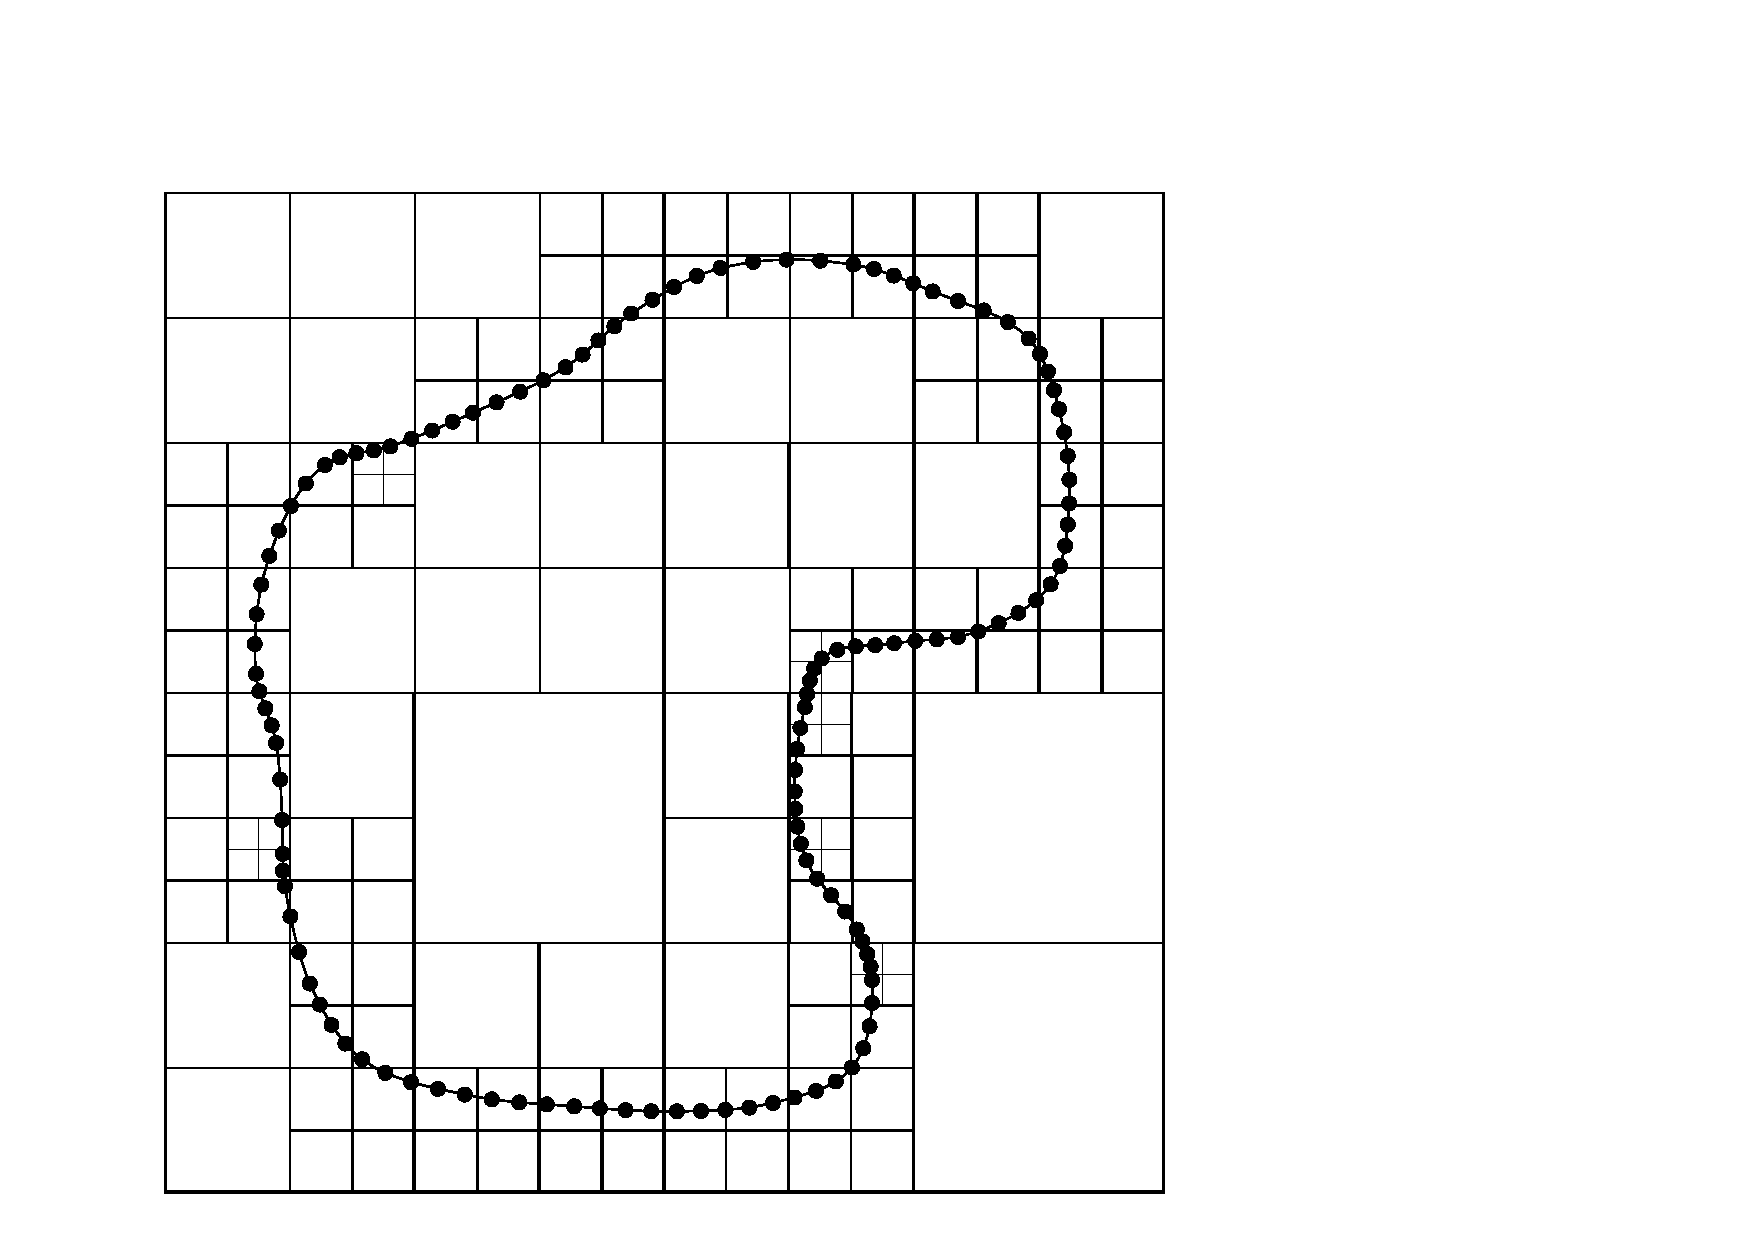
\includegraphics[width=12cm]{img/Quadtree.pdf}
	\caption{Adaptive quadtree in 2 dimensions}
	\label{fig:quadtree}
\end{figure}

The tree structure is then traversed, summing influences of near clusters directly (particle-particle) and evaluating the multipole approximations of distant clusters (cluster-particle). This delineation is controlled by a \emph{multipole acceptance criteria}, where a specified $\theta_{\text{MAC}}$ is compared to $\theta = b/d$, where $d$ is the distance between clusters and $b$ is a function of the size of the interacting clusters. If $\theta < \theta_{\text{MAC}}$ then the interaction is classed as short-range. This approach, represented by figure \ref{fig:treecode} gives a computational complexity of $\bigO(N\log N)$, enabling large calculations to be run in a reasonable timeframe.

\begin{figure}[h]
	\centering
	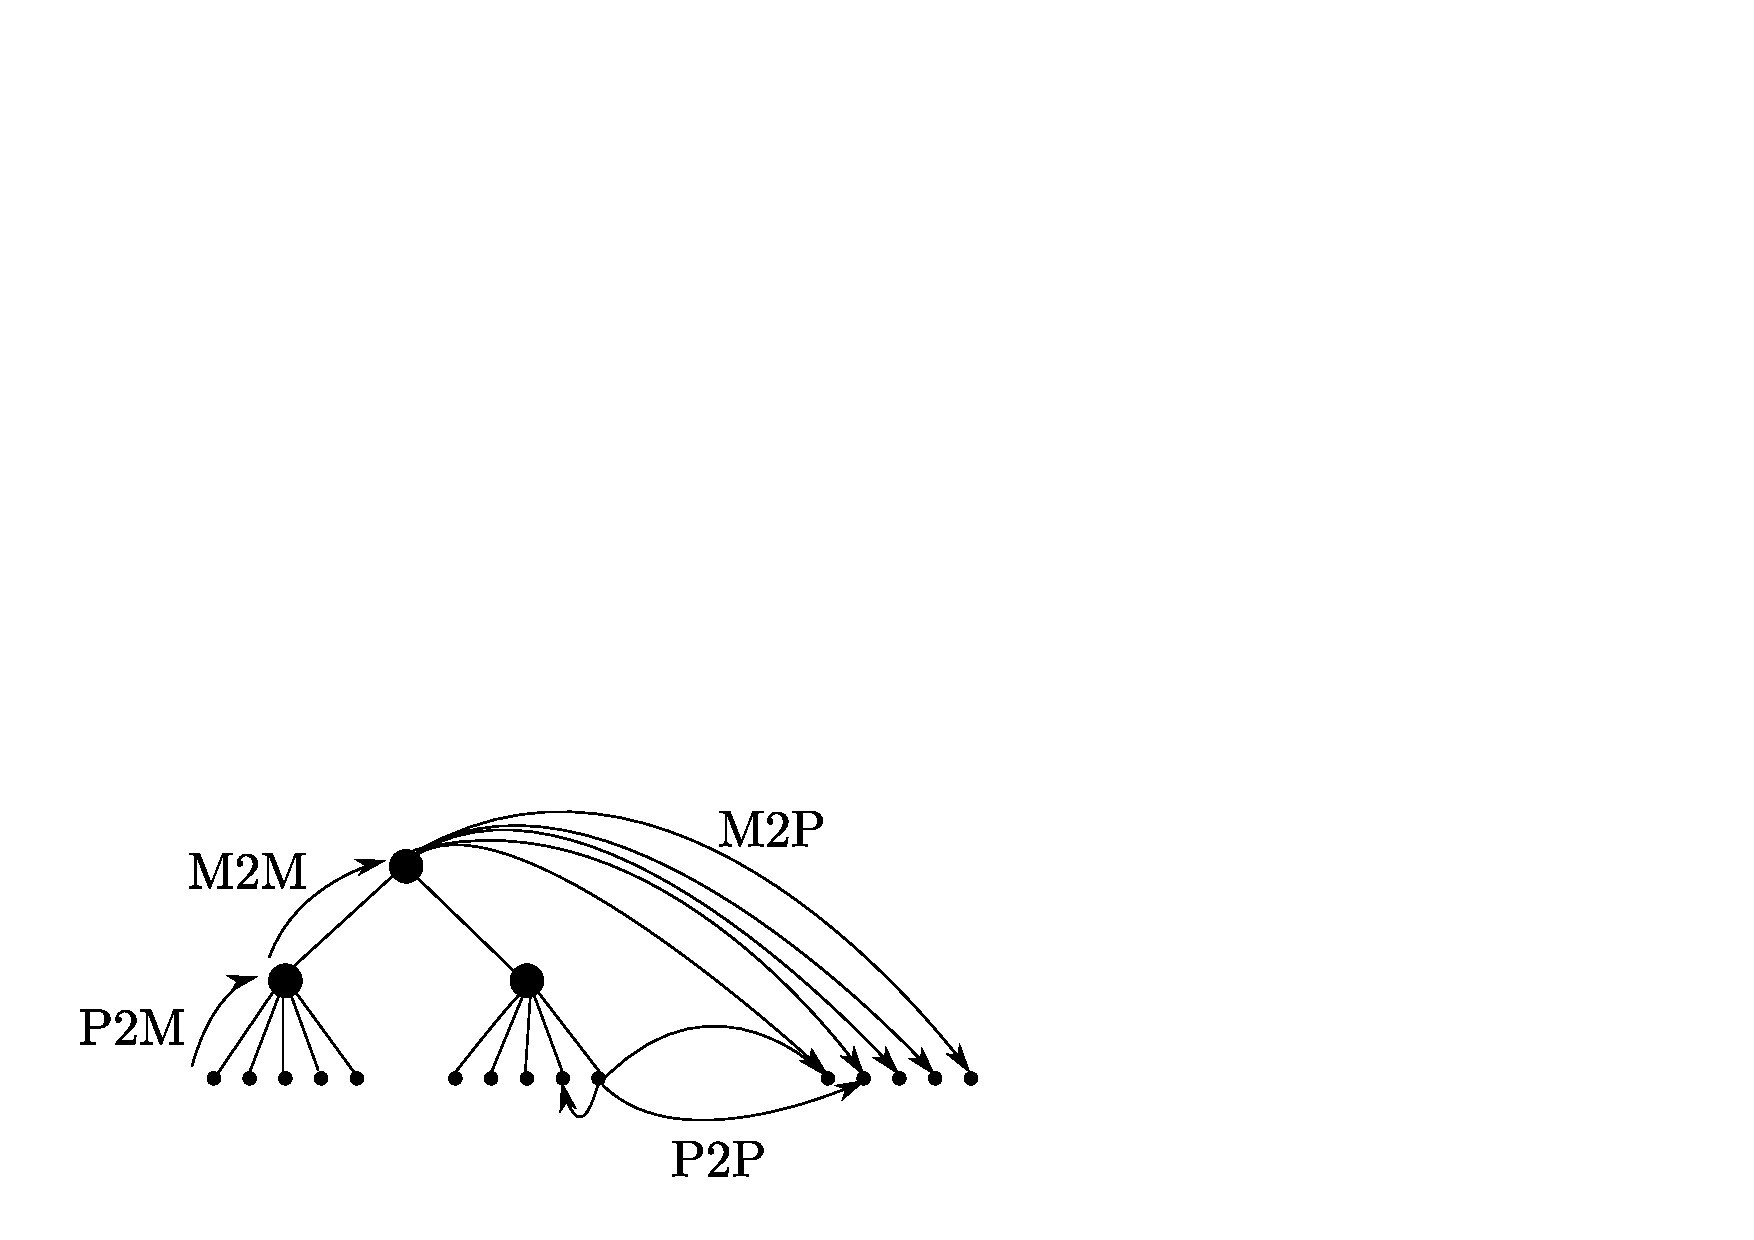
\includegraphics[width=10cm]{img/Treecode.pdf}
	\caption{Treecode}
	\label{fig:treecode}
\end{figure}

This method was later extended into the fast multipole method ({\fmm}) by Greengard \cite{greengard1987} to add local expansions which converge within a short distance of the expansion center. Instead of directly evaluating the multipole expansions of far clusters, the multipoles are translated and converted into local expansions (cluster-cluster), before being translated to the lowest nodes of the tree and evaluated against target points. Due to this modification, the overall complexity was reduced to the optimal $\bigO(N)$. A graphical representation of the algorithm is given in figure \ref{fig:fmm}. Later, support for other kernels, including Yukawa \cite{Boschitsch99,HuangJiaZhang2009} and Helmholtz \cite{GreengardETal1998} were added.

\begin{figure}[h]
	\centering
	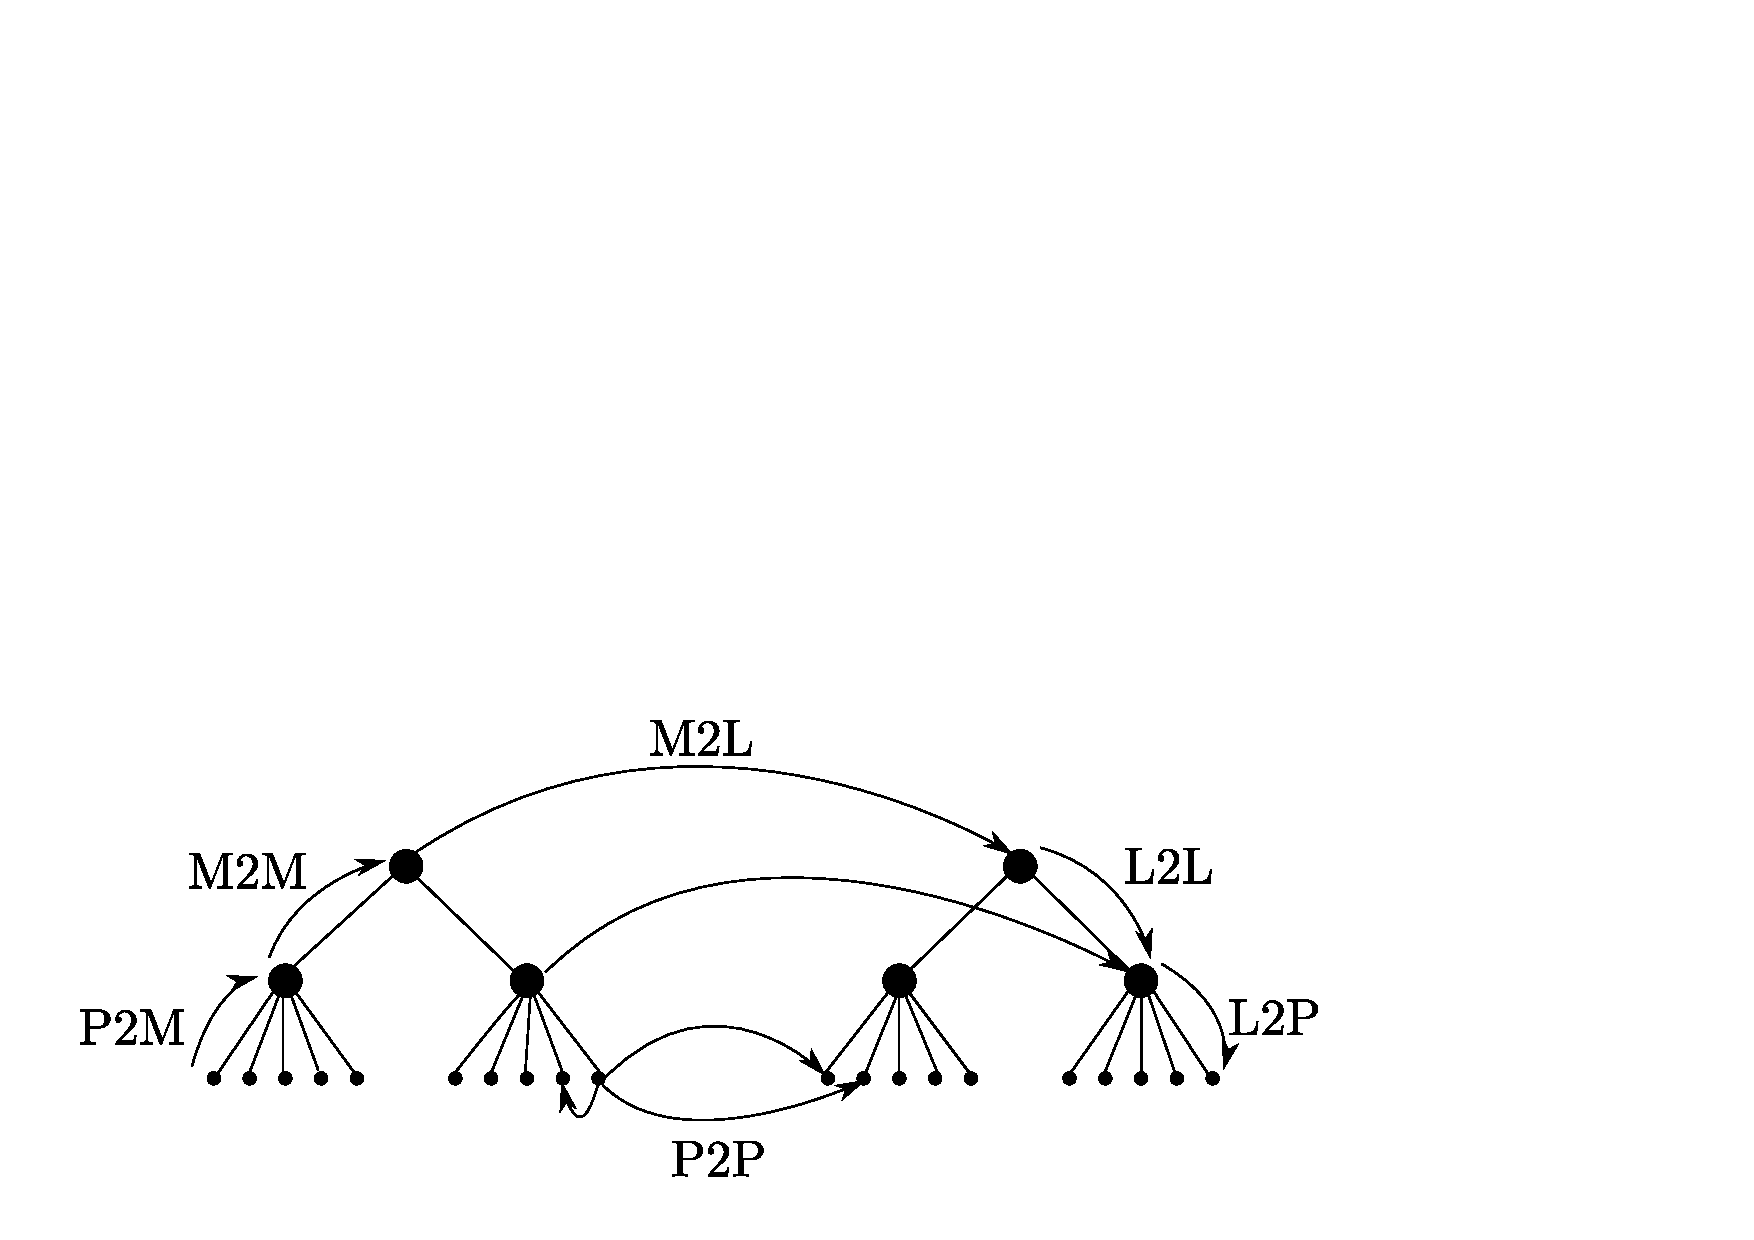
\includegraphics[width=12cm]{img/FMM.pdf}
	\caption{FMM}
	\label{fig:fmm}
\end{figure}

The {\fmm} can be used for any problem that has an n-body sum of the form of equation (\ref{eqn:nbody}) and a suitable Green's function. During each iterative solve step within the {\bem} we repeatedly compute sums of this kind due to evaluating integrals using Gauss quadrature --- repeated Green's function evaluations. Therefore, the {\fmm} can be used to accelerate this process.

{\fmm} and treecodes can be thought of as having 7 separate operators (or kernels) described in \S\ref{subsec:fmm_operators}, and 3 distinct ``phases'', summarised below in \S\ref{subsec:fmm_phases}. How these operators pertain to a tree structure is shown in figures \ref{fig:treecode} and \ref{fig:fmm} for treecodes and {\fmm}s respectively.

%%%%%%%%%%%%
% KERNELS
%%%%%%%%%%%%
\subsection{Operators}\label{subsec:fmm_operators}

There are 7 separate operators that constitute a standard {\fmm}, each performing a distinct operation, from directly evaluating the influence from one particle on another, to creating a multipole expansion, to translating series expansions up, down or across the tree. These operators are summarised below.

\begin{itemize}

\item \emph{Particle to Particle (P2P)} -- Calculate directly (using an $\bigO(N^{2}$) method) the interactions between source and target particles.

\item \emph{Particle to Multipole (P2M)} -- Generate a multipole expansion about a cluster center of all source particles contained within that cluster.

\item \emph{Multipole to Multipole (M2M)} -- Translate a multipole expansion by shifting it to a different center.

\item \emph{Multipole to Particle (M2P)} -- Evaluate a multipole expansion at a \emph{well-separated} target particle.

\item \emph{Multipole to Local (M2L)} -- Translate a multipole expansion to a \emph{well-separated} center point, and convert into a local expansion.

\item \emph{Local to Local (L2L)} -- Translate a local expansion to a different center.

\item \emph{Local to Particle (L2P)} -- Evaluate a local expansion at nearby particles.

\end{itemize}

\subsection{Phases of the FMM}\label{subsec:fmm_phases}

To perform a standard {\fmm}, we require 4 distinct phases, performed in order. Each of these phases is shown below, along with pseudocode for each phase.

\begin{itemize}

\item \emph{Tree Creation}, (algorithm \ref{alg:tree_construction}) -- The domain is partitioned hierarchically based on $N_{\text{CRIT}}$. Links between cells and their parents / children are created at this point for fast traversal later.

\begin{algorithm}
	\caption{Tree Construction}
	\label{alg:tree_construction}
	\begin{algorithmic}
		\Require Maximum \# of particles per cluster NCRIT, root cluster
		\State root = root\_cluster
		\For{sources, $j$}
			\State \Call{add\_to\_cluster}{$j$, root}
		\EndFor
		\State
		\Procedure{add\_to\_cluster}{point, cluster}
			\If{\Call{num\_points}{cluster} $<$ NCRIT}
				\State cluster.\Call{append}{point}
			\Else
				\If{not cluster.split}
					\State \Call{split}{cluster} \Comment Split into 8 child clusters
				\EndIf
				\State oct = \Call{octant}{point, cluster} \Comment Get correct child cluster
				\State \Call{add\_to\_cluster}{point, cluster.child[oct]}
			\EndIf
		\EndProcedure
	\end{algorithmic}
\end{algorithm}

\item \emph{Upward}, (algorithm \ref{alg:upward_sweep}) -- Multipole expansions are created at all leaf (lowest level) clusters (P2M). Then, expansions are translated up the tree to parent clusters (M2M). At the end of this stage, all clusters contain a multipole representation of all particles approximated by themselves and their descendants.

\begin{algorithm}
	\caption{Upward sweep}
	\label{alg:upward_sweep}
	\begin{algorithmic}
		\Require Cells $C$, kernel $K$.
		\For{i=1,\;...,\;\Call{size}{$C$}}
			\If{\Call{is\_leaf}{$C_{i}$}} 
				\State \Call{K.P2M}{points($C_{i}$)} \Comment Create multipole expansions at leaf cells
			\Else
				\State \Call{K.M2M}{$C_{i}$,\;parent($C_{i}$)}\Comment Translate multipole expansions up the tree
			\EndIf
		\EndFor
	\end{algorithmic}
\end{algorithm}

\item \emph{Interaction}, (algorithm \ref{alg:interaction}) -- Both long and short range interactions are calculated, based on interacting source and target clusters against each other. If the ratio $\theta = b / d$, where $d$ is the distance between 2 cluster centers, and $b$ is a function of the cluster sizes is less than some specified $\theta_{\text{MAC}}$, then direct particle-particle (P2P) evaluation is used. Otherwise, either cluster-particle (M2P) in the case of a treecode, or cluster-cluster (M2L) operators in the case of an {\fmm} are evaluated.

\begin{algorithm}
	\caption{Interaction Stage}
	\label{alg:interaction}
	\begin{algorithmic}
		\State pairQ = [\Call{root}{source}, \Call{root}{target}]
		
		\While{not \Call{empty}{pairQ}}
			\State pair = \Call{pop\_front}{pairQ}
			\State $b_{1}, b_{2}$ = pair.first, pair.second
			\If{\Call{is\_leaf}{$b_{1}$}}
				\If{\Call{is\_leaf}{$b_{2}$}} \Comment Both leaves -- direct evaluation
					\State \Call{P2P}{$b_{1}, b_{2}$}
				\Else
					\For{$bc$ in \Call{children}{$b_{2}$}}
						\State \Call{interact}{$b_{1}, bc$}
					\EndFor
				\EndIf
			\ElsIf{\Call{is\_leaf}{$b_{2}$}}
				\For{$bc$ in \Call{children}{$b_{1}$}}
					\State \Call{interact}{$bc,b_{2}$}
				\EndFor
			\Else
				\State \Call{interact}{...} \Comment Iterate over smaller box's children
			\EndIf
		\EndWhile
		\State
		\Procedure{interact}{$\text{Box}_{1}, \text{Box}_{2},$ pairQ} \Comment Interact two boxes
			\If{\Call{accept\_mac}{$\text{Box}_{1}, \text{Box}_{2}$}} \Comment Long-range interactions
				\If{FMM} 
					\State \Call{M2L}{$\text{Box}_{1}, \text{Box}_{2}$} \Comment Translate and convert multipole expansion
				\EndIf
				\If{TREECODE} 
					\State \Call{M2P}{$\text{Box}_{1}, \text{Box}_{2}$} \Comment Evaluate multipole at far points
				\EndIf
			\Else{}
				\State pairQ.\Call{push\_back}{pair($\text{Box}_{1}, \text{Box}_{2}$)} \Comment Not accepted, defer for splitting
			\EndIf
		\EndProcedure
	\end{algorithmic}
\end{algorithm}

\item \emph{Downward}, (algorithm \ref{alg:downward_sweep}) -- For a treecode, this phase is empty. For an {\fmm}, local expansions are propagated downwards through the tree (L2L), passing from a parent cluster to its children. At the leaf nodes, these local expansions are evaluated at all target points within each relevant cluster (L2P).

\begin{algorithm}
	\caption{Downward Sweep}
	\label{alg:downward_sweep}
	\begin{algorithmic}
		\For{all clusters, $c$}
			\If{not \Call{is\_leaf}{$c$}}
				\For{$ci$ in \Call{children}{$c$}}
					\State \Call{L2L}{$c, ci$} \Comment Translate local expansions down the tree
				\EndFor
			\Else{}
				\State \Call{L2P}{$c$} \Comment Evaluate local expansions at leaf cells
			\EndIf
		\EndFor
	\end{algorithmic}
\end{algorithm}
	
\end{itemize}

%%%%%%%%%%%%
% COMPLEXITY
%%%%%%%%%%%%
\subsection{Computational Complexity}

While we've already stated that the {\fmm} has $\O{N}$ scaling, we will now demonstrate it by breaking down the algorithm into distinct sections, giving the complexity of each section and thus the total complexity.

First of all, we define some useful values:

\begin{center}
\begin{tabular}{c|c}
	$N$ & Number of particles \\
	$l$ & Number of levels in the Octree, $\approx \log_8N$ \\
	$p$ & Truncation point of expansions \\
	$c_{\text{P2M}}(p)$ & Cost of a creating multipole expansion (single source) \\
	$c_{\text{M2M}}(p)$ & Cost of a single multipole-multipole translation \\
	$c_{\text{M2L}}(p)$ & Cost of a single multipole-local translation \\
	$c_{\text{L2L}}(p)$ & Cost of a single local-local translation \\
	$c_{\text{L2P}}(p)$ & Cost of evaluating a local expansion (single target) \\
	$N_{\text{M2L}}$ & Number of {\mtol} translations ($=189$)
	%$n$ & Cost of direct particle-particle between 2 boxes
\end{tabular}
\end{center}

Using these, we can form an estimate for the total runtime of the {\fmm} in terms of the cost of our expansions, which will then be specialized for a pair of different expansion types.
\begin{eqnarray}
	C_{\text{\fmm}} & = & N\cdot c_{\text{P2M}}(p) \nonumber \\
	& + & N\cdot c_{\text{M2M}}(p) \nonumber \\
 	& + & N\cdot N_{\text{M2L}}\cdot c_{\text{M2L}}(p) \label{eqn:fmm_costs} \\
	& + & N\cdot c_{\text{L2L}}(p) \nonumber \\
	& + & N\cdot c_{\text{L2P}}(p) \nonumber \\
	& + & N\cdot 27\cdot N_{\text{CRIT}}^{2} \nonumber
\end{eqnarray}

Clearly this shows that the total complexity is $\O{N}$ as long as $p \not= p(N)$, something that holds for all applications discussed in this thesis, and $\ncrit \ll N$, which holds for any reasonably created tree. (A notable application where $p = p(N)$ would be acoustics, using expansions for the Helmholtz Green's function). With a standard $\fmm$ formulation, $N_{\text{M2L}} = 189$. We can look at two examples, firstly Cartesian expansions, equation (\ref{eqn:cartesian_multipole})

\begin{equation}
	\phi(\vect{x}_i) = \sum_{||\vect{k}||=0}^{\vect{P}}\frac{1}{\vect{k}!}D^{k}_y(\vect{x_i},\vect{y})\psi(\vect{y}_j-\vect{y}_c)^{\vect{k}},
	\label{eqn:cartesian_multipole}
\end{equation}

where $\vect{k}$ is a multi-index variable, $\vect{k}=\{k_1, k_2, k_3\}$, $\vect{k}! = k_1!k_2!k_3!$, $\vect{y}^{k} = y_1^{k_1}y_2^{k_2}y_3^{k_3}$ and $D_y^{k} = D^{k_1}_{y_1}D^{k_2}_{y_2}D^{k_3}_{y_3}$ is the derivative operator. The other expansion we use as an example are spherical harmonic expansions, shown for Laplace's equation in equation (\ref{eqn:spherical_multipole}).

\begin{equation}
\phi(\vect{x}_i) = \sum_{n=0}^{p}\sum_{m=-n}^{n}\frac{Y^{m}_n(\theta_i,\phi_i)}{r_i^{n+1}}\left \{\sum_j^{N}q_j\rho^{n}_jY^{-m}_n(\alpha_i,\beta_i)\right \}
	\label{eqn:spherical_multipole}
\end{equation}

\begin{center}
	\begin{tabular}{c|c|c}
		Operation & Cost (Cartesian) & Cost (Spherical) \\ \hline
		$c_{\text{P2M}}$ & $\O{p^{3}}$ & $\O{p^{2}}$ \\
		$c_{\text{M2M}}$ & $\O{p^{6}}$ & $\O{p^{4}}$ \\
		$c_{\text{M2L}}$ & $\O{p^{6}}$ & $\O{p^{4}}$ \\
		$c_{\text{L2L}}$ & $\O{p^{6}}$ & $\O{p^{4}}$ \\
		$c_{\text{L2P}}$ & $\O{p^{3}}$ & $\O{p^{2}}$
	\end{tabular}
\end{center}

When we apply these costs to equation (\ref{eqn:fmm_costs}) we can immediately see that the most expensive expansion related cost will be the {\mtol} translations due to the large constant multiplier, given by $N\cdot N_{\text{M2L}}\cdot\O{p^{4}}$ for spherical expansions and $N\cdot N_{\text{M2L}}\cdot\O{p^{6}}$ for cartesian. The other most expensive part of the evaluation will be the direct near-field computation, given by $N\cdot 27\cdot \ncrit^{2}$. The fastest {\fmm} will usually involve trying to create a tree that keeps these two costs as equal as possible, known as \emph{well-balanced}. This balance comes from trying to ensure that $\ncrit$ does not become so large that the algorithm starts to scale as $\O{N^{2}}$, while making sure that the tree does not have so many levels that the number of {\mtol} translations becomes too large and dominates the run time. The high cost of {\mtol} translations is going to be one of the main motivators for the relaxation schemes introduced later in \S\ref{subsec:inexact_matvec}.

\section{Preconditioners}

In all the experiments performed in this work, an important metric is the number of iterations taken by our linear solver to converge to a solution. Given the cost of each iteration, this number will also heavily influence the total time-to-solution. The number of iterations will be most directly influenced by the \emph{condition number} of the matrix, $\kappa(A)$, given here for a normal matrix

\begin{equation}
	\kappa(A) = \left | \frac{\lambda_{\text{max}}(A)}{\lambda_{\text{min}}(A)} \right |,
\end{equation}

\noindent
where $\lambda_{\text{max}}$ and $\lambda_{\text{min}}$ are the largest and smallest eigenvalues of $A$ respectively. As the ratio of these eigenvalues gets closer to $1$, the matrix becomes more \emph{well-conditioned} and easier to solve (i.e. less solver iterations are needed).

In the context of Krylov solvers, one way to try and reduce the condition number is to apply a preconditioner, indicated in algorithm \ref{alg:gmres} by the step $Mz_j = v_j$ or

\begin{equation}
	z_{j} \gets M^{-1}\cdot v_{j},
\end{equation}

\noindent
with $M$ as some approximation to $A$. A simple example of $M$ is simply the diagonal of $A$, that is,

\begin{equation}
	M(A) = \text{diag}(A)
\end{equation}

%Note that the preconditioner, $M^{-1}$ can be thought of as a linear operator which operates on a vector. We can write this in a general form as $M^{-1}(x)$. This allows us to substitute any linear operator that will improve the solution as the operator $M^{-1}$. A simple example of this would be a diagonal preconditioner:
%
%\begin{equation}
%	M^{-1}(x) = \frac{x}{\text{diag}(A)}.
%\end{equation}

In this case, we can explicitly form $M^{-1}$, and applying the preconditioner is a simple element-wise multiplication between $M^{-1}$ and $v_j$ (\lstinline|axpy| in standard dense linear algebra notation). 

In general we may have to solve the $Mz_j = v_j$ system using a choice of linear solver (including another Krylov solver). The only additional overhead for this kind of so-call ``flexible'' preconditioner \cite{saad1993} from the viewpoint of the {\gmres} solver,  is a slightly increased memory footprint. There are multiple ways of modifying {\gmres} to accommodate this type of preconditioning; The one used in this thesis is {\fgmres}, algorithm \ref{alg:fgmres} \cite{saad1993}, simply {\gmres} as described in algorithm \ref{alg:gmres}, with two small changes: $V_{k} \gets [v_{1},...,v_{k}]$ changes to $Z_{k} \gets [z_{1},...,z_{k}]$ and we use $Z_{k}$ instead of $V_{k}$ when updating the approximation $x_{k}$. The {\fgmres} algorithm is shown in pseudocode as algorithm \ref{alg:fgmres}.

\begin{algorithm}
	\caption{Right-Preconditioned FGMRES \cite{saad1993}}
	\label{alg:fgmres}
	\begin{algorithmic}
		\Require Matrix $A$, initial guess $x_{0}$, right-hand side $b$, desired tolerance $\epsilon$, order of the Krylov space $k$, preconditioner $M$.
		\State Initialize $\bar{H}_{m} \in \R^{(k+1)\times k} = 0\;\forall i,j$
		\State $r_{0} \gets A\cdot x_{0}-b$
		\State $\beta \gets ||r_{0}||_{2},\;\; v_{1} \gets r_{0}/\beta$
		\For{j=1,...,k}
			\State $z_{j} \gets M^{-1}\cdot v_{j}$
			\State $w \gets A\cdot z_{j}$
			\For{i=1,..,j}
				\State $h_{i,j} \gets (w, v_{i})$
				\State $w \gets w - h_{i,j}\cdot v_{i}$
			\EndFor
			\State $h_{j+1,j} \gets ||w||_{2}$
			\State $v_{j+1} \gets w / h_{j+1,j}$
		\EndFor
		\State $Z_{k} \gets \left [z_{1}, ..., z_{k} \right]$
		\State $y_{k} = \arg\min_{y}||\beta e_{1} - \bar{H}_{k}y||_{2}$ and $e_{1} = [1,0,...,0]$
		\State $x_{k} \gets x_{0} + Z_{k}y_{k}$ 
	\end{algorithmic}
\end{algorithm}

Notice that the main cost per iteration is still the matvec $w \gets A\cdot z_{j}$, so the additional overhead of using the {\fgmres} variant is insignificant.

\section{Inexact Matrix-Vector Products}\label{subsec:inexact_matvec}

Consider the case where a matrix-vector product is not computed exactly, such as when using {\fmm} within {\gmres} or {\fgmres}. In this situation, $y \gets A\cdot x$ becomes $y \gets (A+\epsilon_{A})\cdot x$ with $\epsilon_A$ representing the errors induced by the {\fmm} approximation. It can be shown \cite{simonciniszyld2003} that not only will we still converge to the correct solution of the linear system, but that $||\epsilon_{A}||$ can grow as the residual becomes closer to the final desired tolerance. 

By introducing an error term on the $i$-th iteration to our matrix $A$, $E_i$, instead of the standard Arnoldi iteration used in {\gmres}, $AV_m = V_{m+1}H_{m}$, where $H_m$ is the upper-Hessenberg matrix produced from the Arnoldi iterations and $V_m = [v_1, v_2, \cdots, v_m]$, we use the \emph{inexact Arnoldi} iteration,

\begin{equation}
	[(A+E_1)v_1, \cdots, (A+E_m)v_m] = [v_1, \cdots, v_m]H_m.
\end{equation}

Assuming that the calculation of the initial residual, $r_0 = b-Ax_0$ is exact, and $\beta = ||r_0||$, we can write the $m$-th iteration of the {\gmres} procedure as $x_m = x_0 + \delta_mx$, with $\delta_mx = V_my_m$ and $y_m$ is the solution to $\min_y||H_my-\beta e_1||$. We diverge from the standard exact {\gmres} by introducing a perturbation matrix, $G_m = [E_1v_1, \cdots, E_mv_m]$. From here, we can write the inexact Arnoldi iteration as an exact Arnoldi iteration with

\begin{equation}
	(A+G_m V_m^{T})V_m = V_{m+1}H_m
\end{equation}

This shows that the quantities calculated in the first $i$ steps of an inexact Arnoldi iteration are exactly the same as the first $i$ steps of an exact iteration with $A = (A+G_mVM^{T})$. From this, we can use the standard {\gmres} results to show that the residual $r_m$ will decrease as $i$ grows, establishing the convergence of our inexact {\gmres}.

The convergence of an inexact {\gmres} solver has also been shown experimentally for dense linear algebra \cite{vandeneshofsleijpen2004,bourasfraysse2005,simonciniszyld2003}, and was implemented by explicitly adding a perturbation to $A$, such that $A' \gets A + A_\epsilon$ and $||A_\epsilon||$ is controlled as part of the relaxation strategy. A different approach \cite{sidjewinkles2011} has been used for sparse matrices, namely specifiying a ``drop-tolerance'', $\epsilon$, where if $||A_{ij}|| \leq \epsilon$, then that term is not counted when performing the matrix-vector products within {\gmres}.

We take a different approach with the {\fmm}, given that we can control error by using $p$ and $\theta_{\text{MAC}}$ as described in \S\ref{sec:fmm}. Given these values it is natural that we use them to adjust the accuracy of the {\fmm} for each iteration, reducing the accuracy to perform the minimum amount of work necessary, speeding up the calculation. We expect this to give a speedup due to the scaling of the {\fmm} --- the two main contributions to the {\fmm}'s runtime are, from \S\ref{sec:fmm}, the near-field calculation between boxes, taking $N\cdot27\cdot\ncrit^{2}$ time, and the {\mtol} translation stage, which takes $N\cdot N_{\text{M2L}}\cdot c_{\text{M2L}}(p)$ time. Given that $c_{\text{M2L}}(p) = \O{p^{4}}$ for a standard spherical harmonics expansion and $\O{p^{6}}$ for Cartesian series, the reduction in time can be significant as $p$ is reduced. For example, moving from $p = 10$ to $p=1$ is a potential $10^{4}\times$ reduction in work for the spherical harmonics case. While this level of acceleration is unlikely to be obtained in practise it shows the potential of reducing $p$ throughout the process of an iterative solve.

% The {\fmm} can control its error using the properties $p$ and $\theta_{\text{MAC}}$ described in \S\ref{sec:fmm}, so it is natural to take advantage, adjusting the accuracy of the {\fmm} for each iteration, in order to perform the minimum amount of work necessary, thus speeding up the calculation.

This method of controlling (and increasing) induced errors throughout the iterations of a linear solve is known as a \emph{relaxation scheme}. In chapter \ref{chapter:methods} we will describe the exact nature of a relaxation scheme, and look at the remaining numerical methods that will be used in order to perform experiments on a variety of sample {\bem} problems to demonstrate the application of relaxation schemes for {\fmmbem}. These experiments will constitute the first such work with relaxation schemes and {\fmmbem} solvers.

%We will now use these methods to perform experiments on a sample {\bem} problem, evaluating both the convergence of {\fmm}-{\bem}, and the effectiveness of our implemented preconditioners and relaxation strategies.

\cleardoublepage

% -------------------------------------
% CHAPTER 3: NUMERICAL METHODS
% -------------------------------------
%!TEX root = ../thesis.tex

\chapter{Numerical Methods}
\label{chapter:methods}
\thispagestyle{myheadings}

% set this to the location of the figures for this chapter. it may
% also want to be ../Figures/2_Body/ or something. make sure that
% it has a trailing directory separator (i.e., '/')!
\graphicspath{{Numerical_Methods/}}

%%%%% METHODS

This section describes in detail the exact numerical methods used in this thesis, along with relevant formulae and implementation details. We start by discussing the different types of numerical integrals that will be used, including analytical and semi-analytical routines for singular integrals. Finally, we provide details about the relaxation schemes that will form the basis of our experimentation, along with preconditioners that will be used along with and in competition to relaxation schemes.


%and which equations we will use for testing purposes. For each of the two example equations we experiment with, we derive the {\bem} formulation, as well as introduce the expansions used for the {\fmm}. Then, the treatment of integrals within {\bem} is discussed, including singular integrals with analytical and semi-analytical methods. Finally we provide details about the relaxation strategies and preconditioners we will use throughout our numerical experimentation.

%To experiment with all of the different components described in \S\ref{sec:background}, we have a brand-new {\fmm} code written from the ground up to be extensible, easy to use and simple to integrate into larger applications.
%
%The code is written in {\cpp}, extensively using {\cpp}11 features, using templates to provide  delineated components, such that any one component can be changed, and as long as it complies with a fixed interface, no other code need be changed. The major components are:
%
%\begin{enumerate}
%	\item \emph{Tree Structure} -- Decompose the domain into boxes, only needs to offer an interface to the boxes, the particles contained within leaf nodes, and the ability to query the connectivity between boxes (children and parents).
%	\item \emph{Evaluator} -- This is responsible for traversing the tree, and dictating exactly which operators are called, and in what order. For example, treecodes and {\fmm}s would merely have differing evaluators.
%	\item \emph{Kernel} -- This implements all of the needed operators for treecodes and/or FMMs. A minimal kernel need only have {\ptop}, {\ptom}, {\mtom} and {\mtop} operators (treecode). Further, we offer the ability to provide either serial or vectorized versions of operators -- for instance, a {\ptop} operation could be defined as point vs. point, or box vs. box. This allows  optimized kernels to be used if preferred, but lowers the initial cost of implementation.\end{enumerate}


%%%%%%%%%%%%%%%%%%%%%%%%%%%%
% STOKES
%%%%%%%%%%%%%%%%%%%%%%%%%%%%


%%%%% NUMERICAL INTEGRATION
\section{Numerical Integration}\label{subsec:numerical_integration}

For all the {\bem} formulations described in this work, we must integrate some function, $f(\vect{x},\vect{y})$ over a source panel, $\Gamma,\;\vect{y}\in\Gamma$ with respect to a target point, $\vect{x}$ in order to generate a matrix element. This section deals with how to perform these integrals with sources and targets in different parts of the domain.

\begin{equation}
	\int_\Gamma f(\vect{x},\vect{y})\;\di{\Gamma}.
\end{equation}

We can separate the types of integrals we need to perform in terms of the distance between the source panel and target point. We introduce the following terms to describe this separation:

\begin{itemize}

\item \emph{Far} -- Integrals where the source and target panels are far apart require much less accuracy than either of the 2 other categories. In order to accelerate the far-field evaluation for an {\fmm}, semi-analytical and analytical integrals are unsuitable, and in these cases, Gauss quadrature rules of low order ($\{1, 3, 4, 7\}$ quadrature points) are sufficient, fast, and suitable for acceleration using an {\fmm}.

\item \emph{Near-singular} -- This kind of integral occurs when the source panel and target point are close-by (defined somewhat arbitrarily), but not the same. The integral is non-singular, but still requires high accuracy.  High-precision versions of standard quadrature rules are suitable in these cases, or the analytical / semi-analytical methods developed for singular integrals can be re-used.

\item \emph{Singular} -- The integral of a singular function over a region that includes a singularity. In the case of {\bem}, this occurs when the target point is within the source panel. Due to the singularity, most standard approximation techniques cannot be used, and so special methods must be developed, such as analytical or semi-analytical integrals.
	
\end{itemize}

The domain for each of these methods is shown graphically in figure \ref{fig:integration_domain}, and methods for each along with an implemented example are described in the following sections.

\begin{figure}[h]
	\begin{centering}
	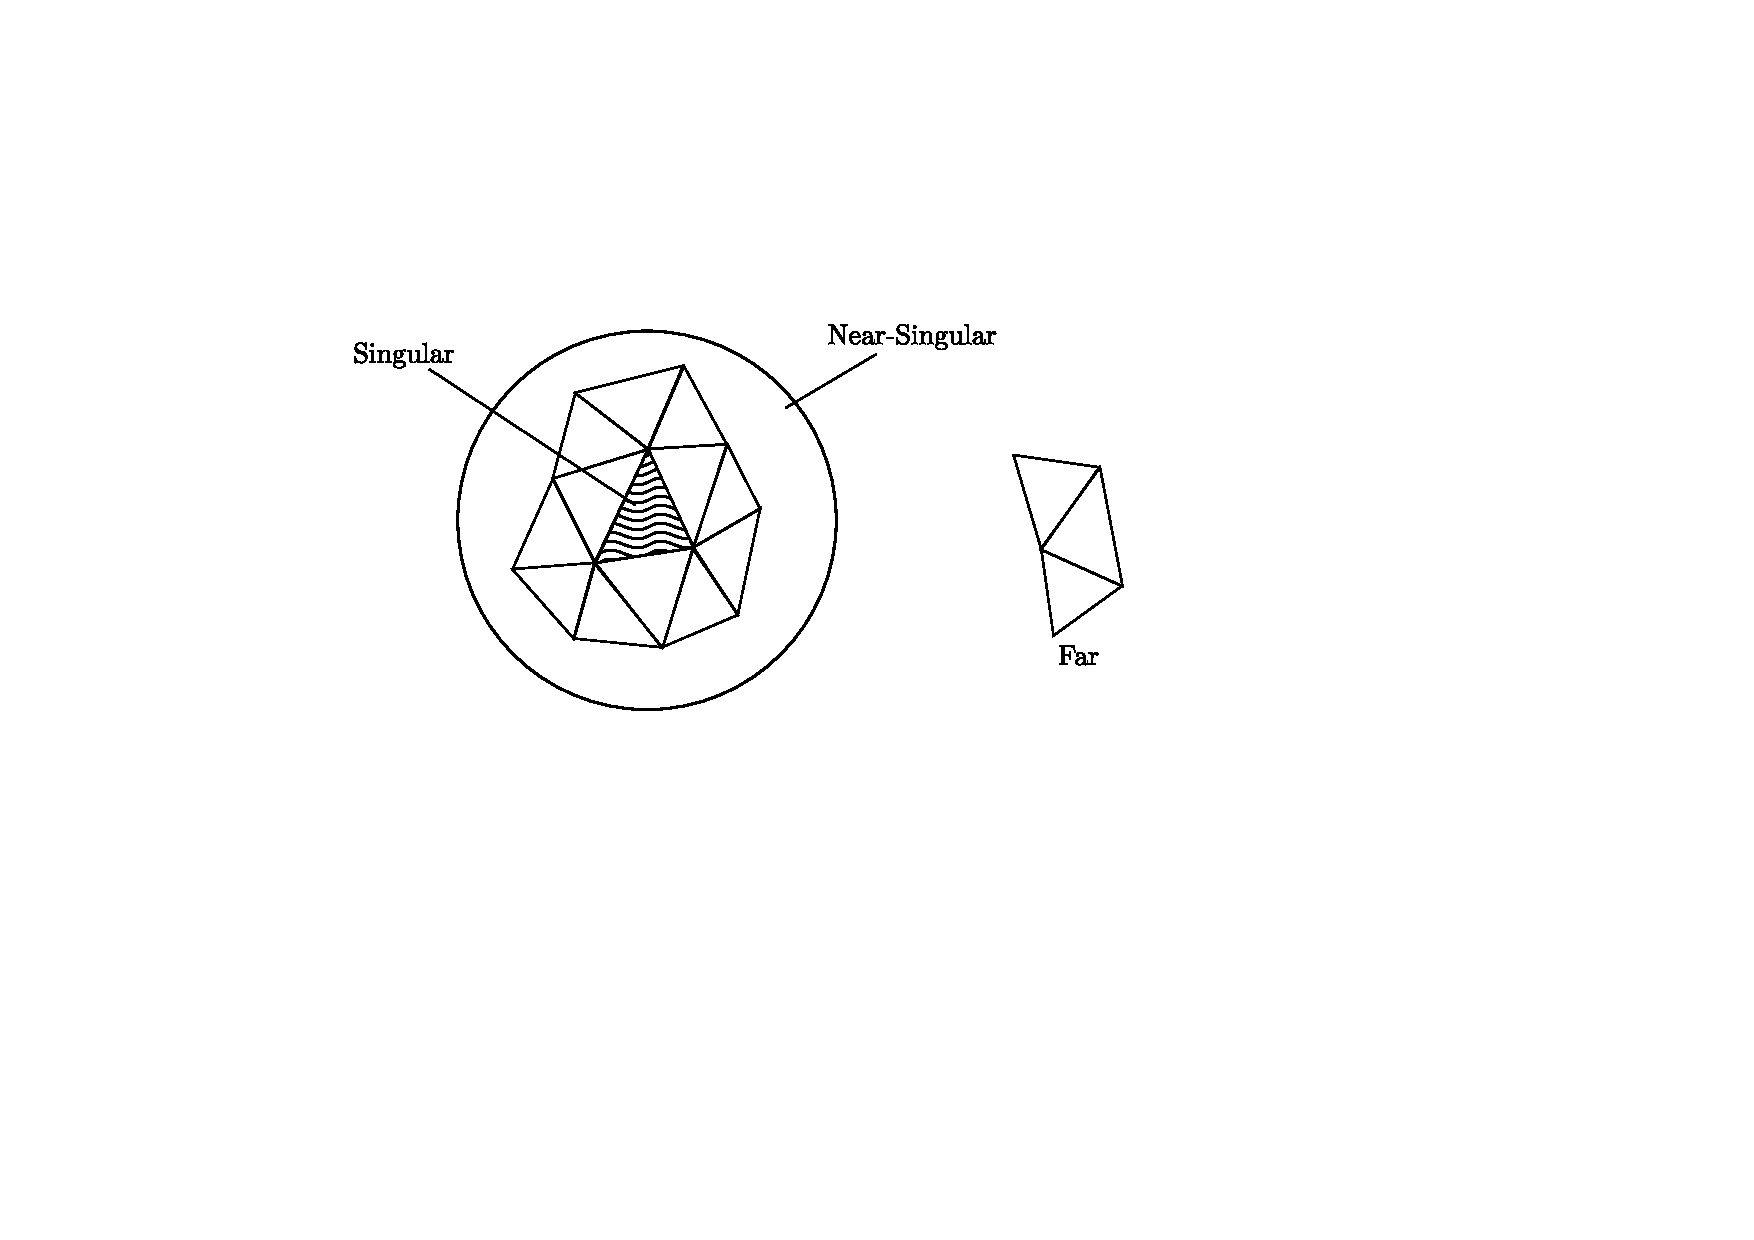
\includegraphics[width=12cm]{img/IntegrationDomain.pdf}
	\caption{Integration domains}
	\label{fig:integration_domain}
	\end{centering}
\end{figure}

%%%%%%%%%%%%%%%%%%%%%%%%%%%
% GAUSS QUADRATURE
%%%%%%%%%%%%%%%%%%%%%%%%%%%
\subsection{Gauss Quadrature}\label{subsubsec:quadrature}

Gaussian quadrature is an approximation to a definite integral, formed by a weighted sum of $K$ function evaluations at $K$ \emph{gauss points}, $x_k$ and \emph{gauss weights}, $w_k$ within the integration region. As a 1D example, consider the integral of a single-valued function, $f(x)$ over a line segment, $[a,b]$.

\begin{equation}
	\int_a^{b} f(x)\;\di{x} \approx \sum_{k=1}^{K} w_k f(x_k), \;\; w_k\in[0,1],\; x_k \in [a,b].
	\label{eqn:quadrature_1}
\end{equation}

This method is generalizable over $n$-dimensions, so for a multi-variate function $f(\vect{x}),\;\vect{x}\in\R^{d}$ defined in some region, $\D$, \ref{eqn:quadrature_1} changes very little, to

\begin{equation}
	\int_{\D} f(\vect{x})\;\di{\vect{x}} \approx \sum_{k=1}^{K} w_k f(\vect{x}_k), \;\; w_k\in[0,1],\; \vect{x}_k \in \D.
	\label{eqn:quadrature_2}
\end{equation}

For an example of this, we can look at the integrals resulting from the {\bem} formulation for the Laplace equation, given later in equations \ref{eqn:laplace_bem_G} and \ref{eqn:laplace_bem_dGdn}. In this case, $\vect{x}_i$ is a target point, and $j$ denotes a particular panel. Using a rule of the form from \ref{eqn:quadrature_2} these integrals turn into

\begin{eqnarray}
	\int_{\Gamma} G(\vect{x}_i,\vect{x}_j)\;\di{\Gamma_j} & \approx & \sum_{k=1}^{K} w_k\cdot A_j\cdot \frac{1}{|\vect{x}_i-\vect{x}_k|},\;\;\vect{x}_k \in \Gamma_j, \\ 
	\int_{\Gamma} \partiald{G(\vect{x}_i,\vect{x}_j)}{\nhat_j}\;\di{\Gamma_j} & \approx & \sum_{k=1}^{K}w_k\cdot A_j\cdot \frac{d\vect{x}\cdot\nhat_j}{|\vect{x}_i-\vect{x}_k|^{3}},\;\;\vect{x}_k \in \Gamma_j,
\end{eqnarray}

\noindent
where $w_k$ are area-normalized Gauss quadrature weights and $A_j$ is the area of $\Gamma_j$. The accuracy of the integral can be controlled by changing the number of quadrature points used, $K$. Common values for far integrals include $K=3,4$, while near-singular, many more Gauss points, for instance $K=19, 25$ may be necessary. It is worth noting here that both integrals are now expressed in terms of repeated evaluations of $1/r$ and $\nabla (1 / r)\cdot\nhat_j$, making them suitable for use with an {\fmm} and enabling us to speedup the solution to the linear system. %  It is this property that we use to enable the speedup of the solution to our system using {\fmm} and treecodes.

Each quadrature point is expressed in terms of a set of normalized co-efficients and an area-normalized weight. Given a set of co-efficients $\xi_1,\;\xi_2,\;\xi_3$, we can express the associated quadrature point, $(x_p,y_p,z_p)^{T}$ on a triangle defined by 3 vertices, $(x_1,y_1,z_1),\;(x_2,y_2,z_2),\;(x_3,y_3,z_3)$ in the following way:

\begin{equation}
\left (
	\begin{array}{c}
	x_p \\
	y_p \\
	z_p
	\end{array}
	\right ) = \left ( \begin{array}{ccc}
				x_1 & x_2 & x_3 \\
				y_1 & y_2 & y_3 \\
				z_1 & z_2 & z_3
				\end{array} \right )	\times \left ( \begin{array}{c}
													\xi_1 \\
													\xi_2 \\
													\xi_3
												   \end{array}\right ).
\end{equation}

This allows us to use the same sets of quadrature co-efficients for every integral without any changes. We use both standard low-order quadrature rules, with $k=3,4,7$, but also have much higher-precision options available for near-singular integrals. Our default rule for near-singular integrals uses $k=25$, while even higher precisions are available, for instance $k=79$.

Example co-efficients for $K=3$ for a triangular panel are given in table \ref{tab:gauss_weights_k3}.

\begin{table}[h]
\begin{center}
\begin{tabular}{c|cccc}
 $k$ & $\xi_1^{k}$ & $\xi_2^{k}$ & $\xi_3^{k}$ & $w_k$ \\
  & & & & \\
 1 & 1/2 & 1/2 & 0 & 1/3 \\
  & & & & \\
 2 & 0 & 1/2 & 1/2 & 1/3 \\
  & & & & \\
 3 & 1/2 & 0 & 1/2 & 1/3
 
\end{tabular}
\end{center}
\caption{Co-efficients and weights for Gauss integration over a triangular panel, $K=3$}
\label{tab:gauss_weights_k3}
\end{table}%

%[[[ ADD EXAMPLES OF CO-EFFICIENTS AND WEIGHTS? ]]]

%%%%%%%%%%%%%%%%%%%%%%%%%%%
% SEMI ANALYTICAL INTEGRALS
%%%%%%%%%%%%%%%%%%%%%%%%%%%
\subsection{Semi-Analytical}\label{subsubsec:semi_analytical}

The first approach for singular and near-singular integrals, will deal with the case that the function being integrated is (excluding constants) only a function of $r$, that is, $f = f(r)$, and $\int_a^{b} f(r)\;\di{r}$ can be computed analytically.

The technique we will describe relies on the fact that the integral over a polygon can be decomposed into a \emph{signed summation} of the triangles resulting from the projection of the target point onto the polygon plane, denoted $P$, and two of the polygon vertices. In this way

\begin{equation}
	\int_\Gamma f(r)\;\di{r} = \sum_{i=0}^{\# \text{vertices}} s_i \int_{PV_iV_{i+1}} f(r)\;\di{r},
\end{equation}

\noindent
where $s_i$ is the signing term, given by $1$ if $v_iv_{i+1}$ is clockwise from the target point, and $-1$ otherwise. This composition is shown in figure \ref{fig:semi_analytical_decomposition}.


\begin{figure}[ht]
\begin{center}
	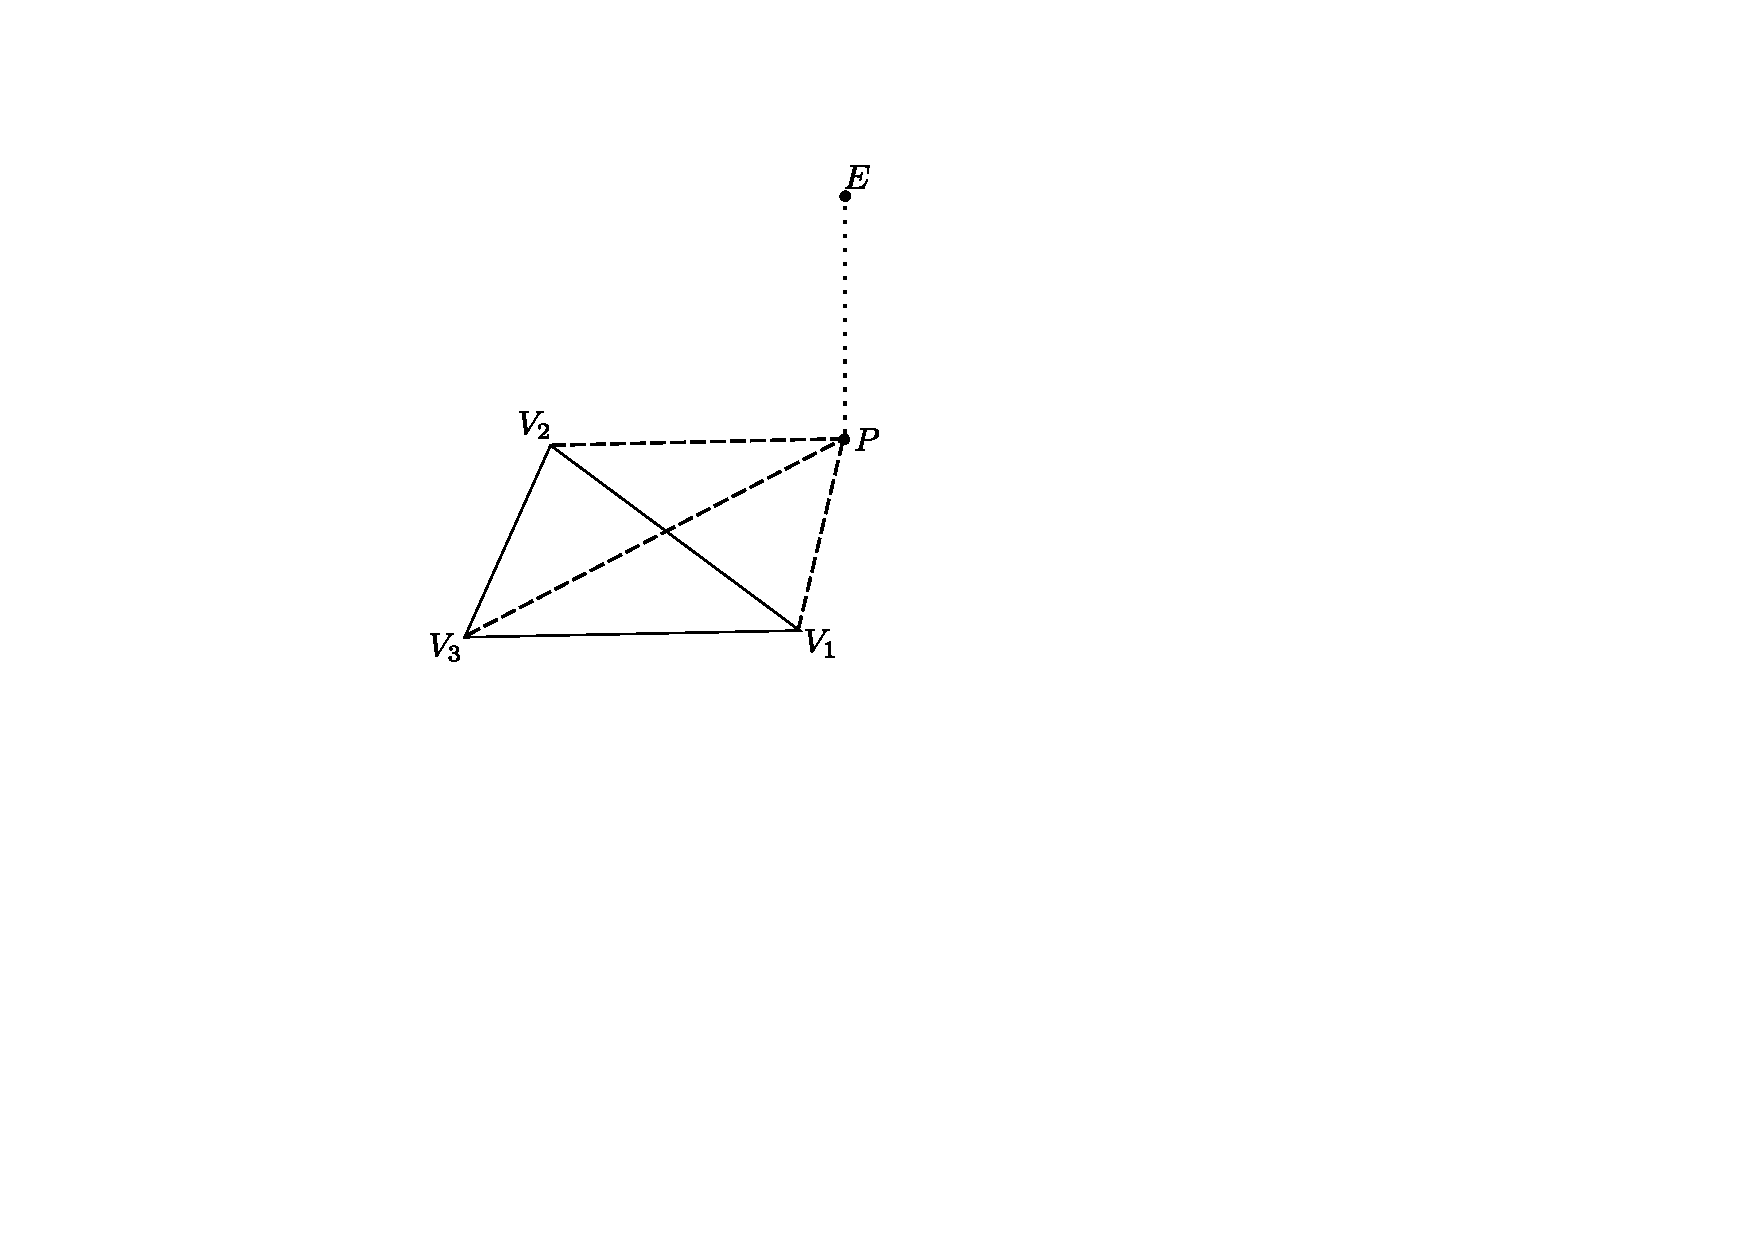
\includegraphics[width=8cm]{img/SemiAnalyticalDecomposition.pdf}
	\caption{Integral decomposition into triangles}
	\label{fig:semi_analytical_decomposition}
	\end{center}
\end{figure}


\begin{figure}[ht]
\begin{center}
	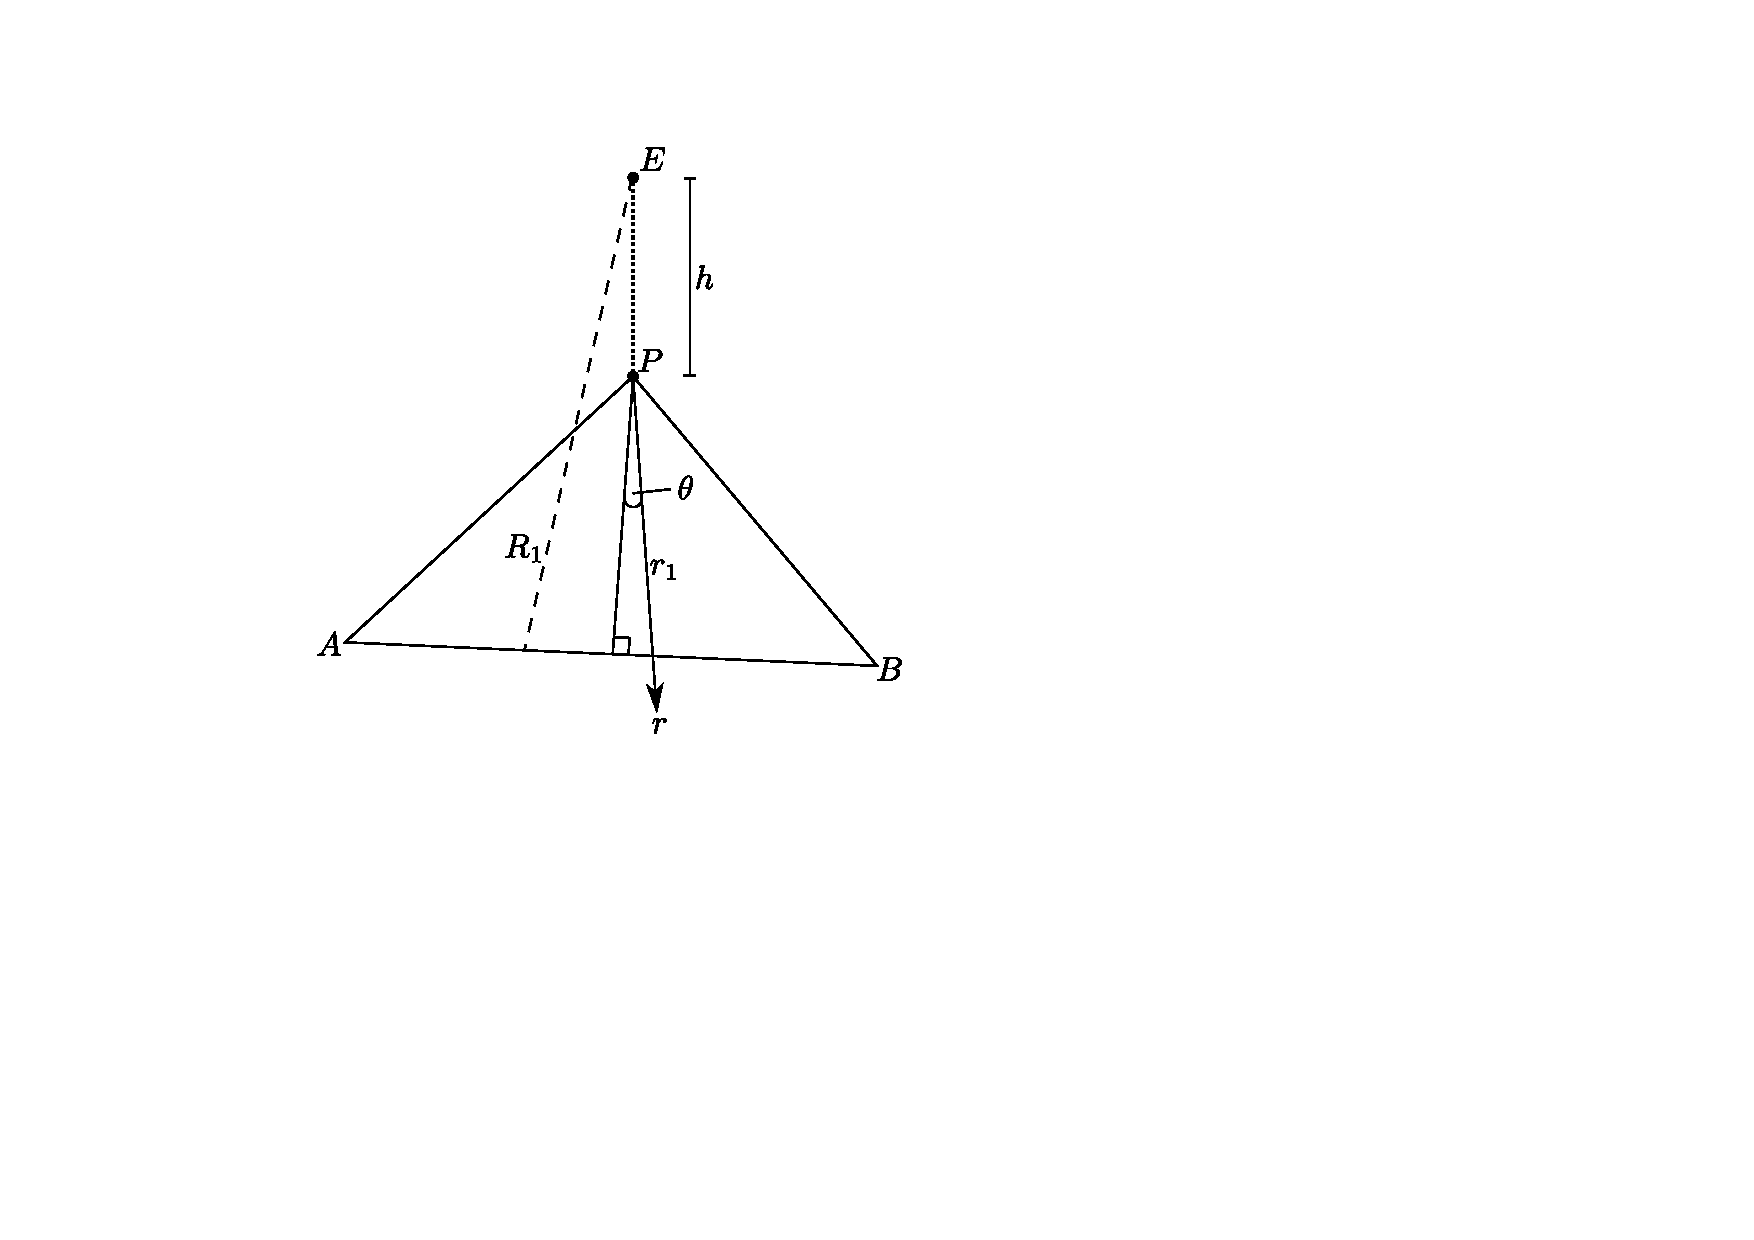
\includegraphics[width=8cm]{img/SemiAnalyticalIntegral.pdf}
	\caption{Individual triangular integral setup}
	\label{fig:semi_analytical_integral}
\end{center}
\end{figure}

For each of the individual integrals, we set up the integration domain, figure \ref{fig:semi_analytical_integral}, noting that $R = \sqrt{r^{2}+h^{2}}$ and then
\begin{eqnarray}
	\frac{\text{d}R}{\text{d}r} & = & \frac{r}{\sqrt{r^{2}+h^{2}}} \nonumber \\
	\text{d}R & = & \frac{r}{R}\;\text{d}r \nonumber \\
	R\;\text{d}R & = & r\;\text{d}r \nonumber
\end{eqnarray}

If we denote the integral over this triangle by $I$, then we can now write

\begin{eqnarray}
	I & = & \int_{\theta_1}^{\theta_2}\int_0^{r_1(\theta)} f(r)\cdot r\;\di{r}\;\di{\theta} \nonumber \\
	    \label{eqn:inner_1} & = & \int_{\theta_1}^{\theta_2}\int_h^{R_1(\theta)} f(R)\cdot R\;\di{R}\;\di{\theta}.
\end{eqnarray}

Similarly, to find the integral of the derivative of $f(r)$ in a direction, $\partialdi{I}{x_i}$, we can perform

\begin{equation}
	\label{eqn:inner_2}
	\partiald{I}{x_i} = \partiald{}{x_i} \int_{\theta_1}^{\theta_2} \int_h^{R_1(\theta)}f(R)\cdot R \;\di{R}\;\di{\theta}
\end{equation}

The inner integrals in equations \ref{eqn:inner_1} and \ref{eqn:inner_2} over $R$ will be performed analytically, then the outer integral over $\theta$ will be done using gaussian quadrature. As a first example, we look at the Green's function for Laplace's equation, $f(R) = 1 / R$
\begin{eqnarray}
	\int_h^{R_1(\theta)} f(R)\cdot R\;\di{R} & = & \int_h^{R_1(\theta)}1\;\di{R} \nonumber \\
	& = & R_1(\theta) - h. \nonumber \\
	\partiald{}{\nhat}\int_h^{R_1(\theta)} f(R)\cdot R\;\di{R} & = & \partiald{R_1(\theta)}{\nhat} -\partiald{h}{\nhat} \nonumber \\ 
	& = & \frac{z}{R(\theta)}-\text{sign}(z) \nonumber
\end{eqnarray}

Next, we look at the Yukawa equation, $f(R) = \exp(-kR) / R$

\begin{eqnarray}
	\int_h^{R_1(\theta)} f(R)\cdot R\;\di{R} & = & \int_h^{R_1(\theta)}e^{-kR}\;\di{R} \nonumber \\
	& = & -\frac{1}{k}\left [ e^{-kR_1(\theta)} - e^{-kh}\right ] \nonumber \\
	\partiald{}{\nhat}\int_h^{R_1(\theta)} f(R)\cdot R\;\di{R} & = & \frac{z\cdot e^{-kR(\theta)}}{R(\theta)} - e^{-kR(\theta)}\cdot\text{sign}(z) \nonumber
\end{eqnarray}

Now that we have the singular integrals available for Laplace and modified-Helmholtz, it is time to tackle the integrals that this semi-analytical method is unsuitable for -- the Green's functions for the Stokes equation. This will be handled with an analytical expression.

%%%%%%%%%%%%%%%%%%%%%%%%%%%
% ANALYTICAL
%%%%%%%%%%%%%%%%%%%%%%%%%%%
\subsection{Analytical}\label{subsubsec:analytical}

For functions that cannot be expressed purely in terms of $f(r)$, we need a different approach to the semi-analytical one described in \ref{subsubsec:semi_analytical}. In these cases, we have chosen to use a purely analytical method, described by S. Fata for both Laplace \cite{fata2009} and linear elasticity \cite{fata2011}, and trivially adaptable for the Stokes equations.

We begin with a triangle described by its 3 vertices, $\vect{y}_1, \vect{y}_2$ and $\vect{y}_3$, defined in a clockwise direction. In this way, the 3 line components of the triangle are described in terms of the vertices, with $L_1 = [\vect{y}_1, \vect{y}_2]$, $L_2 = [\vect{y}_2, \vect{y}_3]$, $L_3 = [\vect{y}_3, \vect{y}_1]$. The plane in which the triangle lies is denoted by $E_q$. Next, we compute an orthonormal companion reference $\{\vect{e}_1, \vect{e}_2, \vect{e}_3 \}$, designed so that $\vect{e}_1$ is parallel to $L_1$, and $\vect{e}_3$ is perpendicular to the edges of the triangle and points in the direction of the outward normal. The plane spanned by $\vect{e}_1$ and $\vect{e}_2$ is referred to by $P_{E_q}$. Thus, we introduce a new co-ordinate system, $\vect{x}; \xi, \zeta, \eta$ that is associated with $E_q$, shown in figure \ref{fig:fata_local_coordinate}.

\begin{figure}[hc]
\begin{centering}
	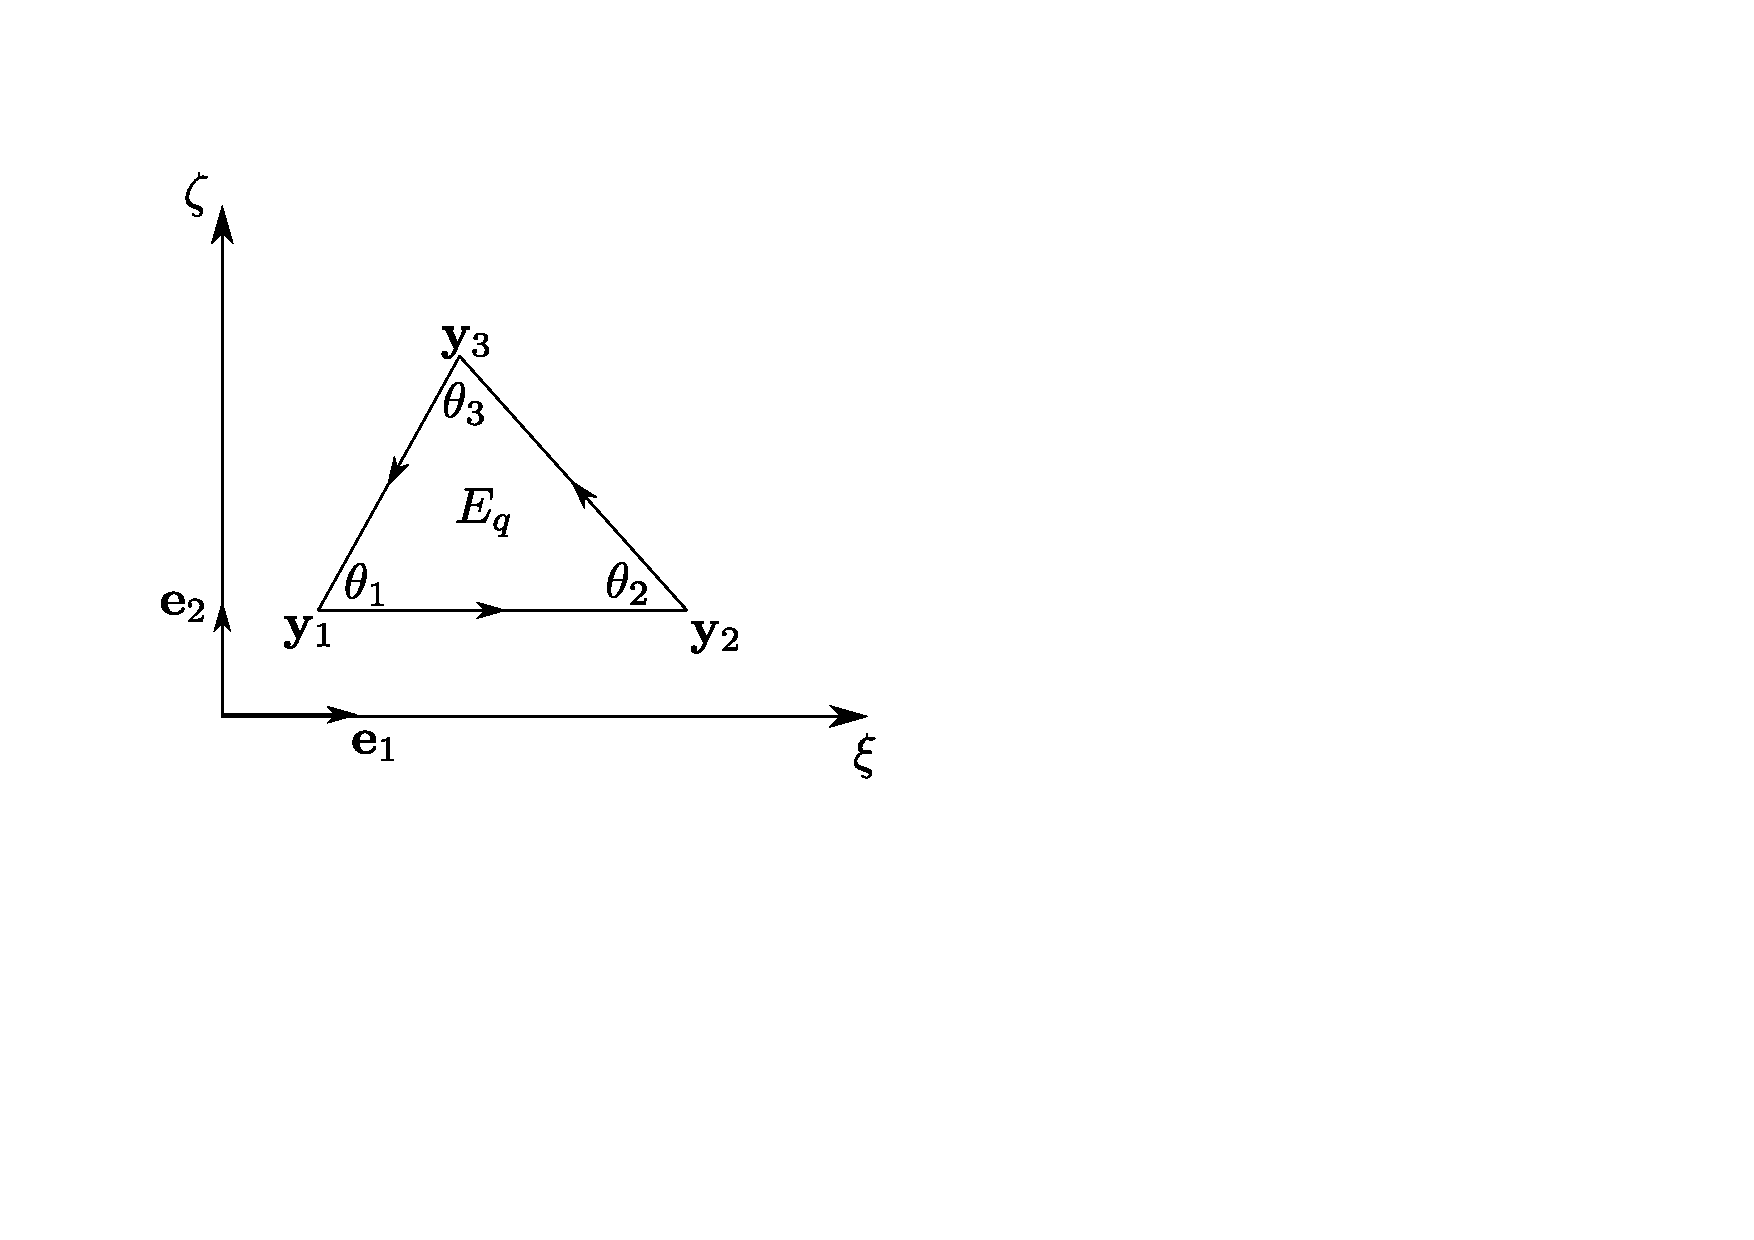
\includegraphics[width=10cm]{img/FataGeometry.pdf}
	\caption{Local co-ordinate system for analytical integrals}
	\label{fig:fata_local_coordinate}
\end{centering}
\end{figure}

Using this co-ordinate system, we can describe important quantities which are used to describe our integrals in the forms shown in equations \ref{eqn:generic_int1} and \ref{eqn:generic_int2}.
\begin{eqnarray*}
	\vect{r} & = & \vect{y}-\vect{x} = \xi\vect{e}_1 + \zeta\vect{e}_2 + \eta\vect{e}_3 \\ 
	r & = & ||\vect{y}-\vect{x}|| = \sqrt{\xi^{2} + \zeta^{2} + \eta^{2}},
\end{eqnarray*}
%
%\noindent
%that we can use to describe our integrals in the following forms:

\begin{eqnarray}
	\int_{\Gamma_j} G(\vect{x},\vect{y}) \di{\Gamma_j} & = & \frac{1}{4\pi}I_1 \label{eqn:generic_int1}\\
	& & \nonumber \\
	\int_{\Gamma_j} \partiald{G_j(\vect{x})}{\nhat} \di{\Gamma_j} & = & -\frac{\eta}{4\pi}I_3, \label{eqn:generic_int2}
\end{eqnarray}

\noindent
where the generic integrals $I_1,\; I_3$ refer to:

\begin{equation}
	I_1 = \int_{E_q} \frac{1}{r} \di{s}, \;\;\;I_3 = \int_{E_q} \frac{1}{r^{3}} \di{s}
\end{equation}

To express these generic integrals, we must define some more quantities over the panel. First, $\theta_i \in (0,\pi)$ is the inclusion angle at vertex $i$, such that $\theta_1 + \theta_2 + \theta_3 = \pi$, next we define $\alpha_1 = 0,\;\alpha_2 = \pi-\theta_2,\;\alpha_3 = \pi + \theta_1$. Using these values of $\theta_i$ and $\alpha_i$ we can constuct a set of 3 local orthonormal bases centred at the origin, given by $\{\vect{e}_{p_i}, \vect{e}_{q_i}, \vect{e}_3\}$, such that $\vect{e}_{p_i}$ is parallel to the previously defined line $L_i$. This gives us local coordinated systems, denoted by $\{p_i, q_i, \eta\}$ that are associated with each edge of the triangle. In this form, we have
\begin{equation}
	p_i = \xi\cos\alpha_i + \zeta\sin\alpha_i, \;\;\;\;q_i = -\xi\sin\alpha_i + \zeta\cos\alpha_i.
\end{equation}

More local coordinate systems can be formed from this construction, $\utilde{\vect{x}} = (p_i, q_i)$ defined for each of the sides of the triangle, allowing us to write a local coordinate $(p_i^{j},q_i^{j},\eta)$ in terms of a basis $\{\vect{e}_{p_i}, \vect{e}_{q_i}, \vect{e}_3\}$. The distance $\rho_j$ between a vertex, $\vect{y}_i$ and a source point, $\vect{x}$ can now be written as
\begin{equation}
	\rho_j = \sqrt{(p_i^{j})^{2} + (q_i^{j})^{2}+\eta^{2}}.
\end{equation}

To make the following equations simpler, we define
\begin{equation}
	\tilde{\rho}_1 = \rho_1-\rho_2,\;\;\tilde{\rho}_2 = \rho_2 - \rho_3,\;\;\tilde{\rho_3} = \rho_3-\rho_1,\;\;d_i = (q_i)^{2} + \eta^{2},\;\;i = 1,2,3.
\end{equation}

More quantities are now defined over each side, $L_i$,

\begin{equation}
	\gamma_i(\vect{x}) = \arctan\left ( \frac{-2p^{i}_iq_i\eta\rho_i}{(q_i)^{2}(\rho_i)^{2}-(p_i^{i})^{2}\eta^{2}} \right ) - \arctan\left ( \frac{-2p_i^{i+1}q_i\eta\rho_{i+1}}{(q_i)^{2}(\rho_{i+1})^{2}-(p_i^{i+1})^{2}\eta^{2}} \right )
\end{equation}
\begin{eqnarray}
	\chi_i(\vect{x}) & = & \ln(p_i^{i}+\rho_i) - \ln(p_i^{i+1}+\rho_{i+1}), \\ 
	\delta_i(\vect{x}) & = & \frac{p_i^{i}}{\rho_i} - \frac{p_i^{i+1}}{\rho_{i+1}}, \\
	\L_i(\vect{x}) & = & \frac{1}{\rho_i} - \frac{1}{\rho_{i+1}}.
\end{eqnarray}

Discarding all explicit dependancies on $\vect{x}$ for brevity's sake, we define the last couple of quantities needed, $\theta_0(\vect{x})$, dependant on the location of the center of the source panel and $\theta(\vect{x})$.

\begin{equation}
	\theta_0(\vect{x}) = 
	\begin{cases}
		0 & \text{if}\; \utilde{\vect{x}} \in P_{E_q}\setminus \bar{E_q} \\
		\pi & \text{if}\; \utilde{\vect{x}} \in \L_q\setminus\{ \vect{y}_1, \vect{y}_2, \vect{y}_3 \} \\
		2\pi & \text{if}\; \utilde{\vect{x}} \in E_q \\
		\theta_i & \text{if}\; \utilde{\vect{x}} = \vect{y}_i, \;\; i=1,2,3
	\end{cases}
\end{equation}

\begin{equation}
	\theta(\vect{x}) = \frac{1}{2}\sum_{i=1}^{3}\gamma_i(\vect{x}) + \sign(\eta)\theta_0(\vect{x})	
\end{equation}

This allows us to finally define $I_1$ and $I_3$ as:

\begin{eqnarray}
	I_1 & = & \sum_{i=1}^{3} q_i\chi_i(\vect{x}) - \eta\theta(\vect{x}) \\ 
	I_3 & = & \frac{1}{\eta} \theta(\vect{x}),
\end{eqnarray}

\noindent
allowing us to compute the desired integrals.

This work on analytical integrals for potential problems was later extended to linear elasticity integrals \cite{fata2011}, which can then be devolved into Stokes kernels by setting the poisson ratio, $\nu = 1 / 2$. By using the same quantities over the triangle as from the potential integrals, we can express these Stokes integrals in a similar fashion

\begin{eqnarray}
	U(\vect{x},\vect{y}) & = & \frac{1}{8\pi\mu}\left (\frac{\vect{I}}{r} + \frac{(\vect{x}-\vect{y})\otimes(\vect{x}-\vect{y})}{r^{3}}\right ) = \frac{1}{8\pi\mu}I_U\\ 
	& & \nonumber \\
	T(\vect{x},\vect{y}) & = & -\frac{3}{4\pi} \left (\frac{(\vect{x}-\vect{y})\otimes(\vect{x}-\vect{y})(\vect{x}-\vect{y})\cdot\nhat}{r^{5}} \right ) = -\frac{3}{4\pi}I_T
\end{eqnarray}

With $I_U$ and $I_T$ defined in terms of more generic integrals

\begin{equation}
	\begin{multlined}
	I_U = (I_1 + I_3^{\xi\xi})\dyad{\e_1}{\e_1} + I_3^{\xi\zeta}\dyad{\e_1}{\e_2} + \eta I_3^{\xi}\dyad{\e_1}{\e_3} \\
	+ I_3^{\xi\zeta}\dyad{\e_1}{\e_2} + (I_1 + I_3^{\zeta\zeta})\dyad{\e_2}{\e_2} + \eta I_3^{\zeta}\dyad{\e_2}{\e_3} \\
	+ \eta I_3^{\xi}\dyad{\e_1}{\e_3} + \eta I_3^{\xi}\dyad{\e_2}{\e_3} + (I_1 + \eta^{2}I_3)\dyad{\e_3}{\e_3}
	\end{multlined}
\end{equation}

\begin{equation}
	\begin{multlined}
	I_T = -3\eta I_5^{\xi\xi}\dyad{\e_1}{\e_1} - 3\eta I_5^{\xi\zeta}\dyad{\e_1}{\e_2} - 3\eta^{2}I_5^{\xi}\dyad{\e_1}{\e_3} \\
	-3\eta I_5^{\xi\zeta}\dyad{\e_1}{\e_2} -3\eta I_5^{\zeta\zeta}\dyad{\e_2}{\e_2} -3\eta^{2}I_5^{\zeta}\dyad{\e_2}{\e_3} \\
	-3\eta^{2}I_5^{\xi}\dyad{\e_1}{\e_3} -3\eta^{2}I_5^{\zeta}\dyad{\e_2}{\e_3} -3\eta^{2}I_5\dyad{\e_3}{\e_3}
	\end{multlined}
\end{equation}
where the new generic integrals are defined as:

\begin{eqnarray*}
	I_5 & = & \frac{1}{3\eta^{2}}\sum_{i=1}^{3}\frac{q_i}{d_i}\delta_i(\vect{x}) + \frac{1}{3\eta^{3}}\theta(\vect{x}) \\
	I_3^{\xi} & = & \sum_{i=1}^{3} \chi_i(\vect{x})\sin\alpha_i,\;\;\;\;I_3^{\zeta} = -\sum_{i=1}^{3} \chi_i(\vect{x})\cos\alpha_i \\
	I_5^{\xi} & = & \frac{1}{3}\sum_{i=1}^{3}\frac{\delta_i(\vect{x})}{d_i}\sin\alpha_i,\;\;\;\;I_5^{\zeta} = -\frac{1}{3}\sum_{i=1}^{3}\frac{\delta_i(\vect{x})}{d_i}\cos\alpha_i \\
	I_5^{\xi\xi} & = & -\frac{1}{3}\sum_{i=1}^{3}\left ( \L_i(\vect{x})\cos\alpha_i + \frac{q_i}{d_i}\delta_i(\vect{x})\sin\alpha_i \right )\sin\alpha_i + \frac{1}{3\eta}\theta(\vect{x}) \\ 
	I_5^{\zeta\zeta} & = & \frac{1}{3}\sum_{i=1}^{3}\left ( \L_i(\vect{x})\sin\alpha_i + \frac{q_i}{d_i}\delta_i(\vect{x})\cos\alpha_i \right )\cos\alpha_i + \frac{1}{3\eta}\theta(\vect{x}) \\
	I_5^{\xi\zeta} & = & \frac{1}{3}\sum_{i=1}^{3}\left ( \L_i(\vect{x})\sin\alpha_i + \frac{q_i}{d_i}\delta_i(\vect{x})\cos\alpha_i \right )\sin\alpha_i
\end{eqnarray*}

Finally, we have all the integration tools in order to evaluate integral expressions over the entire domain. We can now evaluate $A\vect{x}$ in each {\gmres} iteration for all the kernels we will consider, and so we can concentrate on the linear solver itself.

%%%%% RELAXATION STRATEGIES
\section{Relaxation Strategies}\label{subsec:relaxation}

All testing results presented in this thesis are obtained using relaxation strategies during our {\gmres} / {\fgmres} iterations, and are the first such work for {\fmmbem} applications. For each iteration $k$ of the solver, we define an accuracy, $\eta_{k}$ that must be fulfilled by our {\fmm}-accelerated matvec in order to continue converging. We have chosen to concentrate on the following definition for $\eta_{k}$, given by \cite{bourasfraysse2005}. 

\begin{equation} 
	\eta_{k} = \frac{\epsilon_{\text{global}}}{r_{k}},
%	\eta_{k} & = & r_{k}.
\end{equation}

\noindent
where $\epsilon_{\text{global}}$ is the desired tolerance of the solution, and $r_k$ is the residual at iteration $k$.

Given these accuracies, we need some way of imposing them on our fast method. Given that the error from said method, $\epsilon_{\text{fast}} = \epsilon_{\text{fast}}(\theta_{\text{MAC}}, p)$, we choose to modify only one parameter, holding $\theta_{\text{MAC}}$ constant, and only modifying $p$.

As an example, we choose spherical harmonics kernels for the Laplace Green's function. From \cite{GreengardRokhlin1987} we can express a given term in the multipole expansion, $M^{m}_{n}$ from source points $(\rho_{i}, \alpha_{i}, \beta_{i})$ as

\begin{equation}\label{eqn:multipole}
	M^{m}_{n} = \sum_{i=1}^{N} q_{i}\cdot\rho_{i}^{n}\cdot Y^{m}_{n}(\alpha_{i}, \beta_{i}),
\end{equation}

\noindent
and the error incurred from this approximation, for series truncation $p > 1$ at a point, $P = P(r, \theta, \phi)$, 

\begin{equation}\label{eqn:multipole_error}
	\left | \phi(P) - \sum_{n=0}^{p}\sum_{m=-n}^{n}\frac{M^{m}_{n}}{r^{n+1}}\cdot Y^{m}_{n}(\theta, \phi) \right | \leq \frac{\sum_{i=1}^{N}q_{i}}{r-a}\left ( \frac{a}{r} \right )^{p+1},
\end{equation}

\noindent
where $a$ is the size of the cluster and $r$ is the distance between the multipole center and the target particle. Similar bounds are derived \cite{greengard1987} for all of the translation and evaluation operators. Using the nature of the octree space decomposition, we can form the following expression for the number of terms needed for a given accuracy,

\begin{equation}\label{eqn:fmm_p}
	p \sim \lceil -\log_{2}(\epsilon) \rceil.
\end{equation}

While in practice this presents a very loose error bound, often over-approximating the value of $p$ needed for a desired accuracy, the fact that it requires no knowledge of the tree or interactions between boxes is advantageous, and allows us to choose a new $p$ in $\O{1}$ time.

% -- a better approach is needed. We currently have 2 main options for this new approach, summarised below

%\begin{itemize}
%
%	\item \emph{Tabulate errors and $p$ necessary} -- This could potentially be both fast and provide very good estimates of $p$. However, the error incurred by a given truncation point differs based on the layout of the source particles, and so a table that works very well for uniform distributions may give wrong $p$ values for non-uniform distributions (such as those found in {\bem} problems)
%	
%	\item \emph{Use full error equation} -- This approach should provide very good estimates, but will be comparatively more expensive that the tabular approach. Estimates could also be high due to needing to take into account the error incurred at the highest levels of the tree. This also requires a lot more information to calculate, and will likely involve an iterative method to determine the correct value of $p$.
%	
%\end{itemize}

%%%%% PRECONDTIONERS
\section{Preconditioners}\label{subsec:preconditioners}

In this work we will make use of a small number of fairly simple preconditioners, implemented for each of our test problems. In each case, for the right-preconditioned {\gmres} we are providing a solution to the system
\begin{equation}
	Mz_j = v_j,
\end{equation}

\noindent
where $M$ is some approximation of $A$, such that solving for $z_j$ is cheaper than actually solving $Az_j = v_j$, or $M^{-1}$ is easily computable.

The first, and most basic preconditioner that can be used is a diagonal preconditioner, where
\begin{equation}
	M = \text{diag}(A).
\end{equation}

With this form of $M$, $M^{-1}$ becomes $M^{-1}_{ii} = (A_{ii})^{-1}$. For the Laplace equation, $(A_ii)^{-1}$ is simply $1 / A_ii$, while for Stokes problems, where $A_{ii} \in \R^{3\times 3}$, each element of $M^{-1}$ is the $3\times3$ matrix inverse of $A_{ii}$. Note that this is a \emph{constant} preconditioner with no inner solve needed, and thus can be used in both {\gmres} and {\fgmres} solvers.

Next, we look at 2 preconditioners that are made possible by the {\fmm}'s decomposition of space. First is a block-diagonal form, shown in \cite{Liu2009} where $M$ is a sparse matrix taking into account only particle-particle interactions within a leaf of the {\fmm}'s tree hierarchy. This takes into account only the closest interactions between panels. We denote this sparse matrix as $A_{\text{leaf}}$, and precompute at the start of all calculations. Each block of this matrix is independent, and so we could explicitly compute the inverse (using {\blas} or similar). However, we do not do this currently, and instead solve $A_{\text{block}}z_j = v_j$ using an inner {\gmres} solver. Due to the inner solve, this preconditioner is considered to be \emph{flexible}, and so {\fgmres} must be used as the outer solver. In the matrix form shown below, $A_i$ denotes the block matrix formed by interactions within leaf $i$ of the tree.

\begin{equation} A_{\text{leaf}} = 
\left(\begin{array}{ccccc}
	A_1 &   &   &   &   \\
	  & A_2 &   &   &   \\
	  &   & A_3 &   &   \\
	  &   &   & \ddots &   \\
	  &   &   &   & A_N
\end{array}\right),\;\;\;
A_{\text{leaf}}^{-1} = 
\left(\begin{array}{ccccc}
	A_1^{-1} &   &   &   &   \\
	  & A_2^{-1} &   &   &   \\
	  &   & A_3^{-1} &   &   \\
	  &   &   & \ddots &   \\
	  &   &   &   & A_N^{-1}
\end{array}\right)
\end{equation}

In a similar vein, the third preconditioner we experiment with takes into account all close-range interactions within the {\fmm} \cite{Chailletetal2011}. This preconditioner involves only $\ptop$ interactions, and no far-field approximations of any kind. By necessity, the interactions are precomputed and stored as the sparse-matrix $A_{\text{local}}$. We are unable to efficiently compute the inverse (which is not guaranteed to be sparse), so, as with the block-diagonal preconditioner described above, we use an additional {\gmres} solver to obtain $z_j$. Again, this is a \emph{flexible} preconditioner an {\fgmres} must be used. For this case, in the notation used below, $A_{ij}$ is the block matrix formed from interactions between leaves $i$ and $j$.

\begin{equation} A_{\text{local}} = 
\left(\begin{array}{ccccc}
	A_{11} & A_{12}  & A_{13}  &   &   \\
	A_{21}  & A_{22} & A_{23}  &   &   \\
	  & A_{32} & A_{33} & A_{34}  &   \\
	  &   &   & \ddots &  \\
	  &   &   &  A_{N,N-1} & A_{NN}
\end{array}\right)
\end{equation}

This ends up being another sparse approximation to the full linear system, albeit one more dense than the block-diagonal preconditioner. Intuitively, we could expect this preconditioner to work the best in terms of reducing iteration counts as it better represents $A$, however this will come at a cost -- each inner {\gmres} will be more expensive due to the larger number of non-zeros.

\cleardoublepage

% -------------------------------------
% CHAPTER 4: FMM IMPLEMENTATION
% -------------------------------------
%!TEX root = ../thesis.tex

\chapter{FMM-BEM Implementation Details}
\label{chapter:fmm_implementation}
\thispagestyle{myheadings}

\graphicspath{{FMM_Implementation/}}

We have previously discussed the concepts of the {\fmm} (\S\ref{sec:fmm}) and {\bem} (\S\ref{sec:bem}), and some of the numerical techniques we will be using (\S\ref{subsec:numerical_integration}). We now  discuss implementation specifics for the {\fmm}, and in particular, specifics for the {\fmmbem}.

\section{Data Types}\label{sec:fmm_data_types}

The types of data we will deal with in the {\fmmbem}, and how we handle them is very important. We will summarize the important types that we will deal with in both {\fmm} and {\fmmbem}, highlighting the differences.

\begin{itemize}
\item \lstinline|point_type| -- A $d$-dimensional point in space, $\vect{x} \in \R^{d}$.
\item \lstinline|source_type| -- A source for the evaluation. For instance, a planetary body in astrophysics, a point vortex in vortex methods.
\item \lstinline|target_type| -- A target for the evaluation -- this can be the same as a source or simply a point in space, depending on the type of system being evaluated.
\item \lstinline|multipole_type| -- Type of the multipole expansions, e.g. a vector of complex numbers (Spherical harmonics expansions) or real numbers (cartesian expansions)
\item \lstinline|local_type| -- Analogous to \lstinline|multipole_type| for the {\fmm}'s local expansions.
\end{itemize}

Before we explicitly set these types, we can gain insight into what they might look like by thinking about the nature of what we are solving in an {\fmmbem} problem.

First, we are approximating a matrix from values on a discretized surface mesh, where each element contributes a term based on an integral over its surface with respect to a target surface. This implies that our \lstinline|source_type| is not going to be a point in space, but rather some kind of panel. It will then be easiest to represent each target as a panel too, even though we will only care about the central point in a collocation {\bem} --- this gives us the advantage of having sources and targets the same, simplifying the {\fmm} evaluations. Next, each panel can contribute one of 2 types of value -- fixed potential or charge in the case of Laplace, velocity or traction for Stokes and displacement or traction force for linear elasticity problems. Approximations to these different contributions must be kept separate, implying we should have a pair of expansions, one for each type of boundary condition.


The first {\bem}-specific change we make, is to consider a panel-type to serve as our source and target-types. Represented (at a minimum) as a set of vertices $(v_1,v_2,v_3)$, the actual implementation of the panel is irrelevant so long as standard information can be obtained from it -- quadrature points, area, normal etc. These panels will require implementation-specific {\ptop}, {\ptom} routines, and potentially {\mtop} and {\ltop} as well. An example of the code description for a constant triangle is shown below

\begin{lstlisting}
// Constant triangular panel
struct ConstantTriangle
{
  // important values
  double area;
  Point3D normal;
  // pre-computed quadrature points for triangle
  vector<Point3D> quadrature_points;
  BoundaryConditionType BC;

  // create Panel from 3 vertices
  Panel(Point3D v1, Point3D v2, Point3D v3);
  
  
  // create Panel from existing panel
  Panel(Panel other);
};
\end{lstlisting}

The change for multipole and local types is much each easier -- if we consider (in \cpp notation) a single multipole to have type {\lstinline|multipole_type|}, then the {\bem} specific type would be either {\lstinline|multipole_type[2]|}, or {\lstinline|std::vector<multipole_type>|}.

Table \ref{tab:fmm_data_types} summarizes the changes in types between the {\fmm} for a particular equation, in this case Laplace, and the {\fmmbem}.

\begin{table}[htdp]
\begin{center}
\begin{tabular}{c|c|c}
	Data type & {\fmm} & {\fmmbem} \\
	& & \\ \hline
	& & \\
	point\_type & {\lstinline|Point3D|} & {\lstinline|Point3D|} \\ 
	& & \\
	source\_type & {\lstinline|Point3D|} & {\lstinline|Panel|} \\
	& & \\
	target\_type & {\lstinline|Point3D|} & {\lstinline|Panel|} \\
	& & \\
	multipole\_type & {\lstinline|vector<complex>|} & {\lstinline|vector<complex>[2]|} \\
	& & \\
	local\_type & {\lstinline|vector<complex>|} & {\lstinline|vector<complex>[2]|}
\end{tabular}
\end{center}
\caption{Data types for Laplace {\fmm} and {\fmmbem}}
\label{tab:fmm_data_types}
\end{table}%

\section{FMM Operators}\label{sec:fmm_operators}

We have already discussed how the data types change from {\fmm} to {\fmmbem}, now we look at how the {\fmm} operators must change to accommodate these typing changes. The first operator we will look at is {\ptop}, the interaction between a single source and single target. This is generating the element $(i,j)$ if we were to form a full-rank matrix. For the {\bem}, this is calculated with

\begin{equation}
	\K(i,j) = \int_{\Gamma_j} f(\vect{x}_i, \vect{x}_j) \di{\Gamma},
\end{equation}

with $\vect{x}_i$ within the target panel, and $\vect{x}_j$ within the source. For the singular case, $i=j$, we use specific routines (see \S\ref{subsec:numerical_integration}) and Gauss quadrature for all other cases. Thus a panel need simply provide some way of accessing it's relevant quadrature points, whether explicitly storing them, or calculating on-the-fly.

Next, we look at {\ptom} - this calculates the multipole approximation from a single panel at some arbitrary point. For panels, this is as easy as iterating over the component quadrature points of each panel, treating each of them as a single source would be in a standard {\fmm}.

Translation operators, {\mtom}, {\mtol} and {\ltol} area identical to the {\fmm} counterparts, with the exception that every translation is done twice --- once for each type of boundary condition.

Finally, the evaluation operators, {\mtop} and {\ltop} will change based on the exact implementation of the panel. For constant panels, they will be identical to the {\fmm} case, with a single point being evaluating at the center of the target panel. For more complex formulations, they may require exposing more target points, rendering the situation analogous to that for {\ptom} -- the panel exposes multiple points, each of which are evaluated individually as a single point.

\section{Near-Field Sparse-Matrix}\label{sec:fmm_near_field}

One of the major advantages of using the {\fmm} to form an approximation of the full-rank {\bem} matrix, is to reduce the overall memory consumption by never explicitly storing the matrix. However, we can trade-off some of these memory savings in order to make our matrix-vector products faster. We do this by explicitly constructing the matrix of only the near-field interactions. This allows us to only perform the near-field calculation (all of the integrals) once, as each further calculation becomes a simple matrix-vector product. This is the same as calculating $A_{\text{local}}$ from \S\ref{subsec:preconditioners}, but instead of using the matrix as a preconditioner, we store it and use it instead of re-evaluating the near-field every solver iteration.

To save memory, we use the {\csr} sparse-matrix format, which consists of 3 arrays --- offsets corresponding to the beginning and end of rows, which reference to segments of the other 2 arrays, containing the column index and value of every non-zero value. An example matrix and corresponding {\csr} representation is shown below.

\begin{equation}
	A = \left(\begin{array}{ccc}
		1 & 2 & 0 \\
		0 & 1 & 0 \\
		3 & 0 & 1
	\end{array}\right)
\end{equation}

\begin{table}[h]
\begin{center}
\begin{tabular}{c|ccccc}
	offsets & 0 & 2 & 3 & 5 & \\
	 & & & & & \\
	indices & 0 & 1 & 1 & 0 & 2 \\
	 & & & & & \\
	values & 1 & 2 & 1 & 3 & 1
\end{tabular}
\end{center}
\caption{{\csr} representation of $A$}
\end{table}%

In the case of the near-field, every row corresponds to a source panel, and every column entry signifies a direct (\ptop) interaction between the source and that target. The total storage for this matrix form in double precision is: $(\# \text{rows} \times 4) + (\text{nnz} \times 12)\;\text{bytes}$ . While this form of near-field interaction can be used for a standard {\fmm}, it can cause some notable problems:

\begin{itemize}
\item If sources move, the sparse-matrix has to be re-created, including the non-zero (sparsity) pattern -- there are no corresponding savings for multiple iterations.
\item In uniform distributions of sources, each individual source will on average interact with  $27\times\ncrit$ other particles, resulting in very memory-intensive matrices. For instance, $N = 10^{4},\;\ncrit=400$ would result in a matrix taking 1236MB. Increasing $N$ to $10^{5}$ would give a matrix taking 12.36GB. We can use this technique more readily for {\bem} applications, as the nature of the surface mesh will result in less than 27 near-field cluster-cluster interactions, reducing that number to around 9, with an equivalent reduction in memory consumption.
\end{itemize}

\section{Lazy Evaluators}\label{sec:fmm_lazy_eval}

In the {\fmmbem}, we have the advantage that once we create the spatial decomposition of the domain, it doesn't change throughout the iterations of the linear solve. This means we can traverse the tree a single time, storing the resulting interactions in lists, and simply run through those lists once for every iteration.For example, the upward sweep shown in algorithm \ref{alg:upward_sweep} turns into algorithm \ref{alg:upward_sweep_lazy} when performed in a lazy fashion.

Analogous variations on algorithms \ref{alg:interaction} and \ref{alg:downward_sweep} can also be created.

\begin{algorithm}
	\caption{Lazy Upward sweep}
	\label{alg:upward_sweep_lazy}
	\begin{algorithmic}
		\Require Cells $C$, kernel $K$.
		\State P2M\_list = []
		\State M2M\_list = []
		\State // Once during construction
		\For{i=1,\;...,\;\Call{size}{$C$}}
			\If{\Call{is\_leaf}{$C_{i}$}} 
				\State \Call{p2m\_list.insert}{i} \Comment Queue P2M operation for leaf
			\Else
				\State p = \Call{pair}{i, parent($C_{i}$).index} \Comment Queue M2M operation up tree
				\State \Call{m2m\_list.insert}{p}
			\EndIf
		\EndFor
		\State // Each Iteration
		\For{Entries $i$ in P2M\_list}
			\State \Call{k.p2m}{$C_i$} \Comment Evaluate queued P2M
		\EndFor
		\For{Entries $i$ in M2M\_list}
			\State \Call{k.m2m}{$C_{\text{i.first}},\;C_{\text{i.second}}$} \Comment Evaluate queued M2M
		\EndFor
	\end{algorithmic}
\end{algorithm}

A further advantage to this style of evaluation beyond saving the cost of repeated tree traversals, is that we can process lists of queued operations in parallel very easily. The most obvious candidates for this treatment are lists for {\ptom} and {\ltop}, where every operator call only involves a single cell, and every cell is completely independent. All other lists can still be performed in parallel, albeit with more care taken to ensure no race conditions (multiple parallel processes attempting to change the same value(s) simultaneously) occur.

\section{Performance}\label{sec:fmm_performance}

While we have asserted in \S\ref{sec:fmm} that the {\fmm} scales as $\O{N}$, we should confirm that our implementation scales correctly. All kernels should scale equally, so we choose to use the Laplace kernel, utilizing spherical harmonic expansions, with $p = 5$. We choose to keep $\ncrit = 126$ for all cases, and values of $N$ are chosen such that all data points are equispaced on a log-log plot, shown below in figure \ref{fig:fmm_scaling}.

%We will adjust $\ncrit$ to ensure that the traditional equal balance of near and far-fields is maintained. 

\begin{figure}[h]
\begin{center}
	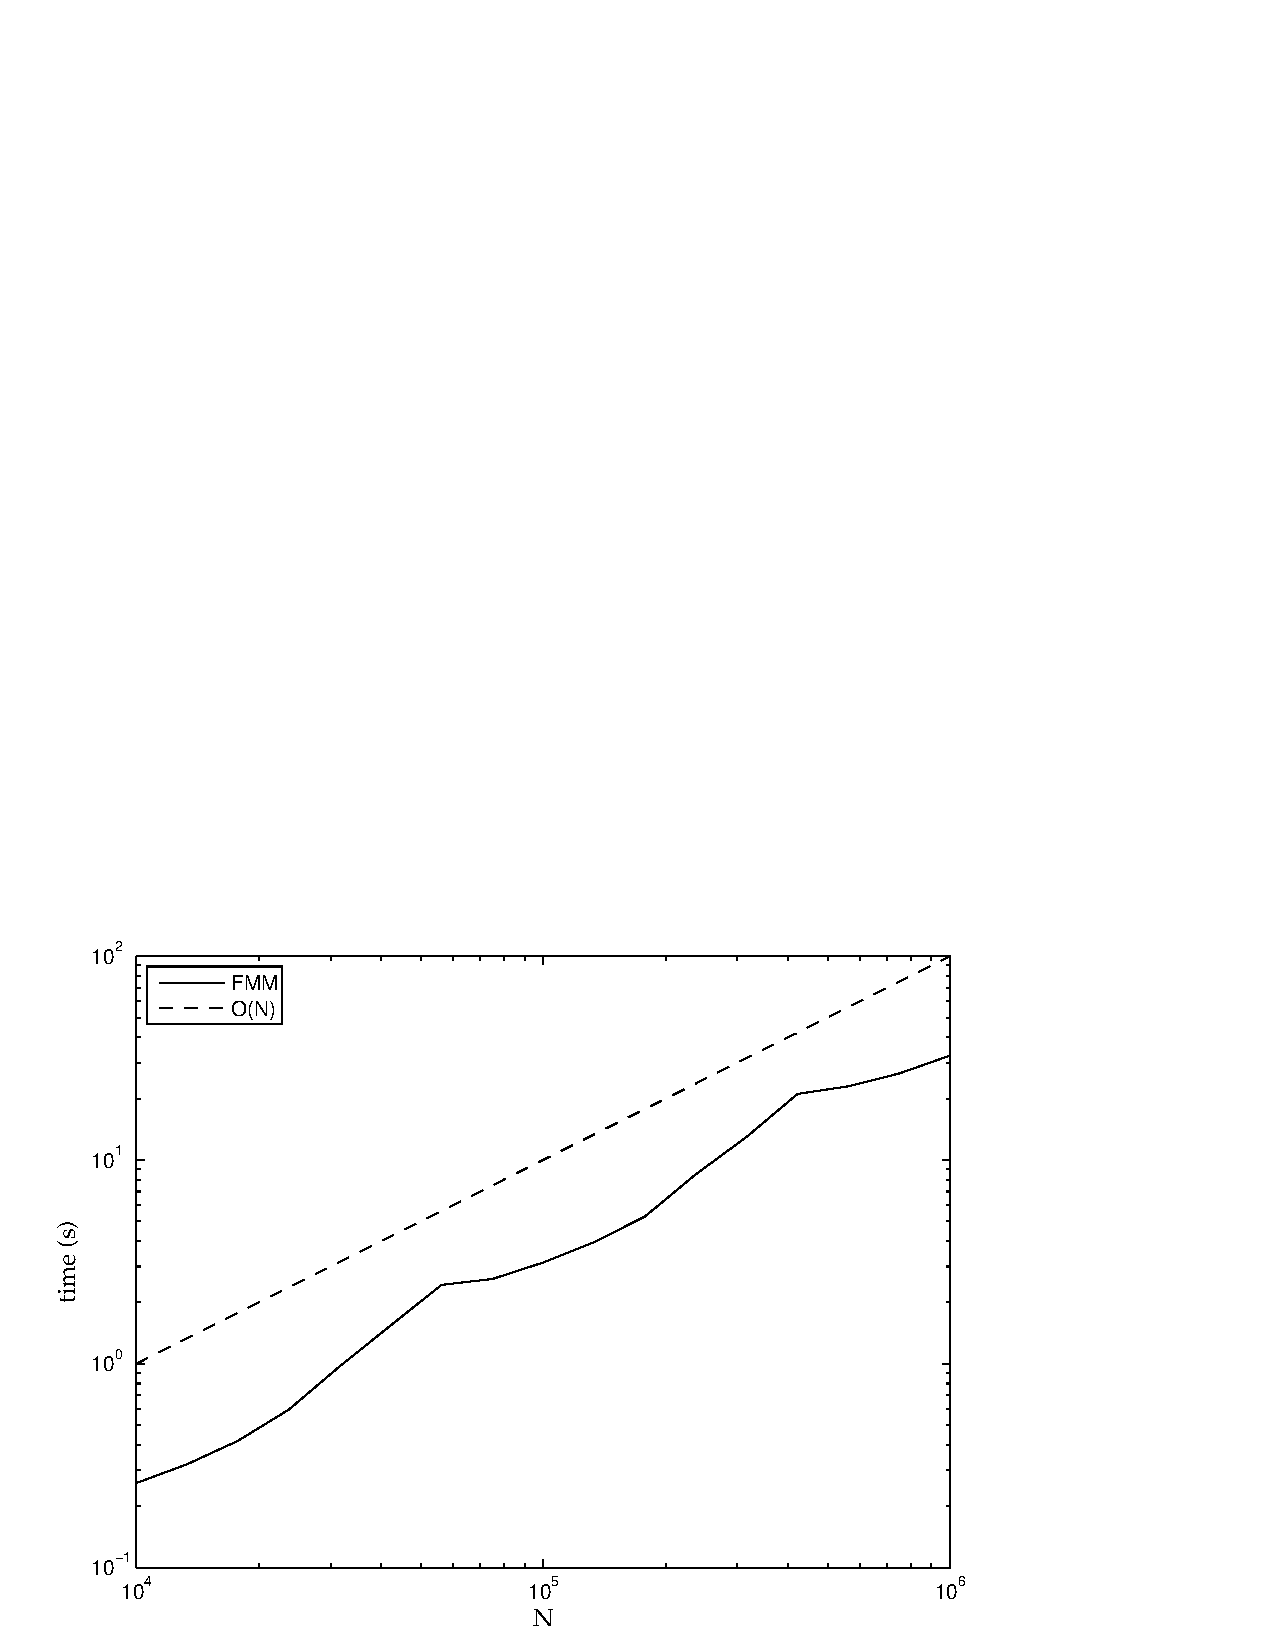
\includegraphics[width=14cm]{img/FMMScaling.pdf}
	\caption{Scaling of the {\fmm} with respect to problem size, $N$}
	\label{fig:fmm_scaling}
\end{center}
\end{figure}

This plot shows the overall scaling of the {\fmm} as $\O{N}$. The minor peaks are caused by the nature of the hierarchical decomposition -- when a new level is added it changes the balance of near and far-field computation, which is vital to the overall $\O{N}$ behavior. We could eliminate these peaks by tweaking $\ncrit$ for every test value of $N$, but the general trend of timing has already been shown.
\cleardoublepage

% -------------------------------------
% CHAPTER 5: LAPLACE
% -------------------------------------
%!TEX root = ../thesis.tex

\chapter{BEM with inexact GMRES for the Laplace equation}
\label{chapter:laplace_bem}
\thispagestyle{myheadings}

% set this to the location of the figures for this chapter. it may
% also want to be ../Figures/2_Body/ or something. make sure that
% it has a trailing directory separator (i.e., '/')!
\graphicspath{{Laplace/}}

To properly evaluate the utility of our relaxed {\fmm}-{\bem} method, we must apply it to a variety of examples, both to test for correctness (obtaining the correct answer and maintaining all convergence properties) and to evaluate the ``real-world'' potential for speedup.

% \section{Equation}\label{laplace:equation}

The first such example we will look at is the solution to Laplace's equation, consisting of obtaining $\phi(\vect{x})$ such that:

\begin{equation}\label{eqn:laplace}
	\nabla^{2}\phi(\vect{x}) = 0
\end{equation}

This equation can be used to model several applications, including electrostatics \cite{YokotaETal2010}, potential flow \cite{klaseboeretal2011} and heat transfer \cite{panti2008,majchrzakfreus2003}, and using {\fmmbem} in particular \cite{Nabors94}.

%By using the fundamental solution to \ref{eqn:laplace} we can write the potential at a point $\vect{x}_i$ from point $\vect{x}_j$ as a function of the distance between the two points,
%
%\begin{equation}\label{eqn:fundamental_laplace}
%	\phi(\vect{x}_i) = \frac{q_j}{|\vect{x}_i - \vect{x}_j|}.
%\end{equation}
%
%From the potential of a single pair of points, it is easy to find the influence from all points $\vect{x}_j,\; j=1..N$ at $\vect{x}_i$, as a simple $N$-body sum over \ref{eqn:fundamental_laplace}
%
%\begin{equation}
%	\phi(\vect{x}_i) = \sum_{j}^{N}\frac{q_j}{|\vect{x}_i - \vect{x}_j|}.
%\end{equation}
%
%These fundamental solutions, or Greens functions will be used later as part of the {\bem} formulation.

\section{BEM}\label{sec:bem_derivation}

To obtain a {\bem} formulation for Laplace, we start with the weak formulation of \ref{eqn:laplace}, with some weighting function, $W$,

\begin{equation}
	\int_{\Omega} \left [\nabla^{2}\phi\;W\right]\;\di{\Omega} = 0.
\end{equation}

We can write this in a different form,

\begin{equation}\label{eqn:laplace_weak_form}
	\int_{\Omega} \left [ \nabla(\nabla\phi\;W) - \nabla\phi\nabla W\right ] \;\di{\Omega} = 0.
\end{equation}

Applying Gauss' divergence theorem to the first term, we convert it into a surface integral, while simultaneous re-writing the second term, $\nabla\phi\nabla W = \nabla(\phi\nabla W) - \phi\nabla^{2}W$ gives us

\begin{equation}\label{eqn:laplace_bem_1}
	\int_{\Gamma}\left [ \nabla\phi\;W\cdot\nhat\right ]\;\di{\Gamma} - \int_{\Omega} \left [\nabla(\phi\nabla W) - \phi\nabla^{2}W\right ]\;\di{\Omega} = 0.
\end{equation}

Utilizing Gauss' divergence theorem once again, and choosing $W = G = 1/4\pi r$, the Green's function for the Laplace equation (while noting that $\nabla^{2}G = -\delta$), we obtain

\begin{equation}\label{eqn:laplace_bem_2}
	\int_{\Gamma}\partiald{\phi}{\nhat}G\;\di{\Gamma} - \int_{\Gamma} \phi\partiald{G}{\nhat}\;\di{\Gamma} - \int_{\Omega} \phi\nabla^{2}G\;\di{\Omega} = 0.
\end{equation}

Taking advantage of $\nabla^{2}G = -\delta$, we obtain the near-final form

\begin{equation}\label{eqn:laplace_bem_3}
	\int_{\Gamma}\partiald{\phi}{\nhat}G\;\di{\Gamma} - \int_{\Gamma} \phi\partiald{G}{\nhat}\;\di{\Gamma} - \phi = 0.
\end{equation}.

The final step we must perform is to take our target point, $i$, to the boundary, where we want to form a linear system. At $i$ we augment the domain by a small hemisphere around the point with radius $\epsilon$. We can then consider $i$ as $\epsilon \to 0$. The first integral to be treated is over $G$ as it presents a lower order singularity than the integral over $\partialdi{G}{\nhat}$.

\begin{eqnarray}
	\lim_{\epsilon\to0} \int_{\Gamma_\epsilon} G\partiald{\phi}{\nhat}\;\di{\Gamma} & = & \lim_{\epsilon\to0}\int_{\Gamma_\epsilon} \frac{1}{4\pi\epsilon}\partiald{\phi}{\nhat}\;\di{\Gamma} \\
	& = & \lim_{\epsilon\to0}\frac{2\epsilon^{2}}{4\pi\epsilon} \partiald{\phi}{\nhat} = 0
\end{eqnarray}

In a similar fashion, we take the integral over $\partialdi{G}{\nhat}$ to the surface,

\begin{eqnarray}
	\lim_{\epsilon\to0} \int_{\Gamma_\epsilon} \phi\partiald{G}{\nhat}\;\di{\Gamma} & = & -\lim_{\epsilon\to0} \int_{\Gamma_\epsilon} \phi\frac{1}{4\pi\epsilon^{2}} \\
	& = & -\lim_{\epsilon\to0} \phi\frac{2\pi\epsilon^{2}}{4\pi\epsilon^{2}} = -\frac{1}{2}\phi.
\end{eqnarray}

Utilizing these two results and applying them to equation \ref{eqn:laplace_bem_3} with some re-arrangement, we obtain the final form for the Laplace equation:

\begin{equation}\label{eqn:laplace_bem_final}
	\frac{1}{2}\phi + \int_{\Gamma} \phi\partiald{G}{\nhat}\;\di{\Gamma} = \int_{\Gamma}\partiald{\phi}{\nhat}G\;\di{\Gamma}.
\end{equation}

The constant of $1/2$ holds as long as target points are located on a smooth surface, that is to say, not on the edge or corner of a panel. As noted in \S\ref{sec:bem}, we use constant, flat panels with collocation, resulting in targets in the center of panels, allowing us to use this formulation with no changes.

%For a boundary element formulation for Laplace, we actually start from Poisson's equation, which will allow us to introduce any kind of additional sources, such as point charges, while setting $\vect{f} = 0$ recovers the standard Laplace's equation.
%
%\begin{equation}
%	\nabla^{2}\phi(\vect{x}) + \vect{f} = 0,
%	\label{eqn:poisson}
%\end{equation}
%
%\noindent
%Here $\vect{f} \in \R^{3}$ is a known function at all points. Next, we take the fundamental solution to \ref{eqn:poisson}, given by the greens function, $G = 1 / |\vect{x} - \vect{y}|$, which satisfies the relation
%
%\begin{equation}
%	\nabla^{2}G(\vect{x},\vect{y}) + \delta(\vect{x},\vect{y}) = 0,\;\;\forall \vect{x},\vect{y}\in\R^{3},
%	\label{eqn:greens_laplace}
%\end{equation}
%
%We now take Green's second identity
%
%\begin{equation}
%	\int_V \left ( u\nabla^{2}v - v\nabla^{2} u\right)\;\di{V} = \int_S \left ( u\partiald{v}{\nhat} - v\partiald{u}{\nhat} \right ) \;\di{S},
%	\label{eqn:greens_2nd_identity}
%\end{equation}
%
%\noindent
%setting $v = \phi$ and $u = G$, giving \ref{eqn:laplace_deriv_1}
%
%\begin{equation}
%	\begin{multlined}
%	\int_V \left (G(\vect{x},\vect{y})\nabla^{2}\phi(\vect{y}) - \phi(\vect{y})\nabla^{2}G(\vect{x},\vect{y}) \right ) \di{V} = \\ 
%	\int_S \left ( G(\vect{x},\vect{y})\partiald{\phi(\vect{y})}{\nhat} - \phi(\vect{y})\partiald{G(\vect{x},\vect{y})}{\nhat}\right ) \di{S}.
%	\end{multlined}
%	\label{eqn:laplace_deriv_1}
%\end{equation}
%
%Next, applying both \ref{eqn:poisson} and \ref{eqn:greens_laplace} to \ref{eqn:laplace_deriv_1} we get a general form for all $\vect{x} \in V$:
%
%\begin{equation}
%	\begin{multlined}
%	\phi(\vect{x}) = \int_S \left ( G(\vect{x},\vect{y})\partiald{\phi(\vect{y})}{\nhat} - \phi(\vect{y})\partiald{G(\vect{x},\vect{y})}{\nhat} \right ) \di{S}  \\
%	+ \int_V G(\vect{x},\vect{y})f(\vect{y}) \di{V}
%	\end{multlined}
%	\label{eqn:laplace_deriv_2}
%\end{equation}
%modified different form of \ref{eqn:laplace_deriv_2} with an additional constant, $c(\vect{x})$, determined by the position of $\vect{x}$ on a given element. Whenever the target is on a smooth part of the boundary, i.e. the center of a triangle in collocation schemes such as the one used in this work, $c(\vect{x}) = 1/2\;\forall\vect{x}\in S$
%
%%Starting from \ref{eqn:bem_1}, we set the test function, $w$ to be the Greens function for Laplace between two points, $G_{ij}$, \ref{eqn:fundamental_laplace}, giving us for collocation methods:
%
%%\begin{equation}
%%	0 = \int_{\Gamma}\partiald{\phi}{\nhat}G_{ij}\;\di{\Gamma} - \int_{\Gamma}\phi\partiald{G_{ij}}{\nhat}\;\di{\Gamma} + \int_{\Omega}\phi\nabla^{2}G_{ij}\;\di{\Omega}.
%%\end{equation}
%%
%%Using the identity $\nabla^{2}G_{ij} = -\delta_{ij}$, we finally get
%%
%%\begin{equation}
%%	\frac{1}{2}\phi = \int_{\Gamma}\partiald{\phi}{\nhat}G_{ij}\;\di{\Gamma} - \int_{\Gamma}\phi\partiald{G_{ij}}{\nhat}\;\di{\Gamma}.
%%\end{equation}
%
%Discretizing \ref{eqn:laplace_deriv_2} using collocation and setting $\vect{f} = 0\;\forall\vect{x}$,
%
%\begin{equation}
%	\frac{1}{2}\phi_i = \sum_j^{N} \int_{\Gamma}\partiald{\phi_j}{\nhat_j}G_{ij}\;\di{\Gamma_j} - \sum_j^{N} \int_{\Gamma}\phi_j\partiald{G_{ij}}{\nhat_j}\;\di{\Gamma_j}.
%\end{equation}

Finally, as we have specified constant elements, we can bring the $\phi_j$ and $\partialdi{\phi_j}{\hat{n}}$ terms outside their relevant integrals, and form the surface integrals as sums over discretized panels to give the final expression we will solve:

\begin{equation}
	\frac{1}{2}\phi_i = \sum_j^{N} \partiald{\phi_j}{\nhat_j}\;\int_{\Gamma}G_{ij}\di{\Gamma_j} - \sum_j^{N} \phi_j\int_{\Gamma}\partiald{G_{ij}}{\nhat_j}\;\di{\Gamma_j}.
\end{equation}

To find every $\phi_i$ and $\partialdi{\phi_i}{\nhat_i}$, we create a system of linear equations $A\vect{x}=\vect{b}$ where the elements $A_{ij}$ are given by:

\begin{equation}
	A_{ij} = 
	\begin{cases}
		\int_{\Gamma} G_{ij}\;\di{\Gamma_j}, & \phi\;\text{specified on panel}\;j \\
		\int_{\Gamma} \partiald{G_{ij}}{\nhat_j}\;\di{\Gamma_j}, & \partiald{\phi}{\nhat}\;\text{specified on panel } j
	\end{cases}
\end{equation}

\noindent
and $\vect{b}$ is formed from the known terms on the boundary -- for instance, if $\phi$ is specified on a panel $j$, then $\phi_j\int_{\Gamma_j}\partialdi{G_{ij}}{\nhat_j}\;\di{\Gamma_j}$ will be added to $b_i$. 

Expanding out these operators into the actual forms of $G_{ij}$ and $\partialdi{G_ij}{\nhat_j}$ we obtain expressions in terms of $1/r$ and $\nhat_j\cdot\nabla(1/r)$.

\begin{eqnarray}
	\label{eqn:laplace_bem_G}\int_{\Gamma} G_{ij}\;\di{\Gamma_j} & = & \int_{\Gamma} \frac{1}{|\vect{x}_i-\vect{x}_j|} \;\di{\Gamma_j} \\ 
	\label{eqn:laplace_bem_dGdn}\int_{\Gamma} \partiald{G_{ij}}{\nhat_j}\;\di{\Gamma_j} & = & \int_{\Gamma}\frac{d\vect{x}\cdot\nhat_j}{|\vect{x}_i-\vect{x}_j|^{3}}\;\di{\Gamma_j}
\end{eqnarray}

Exactly how to evaluate these integrals numerically has been discussed in detail in \S\ref{subsec:numerical_integration}, so we just need to deal with the final details of our scheme -- the far-field approximations used for the {\fmm}.

\section{Expansions}\label{sec:laplace_expansions}

While there are many different ways to approximate the Laplace Green's function, we  choose to use spherical harmonics due to their superior scaling at high values of $p$ (translations such as \mtol scale as $\O{p^{4}}$ instead of $\O{p^{6}}$ for cartesian expansions). This choice of expansion will give us distinct multipole (singular) and local (regular) representations, convergent in different parts of the domain.

Remember that the potential at a point $\vect{x}_i$ from $N$ sources, $\vect{x}_j$, denoted here (to avoid clashing with the spherical co-ordinate $\phi$) by $\Phi(\vect{x}_i)$ is given by

\begin{equation}
	\Phi(\vect{x}_i) = \sum_{j=0}^{N} \frac{q_j}{|\vect{x}_i - \vect{x}_j|}
	\label{eqn:laplace_initial}
\end{equation}

We begin by taking two points, $\vect{x}_i, \; \vect{x}_j \in \R^{3}$, and an intermediate point between them, $\vect{x}_*$. Next, we look at the pair of vectors, $\vect{x}_i - \vect{x}_* = \vect{x}_{i*}$ and $\vect{x}_j - \vect{x}_* = \vect{x}_{j*}$ in spherical coordinates.
\begin{eqnarray*}
	\vect{x}_{i*} & = & \vect{x}_{i*}(r, \theta, \phi) \\
	\vect{x}_{j*} & = & \vect{x}_{j*}(\rho, \alpha, \beta)
\end{eqnarray*}

If we let $\gamma$ be the angle between $\vect{x}_{i*}$ and $\vect{x}_{j*}$, we can write the distance between these two points, $r'$ as

\begin{equation}
	r'^{2} = r^{2} + \rho^{2} - 2r\rho\cos\gamma,
\end{equation}

\noindent
where $\cos\gamma = \cos\theta\cos\alpha + sin\theta\sin\alpha\cos(\phi-\beta)$. By setting $\mu = \rho / r$ and $u = \cos\gamma$ we directly write

\begin{equation}
	\frac{1}{r'} = \frac{1}{r\sqrt{1-2u\mu + \mu^{2}}}.
\end{equation}

For $\mu > 1$ we can expand $1/r'$ in terms of $\mu^{n}$, resulting in a Legendre polynomial of order $n$, given by

\begin{equation}
	\frac{1}{\sqrt{1-2u\mu + \mu^{2}}} = \sum_{n=0}^{\infty}P_n(u)\mu^{n},
\end{equation}

\noindent
and so we can write our expression for $1/r'$ as

\begin{equation}
	\frac{1}{r'} = \sum_{n=0}^{\infty} \frac{\rho^{n}}{r^{n+1}}P_n(u).
	\label{eqn:laplace_2}
\end{equation}

It is worth noting that our expansion is still coupled in terms of $\vect{x}_i$ and $\vect{x}_j$, so we use the ``well-known'' result \cite{stegun1964} that Legendre polynomials can be expressed in terms of spherical harmonics

\begin{equation}
	P_n(u) = \frac{4\pi}{2n+1}\sum_{m=-n}^{n}Y^{-m}_n(\alpha, \beta)Y^{m}_n(\theta, \phi),
	\label{eqn:laplace_3}
\end{equation}

\noindent
with

\begin{equation}
	Y^{m}_n(\theta, \phi) = \sqrt{\frac{2n+1}{4\pi}}\sqrt{\frac{(n-|m|)!}{(n+|m|)!}}P^{|m|}_n(\cos\theta)e^{im\phi}.
\end{equation}

In this form for $Y^{m}_n$, the associated Legendre polynomials, $P^{m}_n$ must be calculated using Rodrigues' formula \cite{Rodrigues1815}

\begin{equation}
	P_n(x) = \frac{1}{2^{n}n!}\frac{\text{d}}{\text{d}x^{n}}(x^{2}-1)^{n}
\end{equation}

By combining equations \ref{eqn:laplace_initial}, \ref{eqn:laplace_2} and \ref{eqn:laplace_3}, we get two very similar forms

%In the followi ng equations, $M^{m}_n$ are the multipole coefficients, and $L_n^{M}$ the local coefficients. In each case we represent sources and targets in spherical co-ordinates, with: $\vect{x}_i = (r_i, \theta_i, \phi_i)$ and $\vect{x}_j = (\rho_j, \alpha_j, \beta_j)$.

\begin{eqnarray}
	\Phi(\vect{x}_i) & = & \sum_{n=0}^{p}\sum_{m=-n}^{n}\frac{Y^{m}_n(\theta_i,\phi_i)}{r_i^{n+1}}\underbrace{\left \{ \sum_j^{N}q_j\rho^{n}_jY^{-m}_n(\alpha_i,\beta_i)\right \} }_{M^{m}_n} \\
	\Phi(\vect{x}_i) & = & \sum_{n=0}^{p}\sum_{m=-n}^{n}r_i^{n}Y^{m}_n(\theta_i,\phi_i)\underbrace{\left \{ \sum_j^{N}q_j\frac{Y^{-m}_n(\alpha_i,\beta_i)}{\rho^{n+1}_j}\right \} }_{L^{m}_n},
\end{eqnarray}

\noindent
with $M^{m}_n$ and $L^{m}_n$ as the multipole (singular) and local (regular) coefficients respectively.

While the approximation of $G = 1/4\pi r$ is easy with the {\fmm}, forming multipole expansions for $\partialdi{G}{\nhat}$ requires a little more work. Working from $\partialdi{G}{\nhat} = \nabla G\cdot\nhat$, to form the desired multipole expansion requires the computation of $\partialdi{M^{m}_n(r,\theta,\phi)}{\nhat}$. Taking each derivative in turn, and initially working in spherical coordinates,

\begin{eqnarray}
	\di{r} & = & \frac{n}{r}M^{m}_n \nonumber \\
	\di{\theta} & = & r^{n}\partiald{Y^{m}_n(\theta,\phi)}{\theta} \nonumber \\
	\di{\varphi} & = & -imM^{m}_n. \nonumber
\end{eqnarray}

We can now use a simple conversion into cartesian coordinates in order to perform the dot product with $\nhat$:

\begin{equation*}
	\left(\begin{array}{c}
		\di{x} \\
		\di{y} \\
		\di{z}
	\end{array}\right) = 
	\left(\begin{array}{ccc}
		\sin{\theta}\sin{\phi} & (\cos{\theta}\cos{\phi})/r & -(\sin{\theta}\sin{\phi})/r \\
		\sin{\theta}\sin{\phi} & (\cos{\theta}\sin{\phi})/r & (\sin{\theta}\cos{\phi})/r \\
		\cos{\theta} & -(\sin{\theta})/r & 0
	\end{array}\right) \cdot \left(\begin{array}{c}
		\di{r} \\
		\di{\theta} \\
		\di{\phi}
	\end{array}\right)
\end{equation*}

To translate and convert these expansions, we reproduce without proof the formulae from \cite{greengard1987} for multipole-multipole (\ref{eqn:laplace_spherical_m2m}), multipole-local (\ref{eqn:laplace_spherical_m2l}) and local-local translations (\ref{eqn:laplace_spherical_l2l}), where $A^{m}_n = (-1)^{n}/(n-m)!(n+m)!$.

\begin{eqnarray}
	\label{eqn:laplace_spherical_m2m}
	M^k_j & = & \sum_{n=0}^j \sum_{m=-n}^n \frac{\hat{M}^{k-m}_{j-n}i^{|k|-|m|-|k-m|}A^m_nA^{k-m}_{j-n}\rho^nY^{-m}_n(\alpha,\beta)}{(-1)^nA^k_j} \;\;\;\;\text{(M2M)}\\
	& & \nonumber \\
	\label{eqn:laplace_spherical_m2l}
	L^k_j & = & \sum_{n=0}^j \sum_{m=-n}^n \frac{M^{m}_{n}i^{|k-m|-|k|-|m|}A^m_nA^{k}{j}Y^{m-k}_{j+n}(\alpha,\beta)}{(-1)^{j+k}A^{m-k}_{j+n}\rho^{j+n+1}} \;\;\;\;\text{(M2L)}\\
	& & \nonumber \\
	\label{eqn:laplace_spherical_l2l}
	L^k_j & = & \sum_{n=0}^j \sum_{m=-n}^n \frac{\hat{L}^{m}_{n} i^{|m|-|k|-|m-k|}A^{m-k}_{n-j}A^{k}_{j}\rho^{n-j}Y^{m-k}_{n-j}(\alpha,\beta)}{A^{m}_{n}}\;\;\;\;\text{(L2L)}.
\end{eqnarray}

We note that there are more efficient versions of these translations, for instance, factorized translation operators that rely on the ability to rotate spherical harmonics to a chosen orientation -- this would allow all $Y^{m}_n(\alpha,\beta)$ terms in equations \ref{eqn:laplace_spherical_m2m}-\ref{eqn:laplace_spherical_l2l} to be replaced with $Y^{m}_n(0,0)$, which can be precomputed. At the cost of extra memory for precomputed values, this reduces the cost from $\O{p^{4}}$ to $\O{p^{3}}$ \cite{GreengardRokhlin1997}. Further algorithmic gains can be made using a plane wave expansion formulation for the {\mtol} operator, where we convert multipoles into plane waves ($\O{p^{3}}$), translate them ($\O{p^{2}}$) and finally convert them back into local expansions ($\O{p^{3}}$). This method keeps the overall complexity of the {\mtol} at $\O{p^{3}}$, but with lower constant terms \cite{GreengardRokhlin1997}.

%%%%% CONVERGENCE
\section{Convergence}\label{sec:laplace_convergence}

As an initial test of our {\fmm}-{\bem} implementation, we wish to verify its convergence to a known solution based on the spatial resolution of our mesh. To do this,  we use simple tests of constant potential and charge on the surface of a sphere. We use the analytical solution of $\phi = \partialdi{\phi}{\nhat} = 1$. The presence of an analytical solution makes this problem perfect for convergence testing for both 1st-kind (solving for $\phi$ with $\partialdi{\phi}{\nhat}$ known) and 2nd-kind (solving for $\partialdi{\phi}{\nhat}$ with $\phi$ known). The geometry is produced by forming an initial approximation for the sphere using 8 triangles, then recursively splitting each triangle into 4 smaller panels. In this way we can control the spatial discretization of the geometry and use it to test real-world convergence of our {\bem} for both first and second-kind equations. Two examples of the spherical domain are shown in figures \ref{fig:sphere128} and \ref{fig:sphere2048}.

\begin{center}
\begin{figure}[h]
	\subfloat[][128 panels]{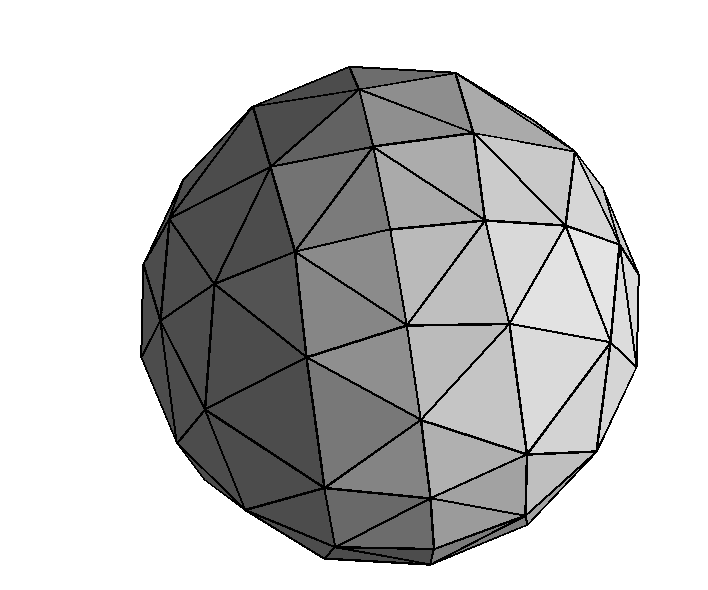
\includegraphics[width=7.5cm]{img/sphere128.pdf}\label{fig:sphere128}}\qquad
	\subfloat[][2048 panels]{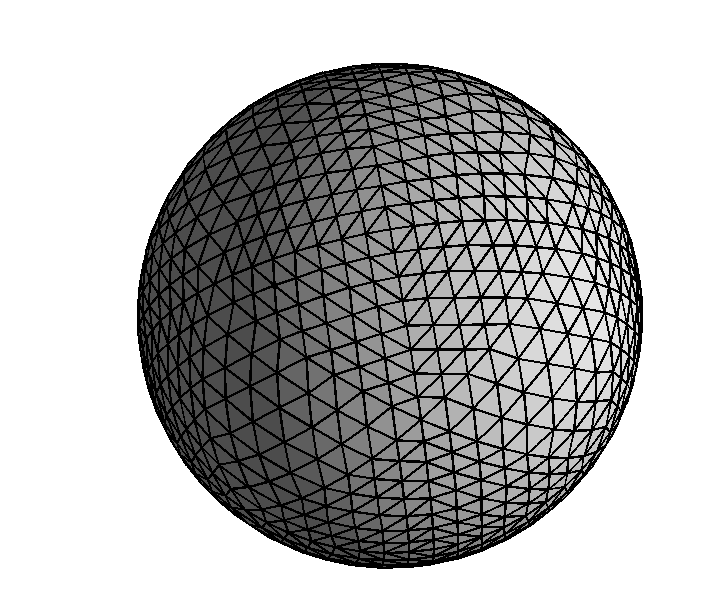
\includegraphics[width=7.5cm]{img/sphere2048.pdf}\label{fig:sphere2048}}\qquad
	\caption{Triangular discretizations of a sphere}
	\label{fig:glob_spheres}
\end{figure}
\end{center}

All tests were performed using a canonical right-preconditioned {\gmres} (algorithm \ref{alg:gmres}) implementation, using our \lstinline|FMM_Plan| framework (see appendix \ref{chapter:fmm_plan}) for the matrix-vector products. We used spherical harmonic expansions for the far-field, and the semi-analytical integral described in \S\ref{subsubsec:semi_analytical} for singular integrals. High precision Gauss quadrature was used for near-singular integrals. In all cases, $\theta_{\text{MAC}} = 0.5$, $p = 10$ and a solver tolerance of $10^{-6}$ was used in order to minimize all but discretization errors.

% Given that the spatial convergence of the collocation method for {\bem} has not been analytically proven, it is important to show that our method behaves as expected. Figures \ref{fig:spatial_convergence_1st} and \ref{fig:spatial_convergence_2nd} show the spatial convergence of the {\fmm}-{\bem} solving  for $\partialdi{\phi}{\hat{n}}$ and $\phi$ respectively. 
%
%\begin{center}
%\begin{figure}[htbp]
%	\subfloat[][1st-kind equation]{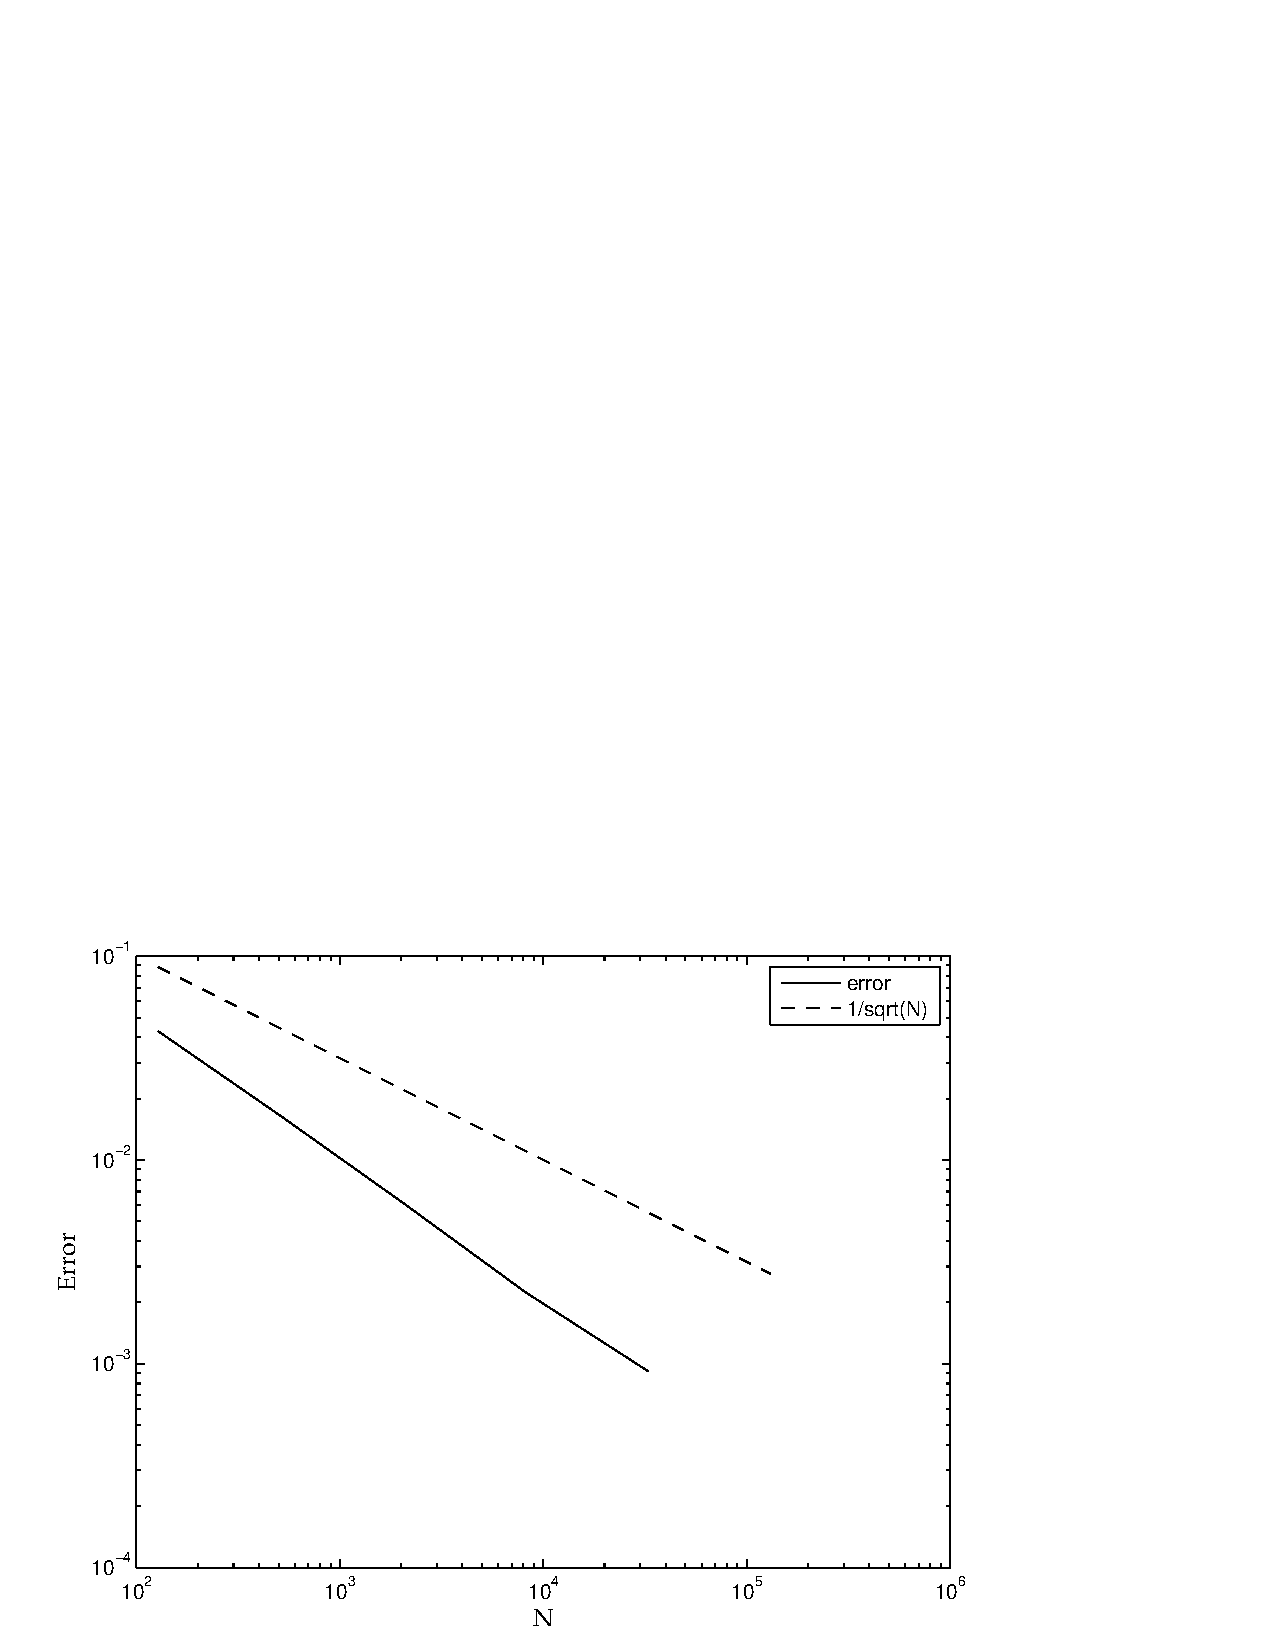
\includegraphics[width=7.5cm]{img/first_kind_convergence.pdf}\label{fig:spatial_convergence_1st}}
%	\subfloat[][2nd-kind equation]{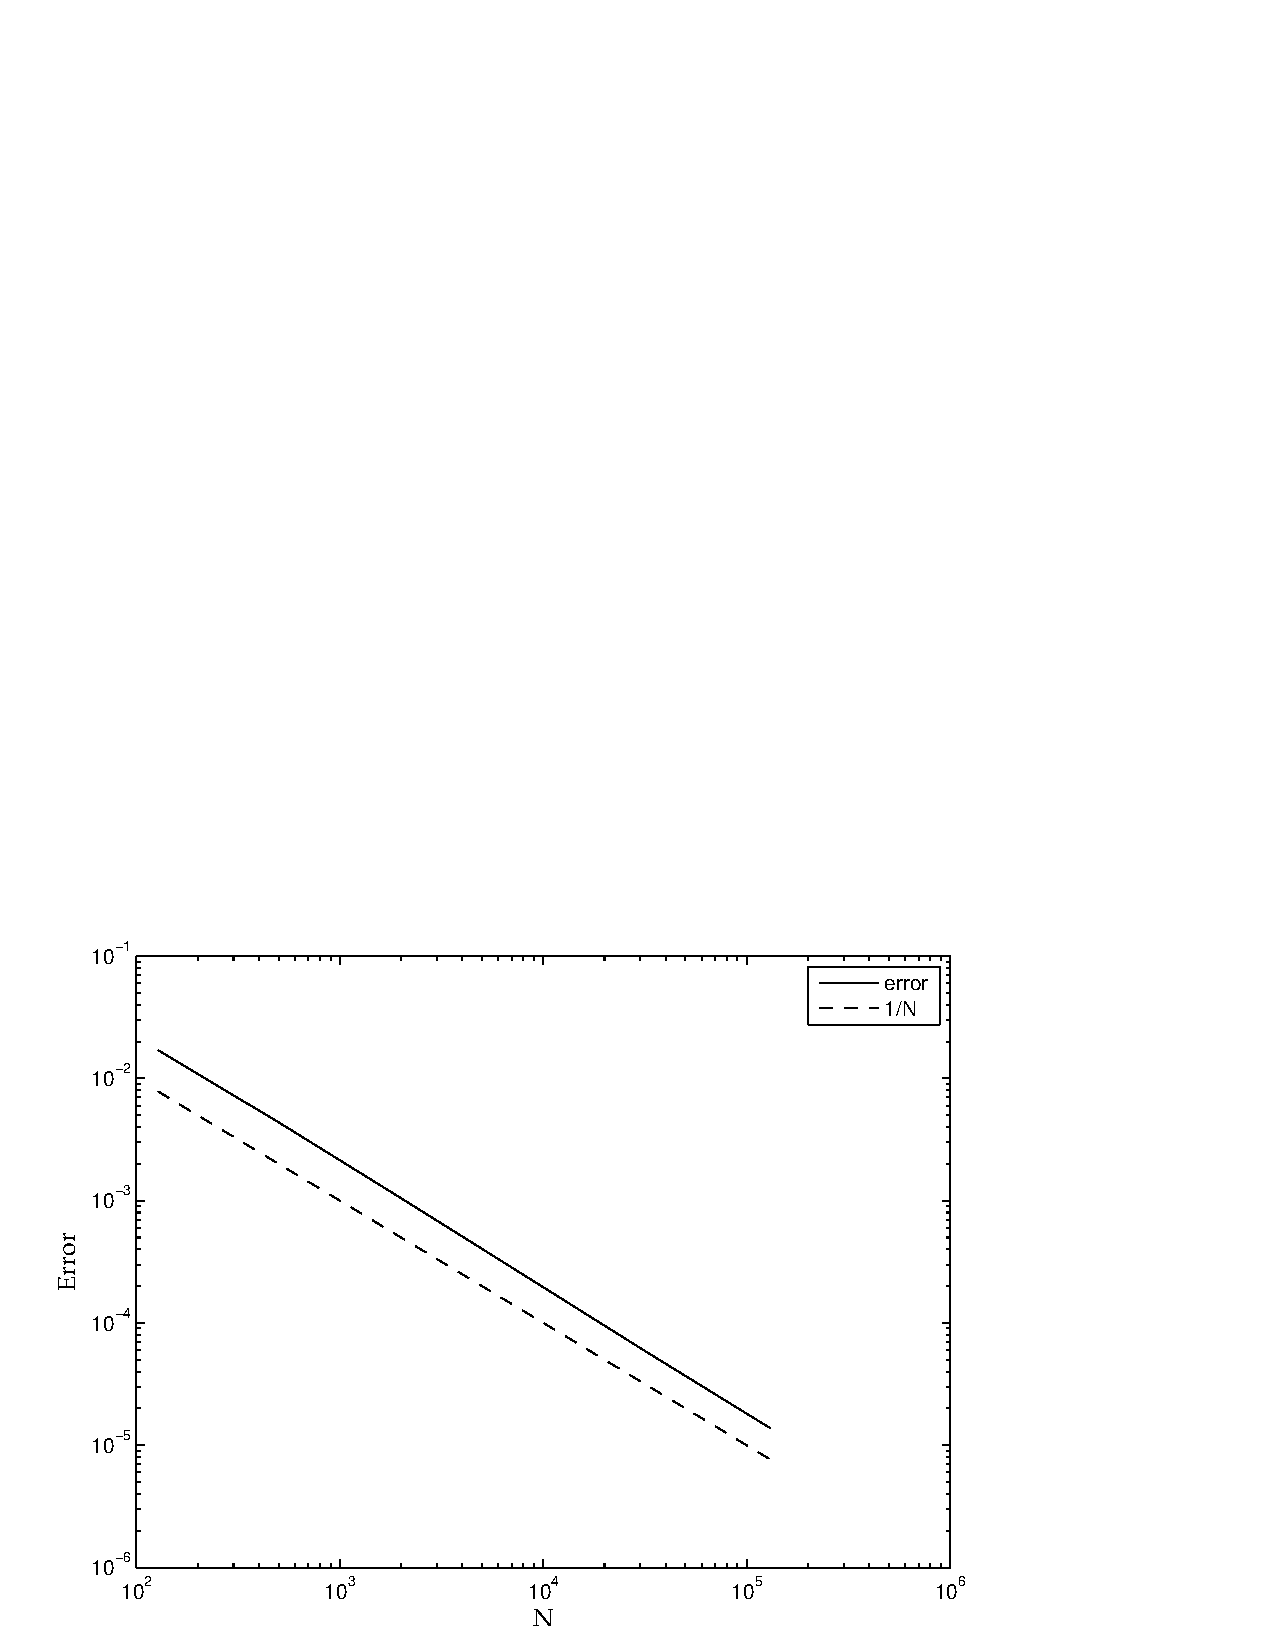
\includegraphics[width=7.5cm]{img/second_kind_convergence.pdf}\label{fig:spatial_convergence_2nd}}
%	\caption{Spatial converge of 1st and 2nd-kind solves}
%	\label{fig:glob_convergence}
%	
%\end{figure}
%\end{center}

\begin{figure}[h]
\begin{center}
	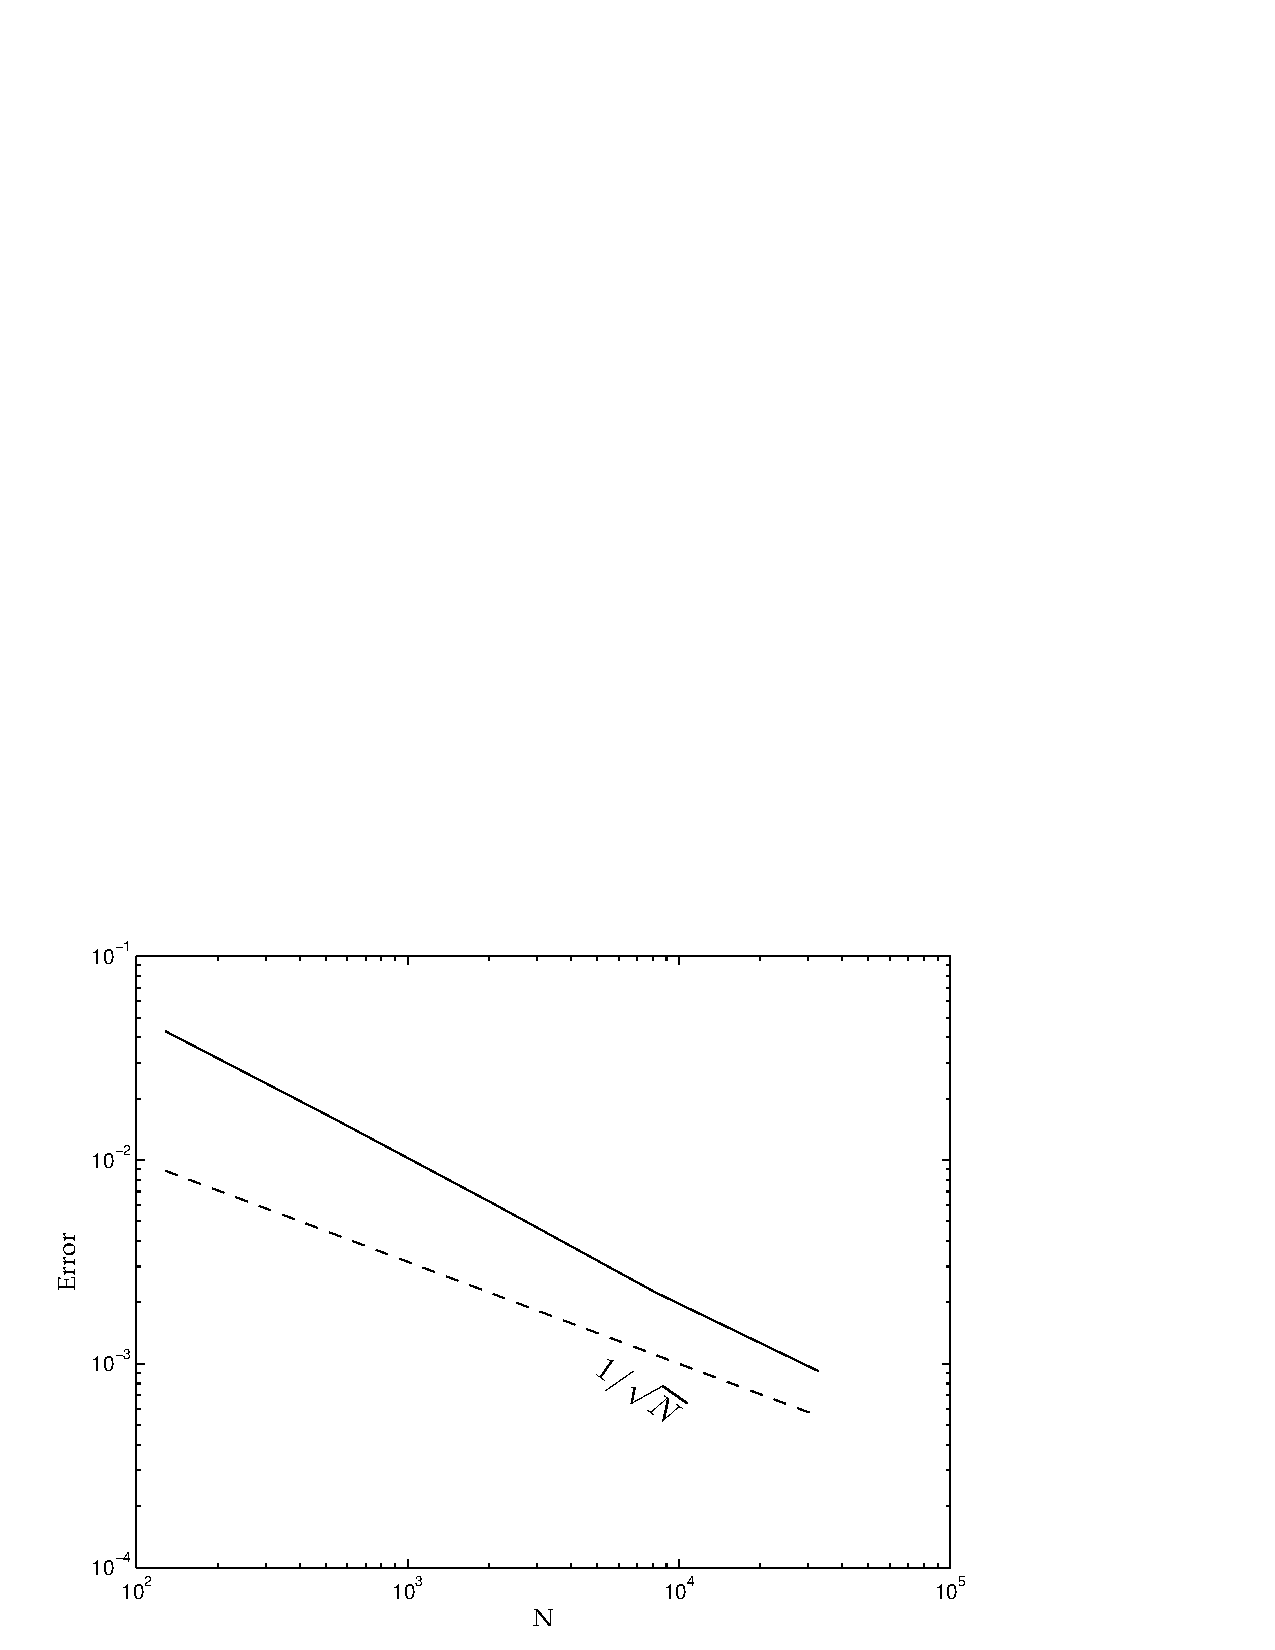
\includegraphics[width=14cm]{img/FirstKindConvergence.pdf}
	\caption{Convergence of 1st-kind solve for Laplace equation on a sphere, solving with $p=10$, solver tolerance of $10^{-6}$.}
	\label{fig:laplace_1st_convergence}
\end{center}
\end{figure}

\begin{figure}[h]
\begin{center}
	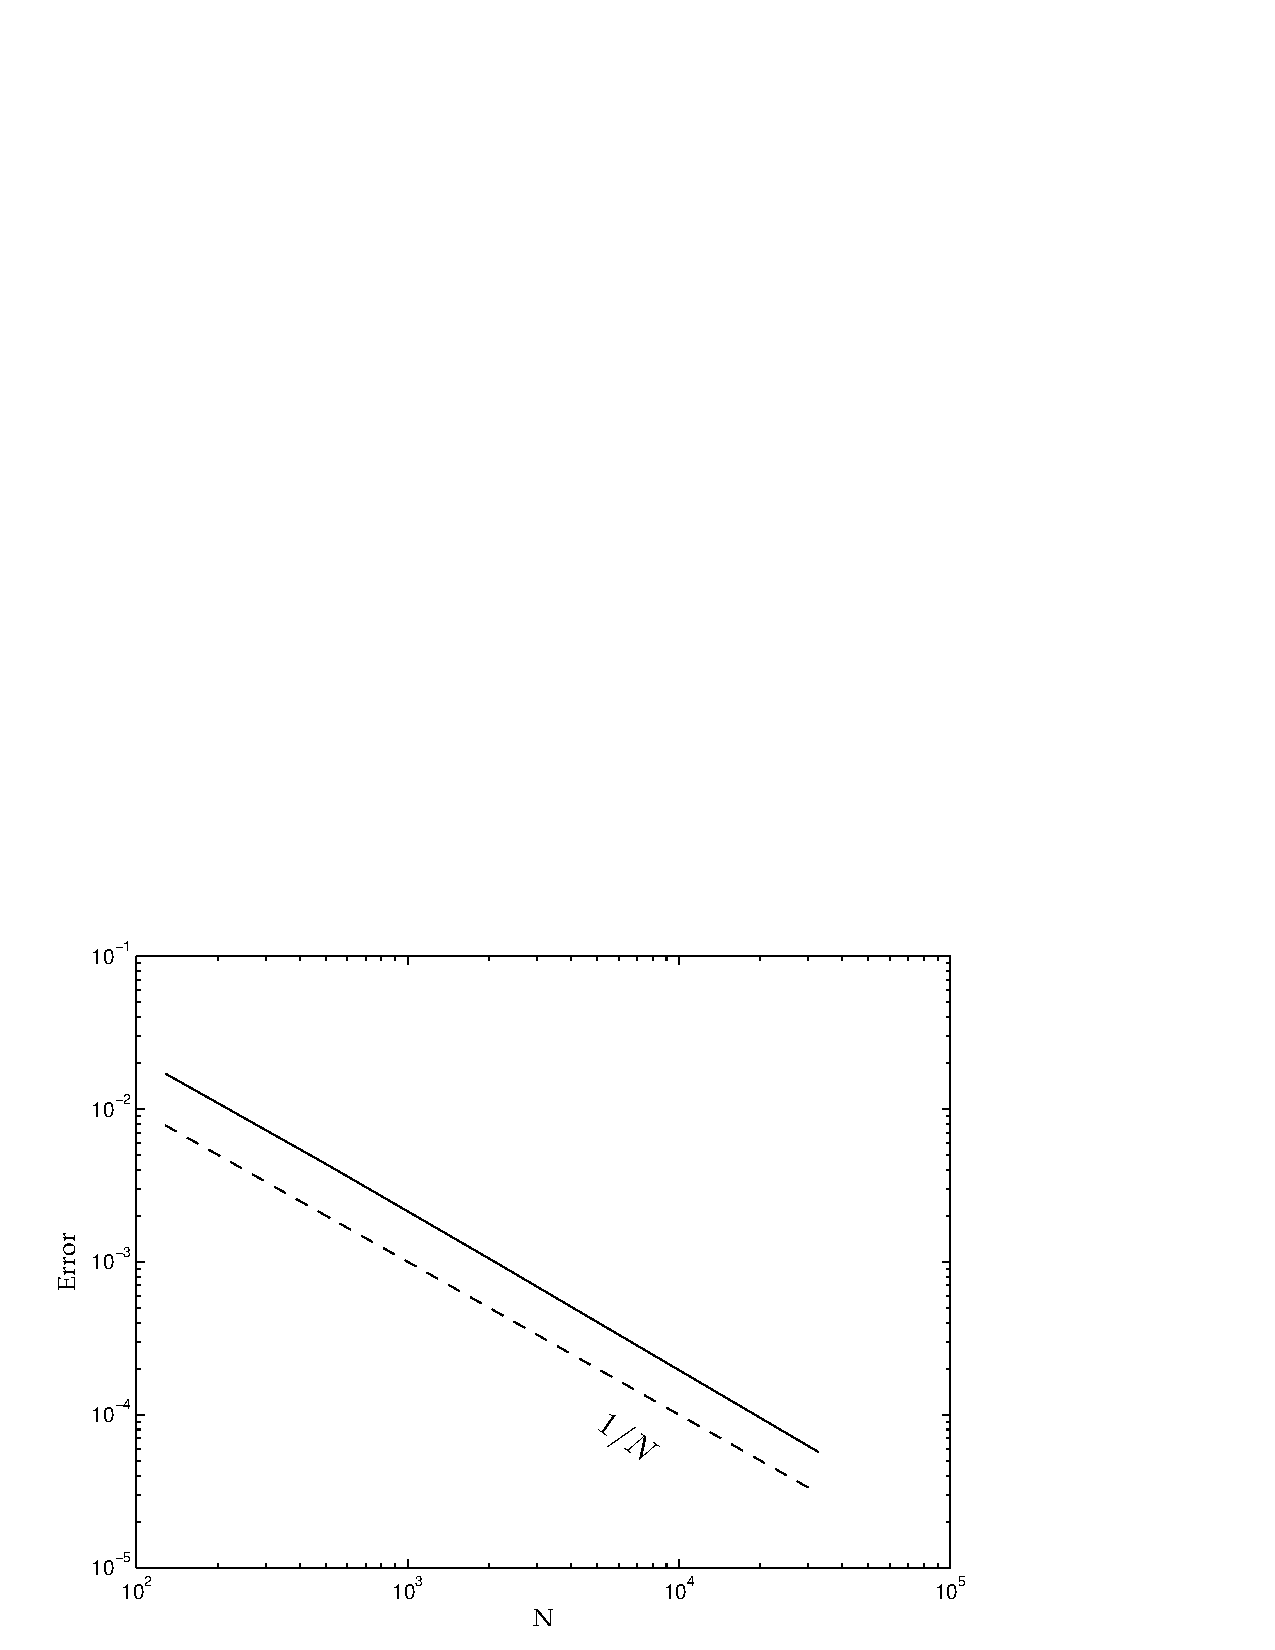
\includegraphics[width=14cm]{img/SecondKindConvergence.pdf}
	\caption{Converge of 2nd-kind solve for Laplace equation on a sphere, solving with $p=10$, solver tolerance of $10^{-6}$.}
	\label{fig:laplace_2nd_convergence}
\end{center}
\end{figure}

Figures \ref{fig:laplace_1st_convergence} and \ref{fig:laplace_2nd_convergence} are encouraging, as they display the correct orders of convergence that we expect compared to comparable codes, namely $\O{1/N}$ for the 2nd-kind solve, while achieving slightly better than $\O{1/\sqrt{N}}$ in the 1st-kind solve. This implies that our {\bem} formulation is correct, the singular / near-singular integrals are accurate, and the far-field approximation using the {\fmm} is also giving the expected answer. This provides the basis we will use to continue experimenting with our code, and ensures that when we use relaxed solvers, we can test their convergence, and be sure that we are still getting the correct answer.

%%%%%%%%%%%%%%%%%%%%%%%%%%%%%%%%%
%%%%% RELAXATION
%%%%%%%%%%%%%%%%%%%%%%%%%%%%%%%%%
\section{Relaxation}\label{sec:laplace_relaxation}

We are trying to minimize the time taken to solve {\bem} problems while not sacrificing accuracy, so it is vital to see how the modifications affect our code's behavior. First, we look at an example problem and see how the residual changes with {\gmres} iterations, and the $p$ required to continue convergence.

\begin{figure}[h]
	\centering
	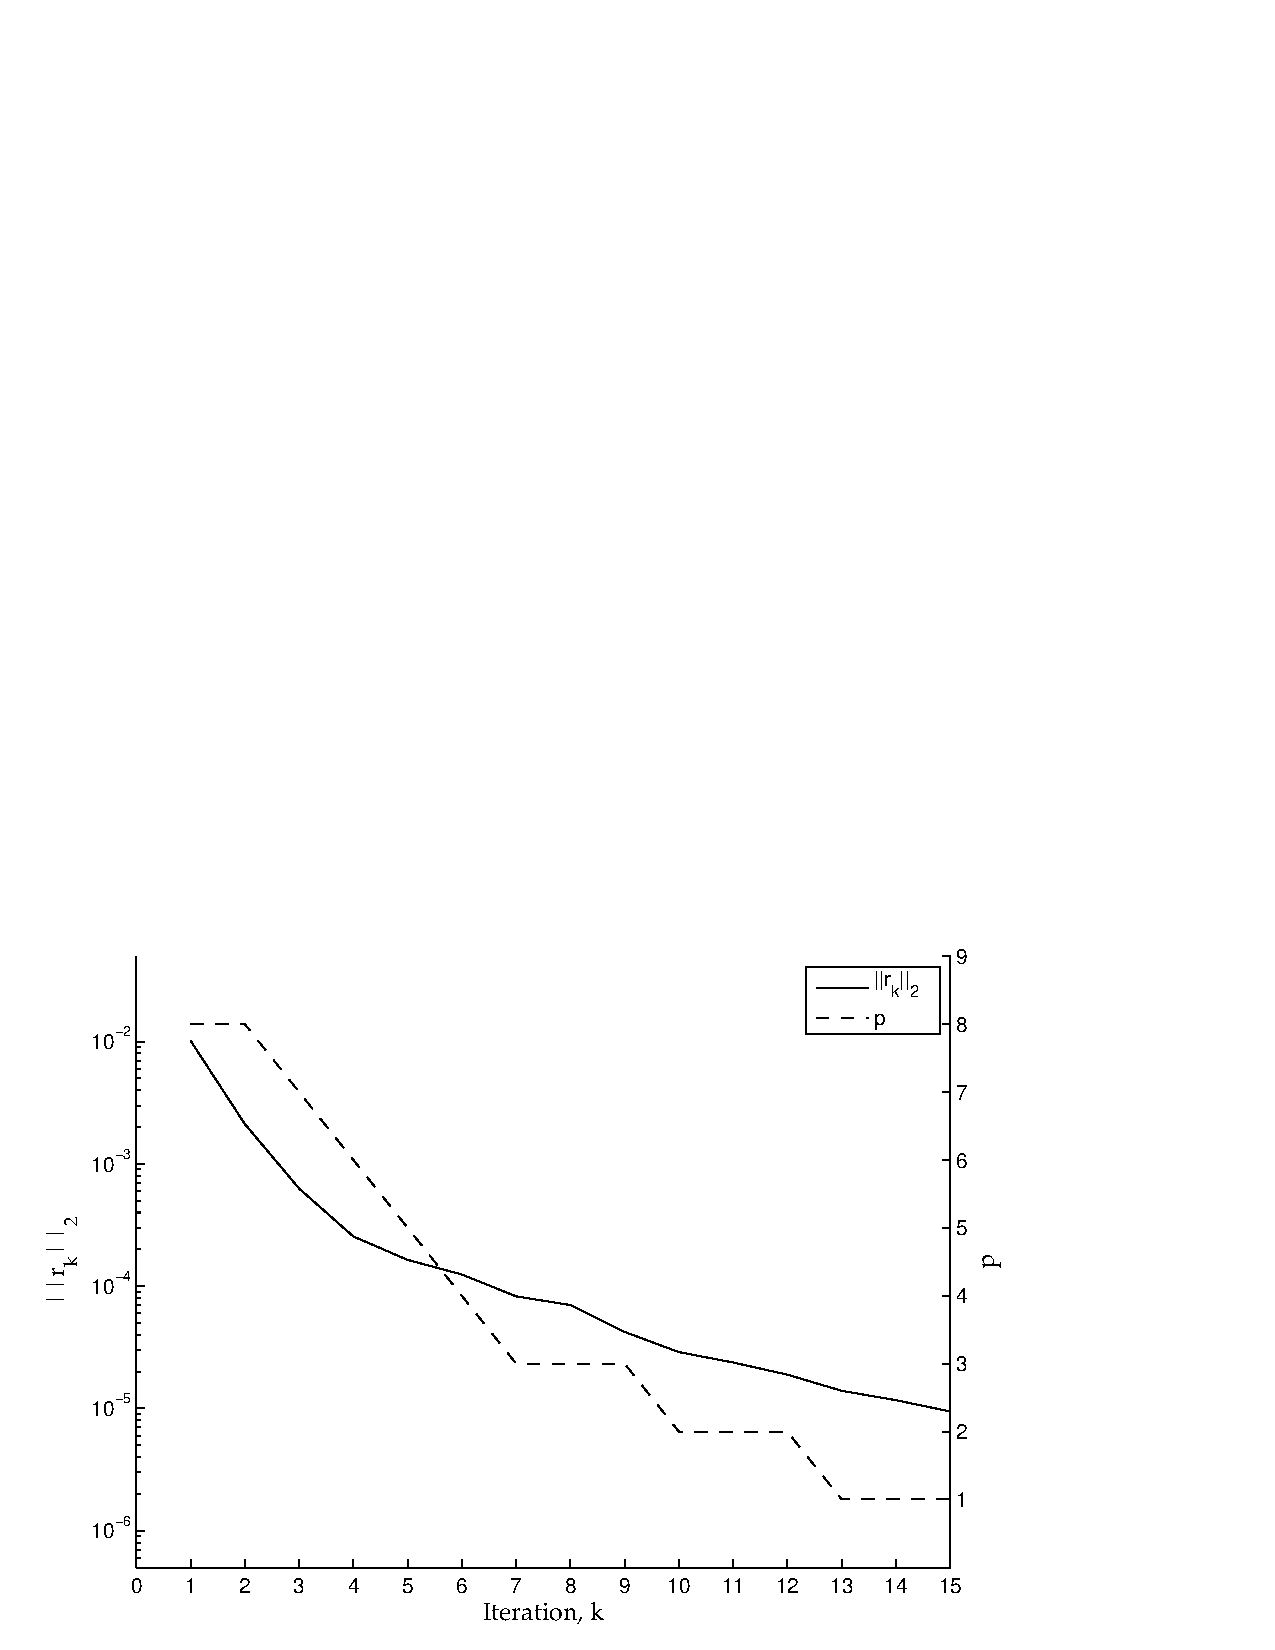
\includegraphics[width=14cm]{img/resid_p_iteration.pdf}
	\caption{Behaviour of the residual $||r_{k}||$ and necessary $p$ against {\gmres} iteration number}
	\label{fig:residualp}
\end{figure}

Figure \ref{fig:residualp} shows how both $||r_{k}||$ and $p$ change over the course of a solve. In this problem, 32768 panels were used to solve the first-kind equation on a sphere to a tolerance of $10^{-5}$ with an initial $p$ set to 8. Clearly, as the residual drops, the $p$ required to maintain convergence of the solver drops significantly, down from $p=8$ at the first iteration to $p=3$ at the 7th. Kernel translation operators in this implementation scale from $\bigO(p^{4})$ for spherical harmonics to $\bigO(p^{6})$ for Cartesian kernels, thus this drop in $p$ can result in large savings in terms of the work being performed. % performance gains.

Next, we compare problems with and without a relaxation strategy. Figure \ref{fig:relaxation_timing} shows the results of tests from 8192 to 131072 panels with a solver tolerance of $10^{-5}$ using a multi-threaded evaluator on 4 cores. For all experiments in this section $\ncrit$ was chosen for each test to minimize the solution time. Only the time spent solving $Ax=b$, $\tsolve$ is plotted. While there are many metrics that could be used to establish performance, we choose to use time-to-solution in all cases for the following reasons:

\begin{enumerate}
\item Reporting times normalized on the number of iterations will both show the same speedups (due to the identical number of iterations required for relaxed and fixed-$p$ solvers), and show exactly the same speedups as the total time-to-solution.

\item Times, rather than operation counts (whether total or per-iteration) are used to abstract away as much as possible the implementation details --- we could potentially use a ``reference operations'' count, the operations required to perform a direct ($\O{N^{2}}$ solve), normalized by either total time (operations per second) or by iterations (average operations per second per iteration), but neither of these options provide any real advantage to simply reporting times.

\item Showing times / operation counts for individual iterations is too unwieldy --- instead of presenting a single value of speedup for each experiment, either multiple values (up to 70+ iterations in some of the later experiments in this thesis) or a plot would need to be presented.
\end{enumerate}

\begin{table}[h]
\begin{center}
\begin{tabular}{c|cc|cc|c}
  & \multicolumn{2}{c|}{Non-Relaxed} & \multicolumn{2}{c|}{Relaxed} & \\
  N & $\ncrit$ & $\tsolve$ & $\ncrit$ & $\tsolve$ & Speedup \\
   & & & & & \\ \hline
   & & & & & \\
  2048 & 400 & 0.27 & 200 & 0.40 & 0.675 \\
   & & & & & \\
  8192 & 400 & 2.58 & 200 & 1.7 & 1.52 \\
   & & & & & \\
  32768  & 400 & 7.1 & 200 & 5.07 & 1.40 \\
   & & & & & \\
  131072  & 400 & 30.1 & 200 & 20.72 & 1.45 \\
 
\end{tabular}
\end{center}
\caption{Speedups for Laplace 1st-kind relaxation, $p=8$, solver tolerance of $10^{-5}$}
\label{tab:laplace_1st_relaxation}
\end{table}%

\begin{table}[h]
\begin{center}
\begin{tabular}{c|cc|cc|c}
  & \multicolumn{2}{c|}{Non-Relaxed} & \multicolumn{2}{c|}{Relaxed} & \\
  N & $\ncrit$ & $\tsolve$ & $\ncrit$ & $\tsolve$ & Speedup \\
   & & & & & \\ \hline
   & & & & & \\
  2048 & 400 & 0.13 & 200 & 0.64 & 0.20 \\
   & & & & & \\
  8192 & 400 & 1.49 & 200 & 1.19 & 1.25 \\
   & & & & & \\
  32768 & 400 & 6.77 & 200 & 5.92 & 1.14 \\
   & & & & & \\
  131072 & 400 & 30.01 & 200 & 24.2 & 1.24 \\
 
\end{tabular}
\end{center}
\caption{Speedups for Laplace 2nd-kind relaxation, $p=8$, solver tolerance of $10^{-5}$}
\label{tab:laplace_2nd_relaxation}
\end{table}%

\begin{figure}[h]
	\centering
	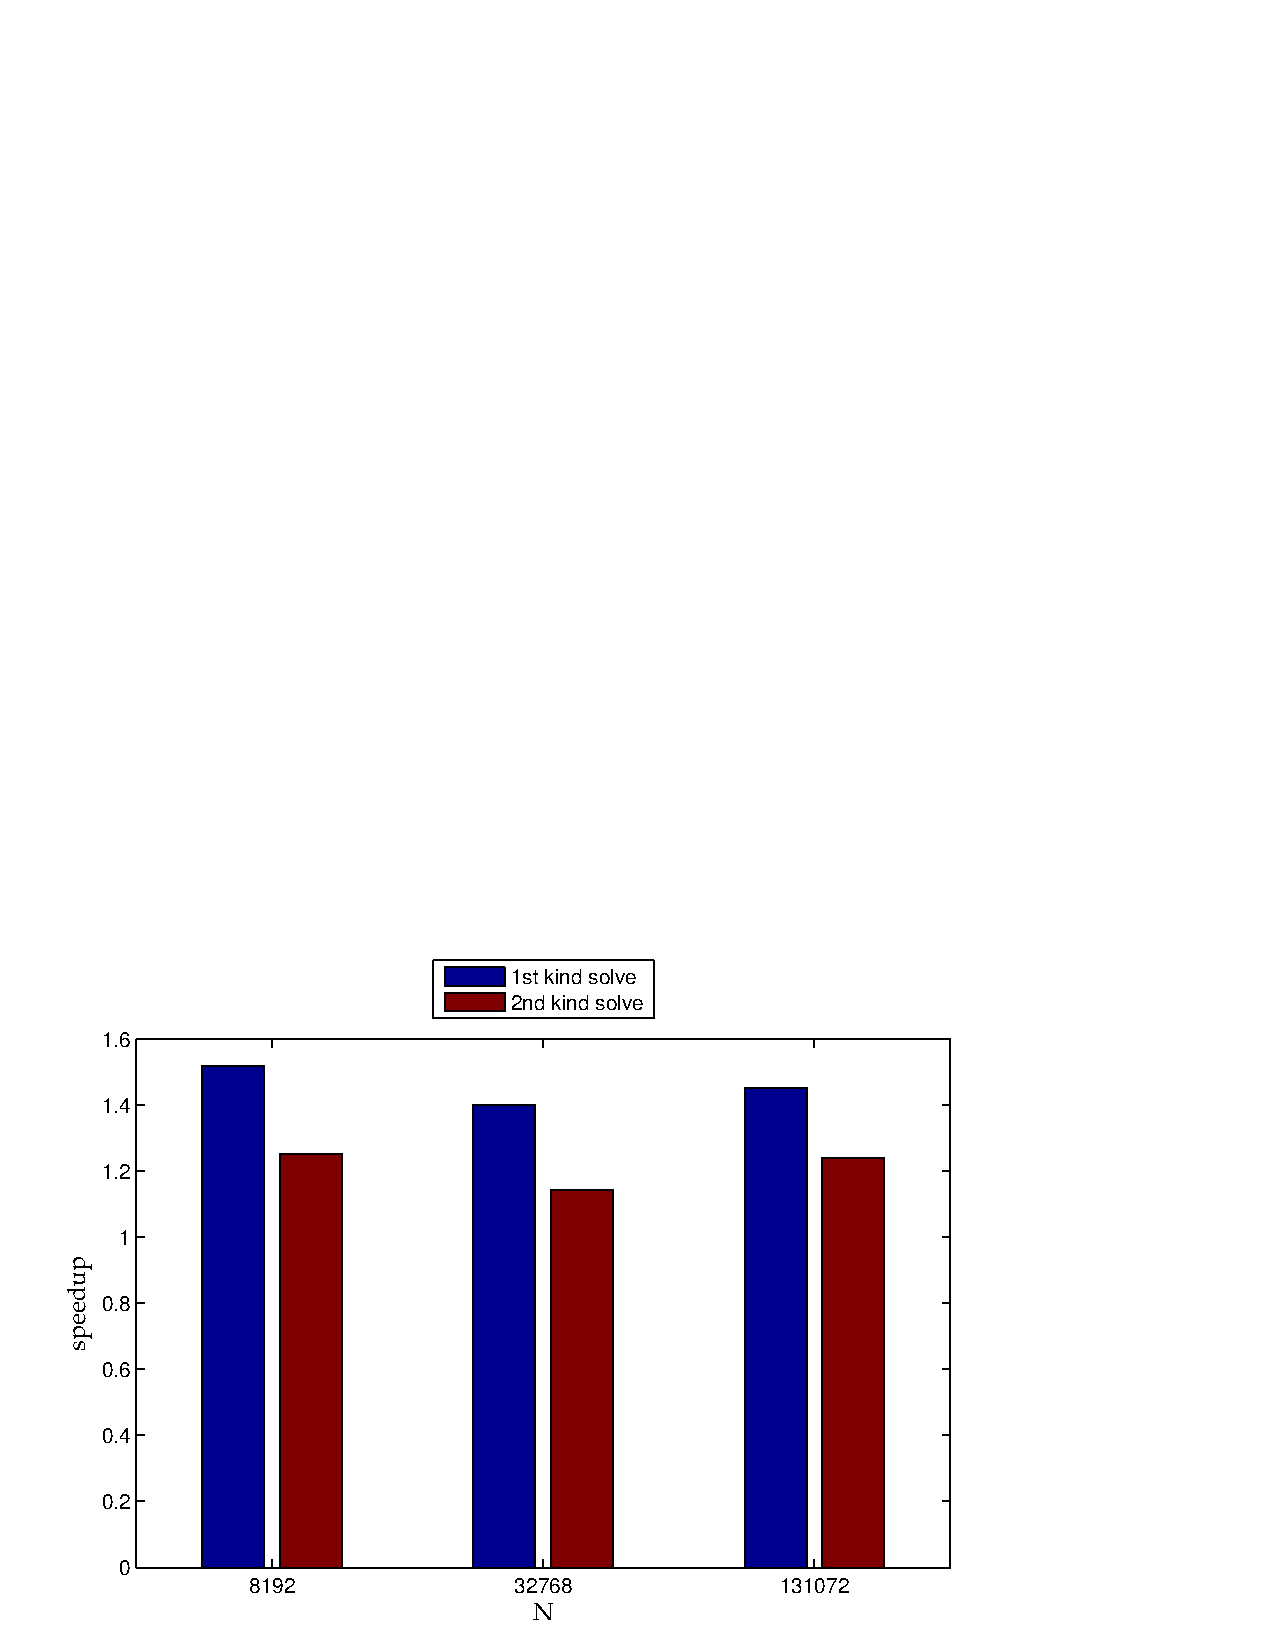
\includegraphics[width=14cm]{img/relaxation_timing_bar.pdf}
	\caption{Speedup using relaxation strategy}
	\label{fig:relaxation_timing}
\end{figure}

From tables \ref{tab:laplace_1st_relaxation} and \ref{tab:laplace_2nd_relaxation}, we can see that there is a benefit from using a relaxation scheme for these problems. For problem sizes of 8192 panels and above, we see an average speedup of around $1.4\times$ for 1st-kind solves and $1.2\times$ for 2nd-kind problems. While these are not huge speedups, they show the first successful application of a relaxation scheme to {\fmmbem}, as well as increasing speedups as problem sizes become larger.

Most interestingly, these results illustrate the differing parameters needed for optimal run times. The best choice of $\ncrit$ changes from $400$ in the non-relaxed case, to $200$ when a relaxed solver is used. This is logical, as for non-relaxed solves the best runtimes will be obtained by balancing the near and far-field evaluations ({\ptop} and {\mtol}). However, when we relax the system, the time taken for the far-field will decrease as a consequence of reducing $p$, while the amount of time for the {\ptop} will remain constant (as an aside, this could also be relaxed, but would necessitate creating a new tree every iteration). This means that to minimize time-to-solution for relaxed cases, we want to reduce this constant {\ptop} cost by adjusting $\ncrit$.

%From this figure, we can see the largest gains, as we might expect, from the larger problem sizes. For these problems, we have deeper trees, and thus more translation operators that will dominate with respect to $p$. This is likely to be the cause of the slightly decreasing speedup for 1st kind equations at the largest tested sizes, as the expensive first iterations dominate the total time taken. The most impressive (and increasing) speedups are for 2nd kind problems, which is encouraging as these constitute many engineering problems (Bioelectrostatics, acoustics).

Now that we have established that relaxation is successful in the sense that it a) converges to the correct answer, and b) provides a speedup in solve times over using a fixed $p$, we can investigate the kinds of situations that will provide the greatest benefits. To do this, we propose 2 hypotheses based on our initial results:

\begin{enumerate}
\item If a higher accuracy (and necessarily higher $p$) is needed, the benefits of relaxation will be greater, due to the ratio of work between the starting and minimum $p$ becoming greater. This hypothesis will be tested by solving a 1st-kind equation for 32768 panels, with varying values of starting $p$. To eliminate potential discrepancies in iteration count between values of $p$, and to recognize that not all problems are as simple to solve as the sphere, we enforce 10 {\gmres} iterations, resulting in a solve to $~5.5\times 10^{-5}$ tolerance. % This is equivalent to solving a slightly harder problem than the sphere, which is known to be comparatively easy. 

\item As more iterations are required, relaxed solves will spend more time at low values of $p$, and thus the speedups will be greater. We will test this hypothesis by artificially increasing the number of iterations in an analogous way to how we fixed the iteration count at 10 earlier. For this particular problem, increasing the number of iterations is equivalent to desiring a lower exit tolerance for the solver. 
\end{enumerate}

We now test both hypotheses, starting with the first; the relation between initial $p$ and overall speedup, using the sphere test case and forcing the solver to perform 10 iterations.

% N vs. p for converged answer
%   2048 : 5
%   8192 : 8
%  32768 : 10
% 131072 : 

% NOTE: at 32768 panels, behaviour is strange -- would need to work with higher k / solver tolerance

\begin{table}[h]
\begin{center}
\begin{tabular}{c|cc|cc|c}
  & \multicolumn{2}{c|}{Relaxed} & \multicolumn{2}{c|}{Non-Relaxed} & \\
  p & $\ncrit$ & $\tsolve$ & $\ncrit$ & $\tsolve$ & Speedup \\
   & & & & & \\ \hline
   & & & & & \\
  5 & 100 & 4.21 & 100 & 6.34 & 1.51 \\
   & & & & & \\
  8 & 100 & 6.24 & 400 & 12.4 & 1.99 \\
   & & & & & \\
  10 & 150 & 8.76 & 400 & 18.5 & 2.11 \\
   & & & & & \\
  12 & 150 & 13.2  & 600 & 25.3 & 1.92 \\
   & & & & & \\
  15 & 150 & 19.3 & 600 & 38.3 & 1.98 \\
 
\end{tabular}
\end{center}
\caption{Laplace 1st-kind relaxation speedup with respect to $p$ for sphere with 32768 panels.}
\label{tab:laplace_1st_p_relaxation}
\end{table}%

\begin{figure}[h]
	\centering
	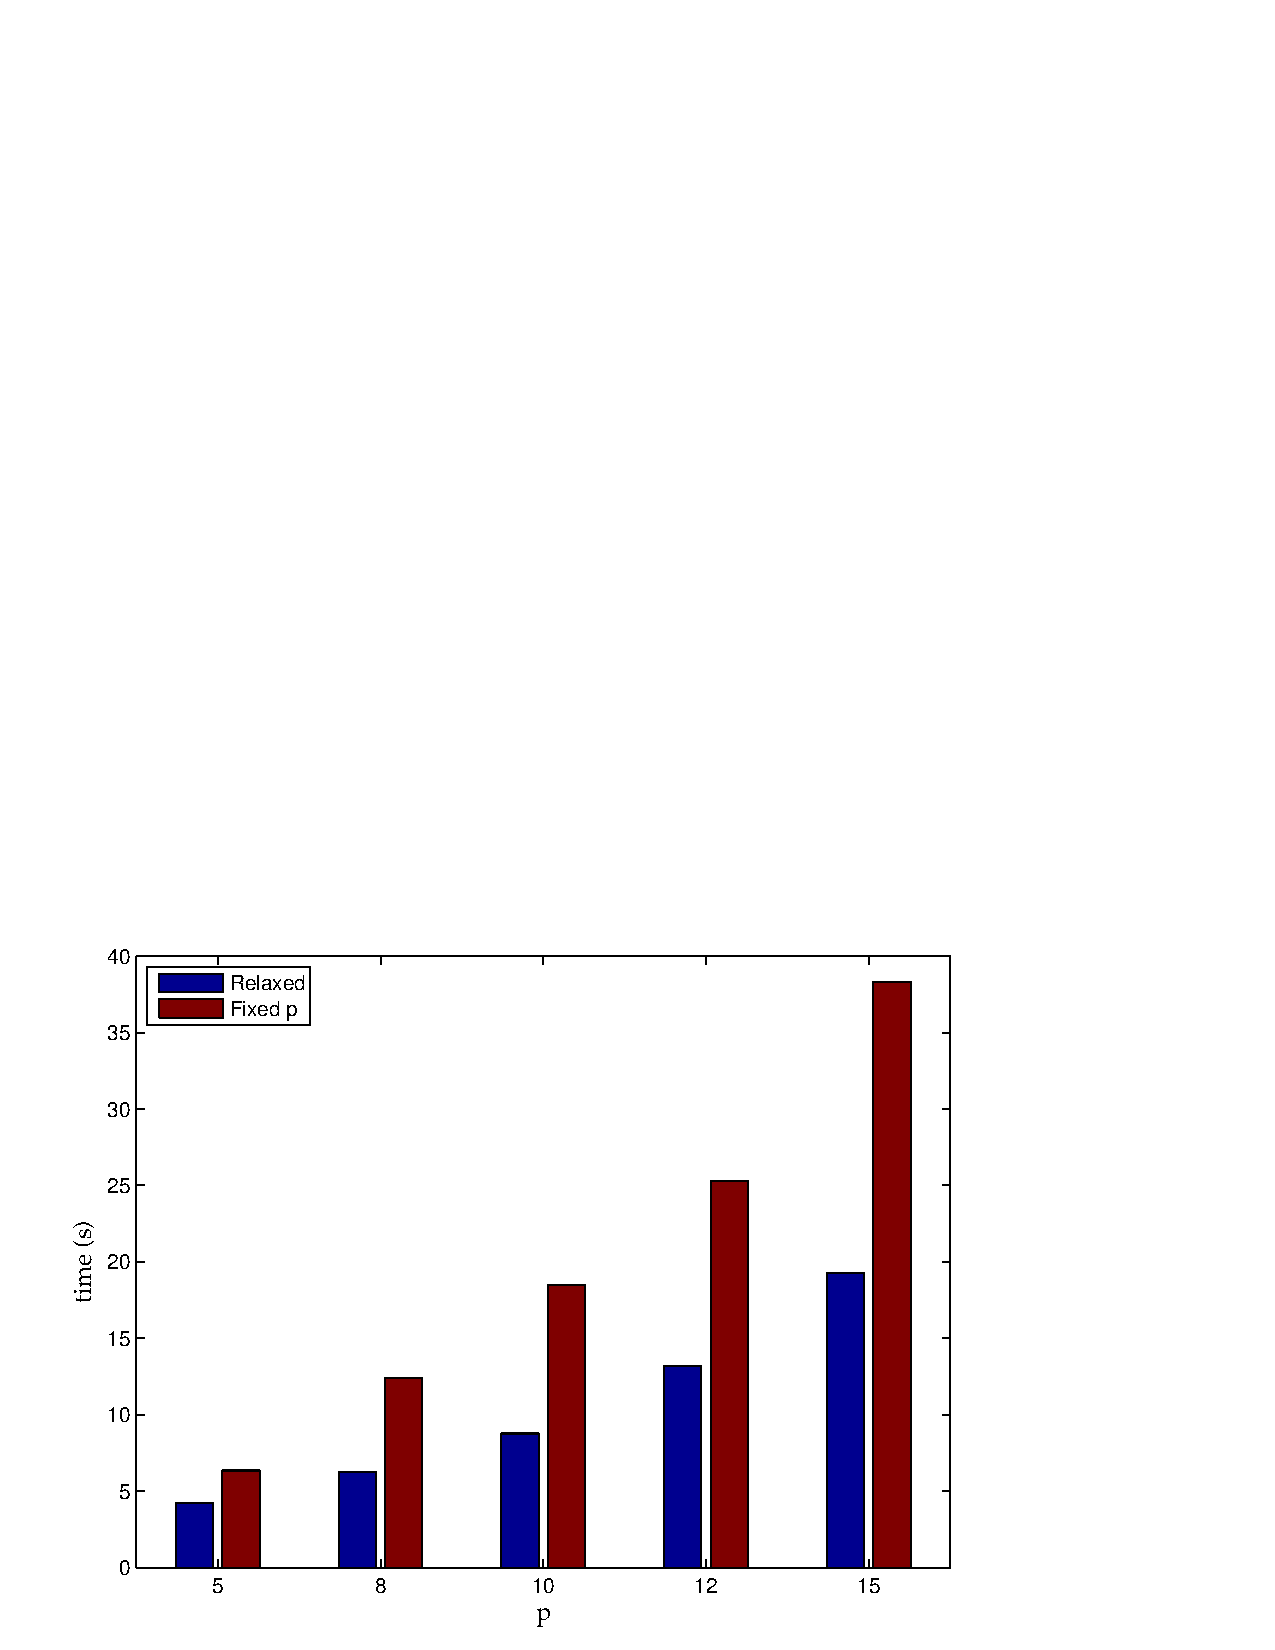
\includegraphics[width=14cm]{img/LaplaceRelaxationP.pdf}
	\caption{Time for 1st-kind Laplace equation solve on a sphere for 32768 panels with varying initial $p$ for relaxed and fixed-$p$ solvers. Iteration count capped at 10 for all cases.}
	\label{fig:laplace_p_speedup}
\end{figure}

The results in table \ref{tab:laplace_1st_p_relaxation} and summarized in figure \ref{fig:laplace_p_speedup} show a general trend -- at the lowest values of $p$ speedup is smaller, but it increases and levels out at approximately $2\times$ for larger tests. Looking at the times taken for individual iterations, this behaviour seems consistent. For the fastest total time, we desire an unbalanced tree on the first iteration (that is, where the time taken for near and far-fields is not equal), with the amount of {\ptop} kept artificially low.

While this means that later, low-$p$ iterations are very quick, it generally results in the first, high-$p$, iterations being slower than the equivalent fixed-$p$ case. Thus, the speedups obtained are purely from the low cost of the last iterations -- with higher $p$, the speedup in these iterations is greater, resulting in lower overall times to solution. The corollary of this, is that for lower initial $p$ the speedups from later iterations is smaller, thus the overall speedup is smaller.

%%% [[[ SPEEDUP TENDING TO NUMBER IF SIMILAR PATTERN OF REDUCING P? ]]]

To test the performance of relaxation with respect to higher iteration counts, we use the sphere problem again, artificially setting the desired number of {\gmres} iterations. This has the effect of progressively solving to lower tolerances, while eliminating potential discrepancies in iteration counts between the relaxed and fixed $p$ experiments. Table \ref{tab:laplace_1st_p_relaxation} shows these results. For all tests, the solver tolerance was disabled and initial $p = 10$. In all cases, a multi-threaded evaluator using 4 cores was used.

\begin{table}[H]
\begin{center}
\begin{tabular}{c|cc|cc|c}
  & \multicolumn{2}{c|}{Relaxed} & \multicolumn{2}{c|}{Non-Relaxed} & \\
  Iterations & $\ncrit$ & $\tsolve$ & $\ncrit$ & $\tsolve$ & Speedup \\
   & & & & & \\ \hline
   & & & & & \\
  5 & 100 & 8.57 & 400 & 10.0 & 1.17 \\
   & & & & &  \\
  10 & 100 & 9.81 & 400 & 18.4 & 1.88 \\
   & & & & & \\
  15 & 100 & 11.1 & 400 & 26.9 & 2.42 \\
   & & & & & \\
  20 & 100 & 12.4 & 400 & 35.3 & 2.85 \\
   & & & & & \\
  25 & 100 & 13.7 & 400 & 43.8 & 3.20 \\
   & & & & & \\
  50 & 100 & 20.6 & 400 & 86.2 & 4.18 \\
 
\end{tabular}
\end{center}
\caption{Laplace 1st-kind relaxation speedup with respect to iteration count for sphere with 32768 panels. $p=10$}
\label{tab:laplace_1st_iterations_relaxation}
\end{table}%

\begin{figure}[h]
	\centering
	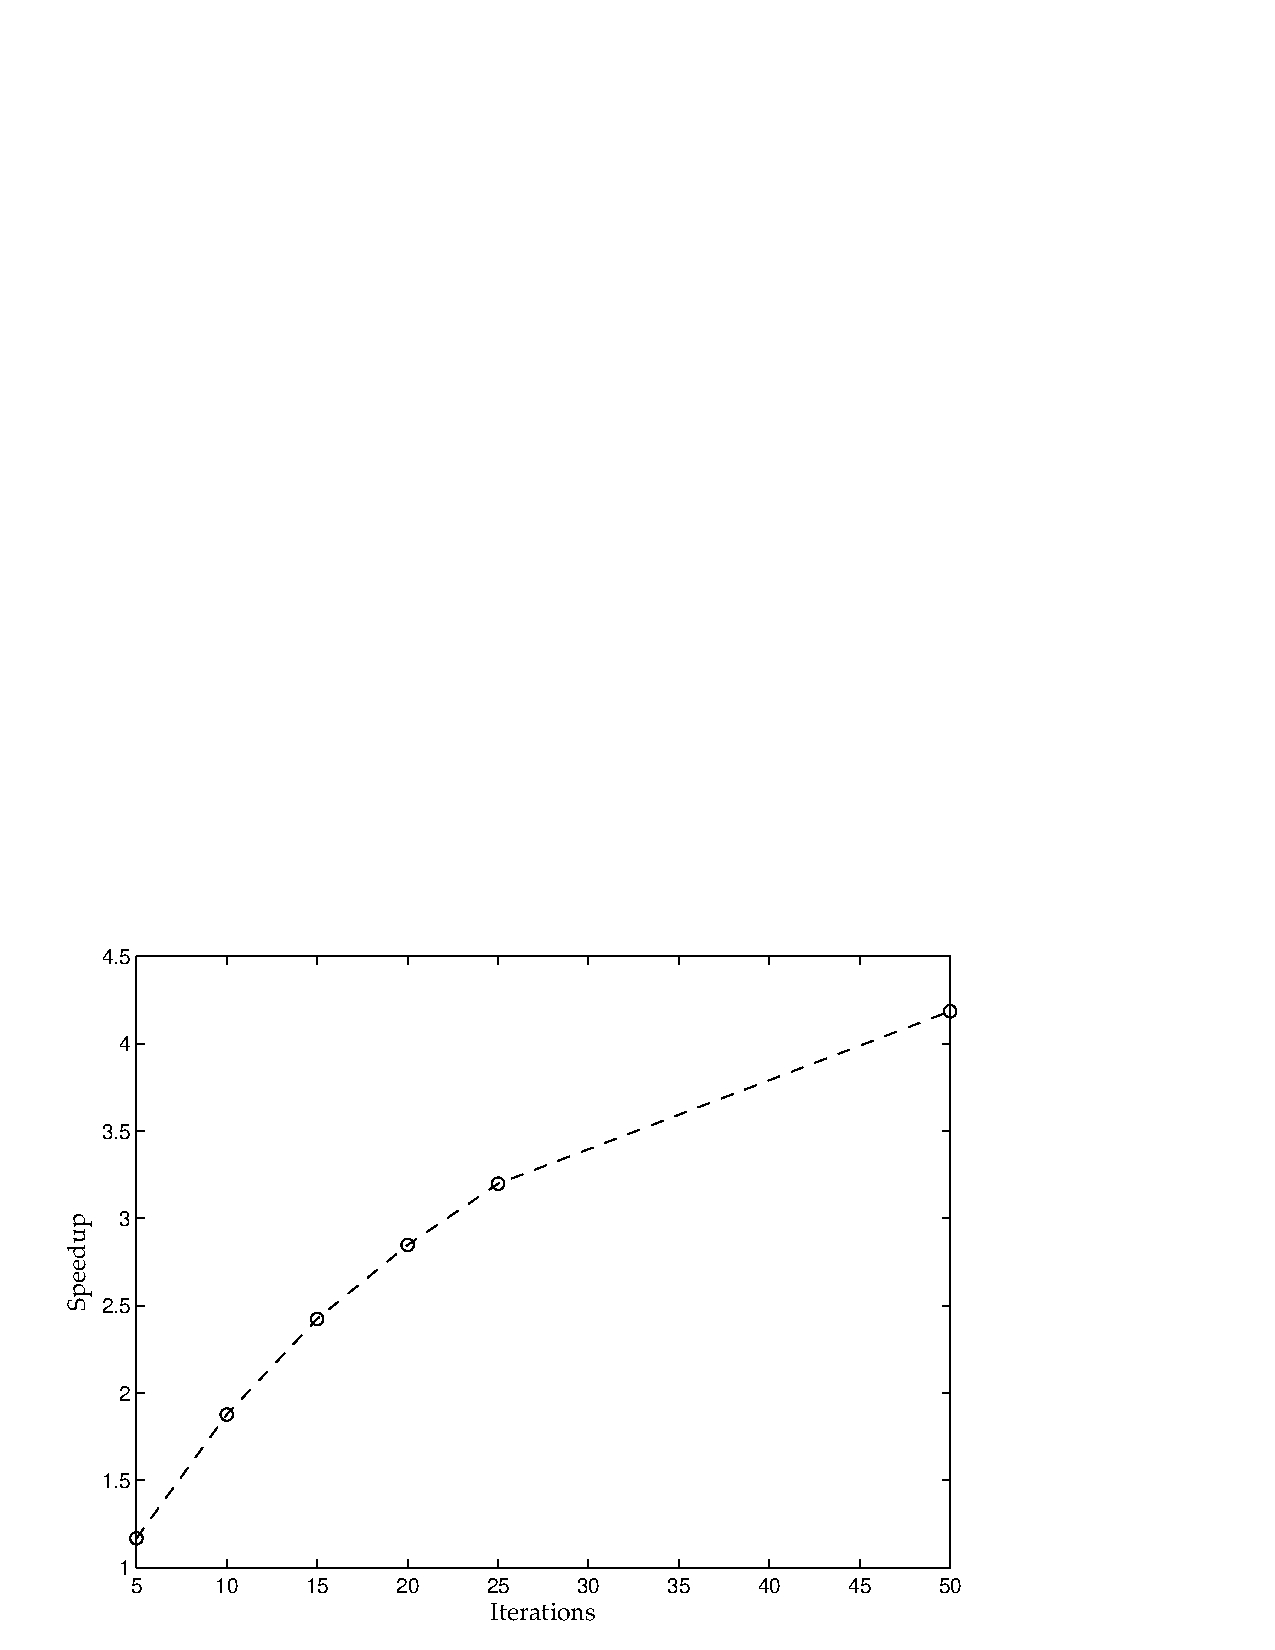
\includegraphics[width=14cm]{img/LaplaceRelaxationIterations.pdf}
	\caption{Speedup of 1st-kind Laplace solve on a sphere for 32768 panels with varying initial iteration count. $p=10$ for all cases.}
	\label{fig:laplace_iterations_speedup}
\end{figure}

From table \ref{tab:laplace_1st_iterations_relaxation} and figure \ref{fig:laplace_iterations_speedup}, the upward trend of speedup with respect to iteration count is very clear. From modest initial speedups, each increase in iterations gives a corresponding increase in acceleration. Further, we can see that each non-relaxed iteration adds approximately $1.68s$ to $\tsolve$, while each relaxed iteration adds a mere $0.276s$. Thus we can predict speedup as the iteration count continues to increase, with a $4.73\times$ acceleration predicted at 75 iterations, and $4.94\times$ at 100 iterations.

Combining our 2 earlier hypotheses and supporting results for both, we can now state that the optimal conditions for speedup from using a relaxation scheme are both a high iteration count, and high desired precision. Any problems exhibiting both these quantities should show significant speedups over standard solvers using a fixed $p$.

\section{Conclusions}\label{sec:laplace_conclusions}

In this section, we have laid the groundwork for applying relaxation schemes to {\fmmbem} problems. We have shown that our implementation is accurate, and that it converges as expected spatially. Beyond that, we have demonstrated the application of a relaxation scheme to {\fmmbem}, the first work of its kind. The parameter space for determining the expected speedup from relaxation has been explored, giving us confidence that any problems that require high accuracy and present tricky linear systems, resulting in many {\gmres} iterations, will give speedups in the order of $2-4\times$, a significant result.


\cleardoublepage

% -------------------------------------
% CHAPTER 6: STOKES
% -------------------------------------
%!TEX root = ../thesis.tex

\chapter{BEM with inexact GMRES for the Stokes equation}\label{chapter:stokes}
\thispagestyle{myheadings}

\graphicspath{{Stokes/}}

Now that we have demonstrated the ability of relaxed {\gmres} to correctly solve {\fmmbem} problems based on Laplace's equation and shown the speedups that this approach can give, we can continue to more substantial problems. Results from \S\ref{sec:laplace_relaxation} suggest that as $p$ increases the potential speedup from relaxation also increases. This implies that the benefits from relaxed solvers will increase with a corresponding need for accuracy. The next conclusion we can draw from the Laplace equation tests, is that we can correlate speedups with the number of iterations needed to solve -- in {\gmres} solvers, we spend a majority of iterations with residual values close to the desired final tolerance. As the linear system increases in difficulty to solve, we have more low-precision iterations and it is these iterations that will give us the greatest speedup.

The Stokes equation is a vector equation, and significantly more involved than Laplace, involving $62K$ operations for each $K$-th order integration between two panels, compared to $8K$ for Laplace. It is used in applications such as biomedicine \cite{RahimianETal2010} and MEMS (Microelectromechanical systems)\cite{fachinotti2007}. The use of {\fmmbem} for this equation is also well established \cite{Liu2009,gomez1997}. The difficulty of the resulting problems comes from both the added complications from the equation itself, requiring solving for 3 components (of velocity or surface traction) at every target panel, along with the more difficult linear systems that arise. Additional to these sources of complications, high precision is required in order to maintain accuracy \cite{Liu2009}. This combination of tough linear system, high accuracy and added difficulties within the integrals that must be computed, means we anticipate significant speedups from relaxing the solve, at least on par with those experienced in our Laplace experiments.

\section{Equation}

We start from the unsteady Navier-Stokes equations for fluid motion in terms of the velocity, $\vect{u}$, pressure, $p$, viscocity $\mu$ and fluid density $\rho$,
\begin{equation}
	\label{eqn:navier_stokes}
	\rho\left ( \partiald{\vect{u}}{t} + \vect{u}\cdot\nabla\vect{u}\right ) = -\nabla p + \mu\nabla^{2}\vect{u},
\end{equation}

\noindent
and concentrate on the case where the Reynolds number, $Re_L = \rho UL / \mu$ is small, or in other words,  diffusion effects $\nabla^{2}\vect{u}$ are much larger than convective effects, $\vect{u}\cdot\nabla\vect{u}$.
\begin{equation}
	\nabla^{2}\vect{u} \gg \vect{u}\cdot\nabla\vect{u}
\end{equation}

In this case, we obtain 2 equations, the Stokes equation \eqref{eqn:stokes} and the linearized Navier-Stokes equation \ref{eqn:linearized_ns} for the steady and unsteady cases respectively.
\begin{eqnarray}
	\label{eqn:stokes}\mu\nabla^{2}\vect{u} & = & \nabla p \\
	\label{eqn:linearized_ns}\rho\partiald{\vect{u}}{t} & = & -\nabla p + \mu\nabla^{2}\vect{u}.
\end{eqnarray}

Similar to the Laplace equation, we want the fundamental solution(s) for equation \ref{eqn:stokes}, and these are the Stokeslet \ref{eqn:stokeslet} and the stresslet \ref{eqn:stresslet}, shown in both matrix and tensor notation forms.

%We find that the fundamental solutions to \ref{eqn:stokes} are the stokeslet \ref{eqn:stokeslet}, [[[MORE HERE]]] \ref{eqn:stokeslet_2} 

\begin{eqnarray}
	\label{eqn:stokeslet}
	S_{ij}(\vect{x},\vect{y}) & = & \frac{\delta_{ij}}{r} + \frac{(x_i-y_i)(x_j-y_j)}{r^{3}} \\
	& & \nonumber \\
	\label{eqn:stokeslet_2}
		   & = & \frac{1}{r^{3}}\left (
	\begin{array}{ccc}
		r^{2} + dx^{2} & dx\cdot dy & dx\cdot dz \\
		dx\cdot dy & r^{2} + dy^{2} & dy\cdot dz \\
		dx\cdot dz & dy\cdot dz & r^{2} + dz^{2}
	\end{array} \right )
\end{eqnarray}

%\noindent	
%and the stresslet \ref{eqn:stresslet}, \ref{eqn:stresslet_2}

\begin{eqnarray}
	\label{eqn:stresslet}
	%D_{ij}(\vect{x},\vect{y},\vect{\hat{n}}) & = & \frac{1}{6}\sum_{k=1}^{3}\left [ \left( \delta_{ij} - (x_j-y_j)\partiald{}{x_i}\right ) \frac{(x_k-y_k)\hat{n}_k}{r^{3}} \right . \nonumber \\ 
%& & + \left . \left (\delta_{ik}-(x_k-y_k)\partiald{}{x_i}\right )\frac{(x_j-y_j)\hat{n}_k}{r^{3}}\right ] \\
	T_{ijk}(\vect{x},\vect{y},\nhat) & = & 6\frac{(x_i-y_i)(x_j-y_j)(x_k-y_k)n_k}{r^{5}} \\
	& & \nonumber \\ 
	\label{eqn:stresslet_2}
	& = & 6\frac{(\di{\vect{x}}\cdot\vect{\hat{n}})}{r^{5}}\left (\begin{array}{ccc}
		dx^{2} & dx\cdot dy & dx\cdot dz \\
		dx\cdot dy & dy^{2} & dy\cdot dz \\
		dx\cdot dz & dy\cdot dz & dz^{2}
	\end{array} \right )
\end{eqnarray}

These fundamental solutions will be used in the next section when we formulate a {\bem} form of the Stokes equation, suitable for solving with the framework used throughout this thesis.  
		
\section{BEM}

Similar to how we began from Green's second identity while deriving the boundary integral form of the Laplace equation, we start here from Lorentz's reciprocal relation, similar to standard derivations \cite{Pozrikidis1992,Liu2009}.

\begin{eqnarray}
	\label{eqn:stokes_bem_1}\nabla\cdot\left ( \vect{u}'\cdot\vect{\sigma} - \vect{u}\cdot\vect{\sigma}'\right ) & = & 0 \\
	\label{eqn:stokes_bem_2}\partiald{}{x_k}\left ( u_i'\sigma_{ik} - u_i\sigma_{ik}' \right ) & = & 0,
\end{eqnarray}

\noindent
where $\vect{u}$ and $\vect{u}'$ are solutions to Stokes equations, and $\vect{\sigma}$ and $\vect{\sigma}'$ are the associated stress tensors. Looking at the domain in figure \ref{fig:stokes_volume}, if we identify $\vect{u}'$ as the velocity induced from a point source with strength $\vect{g}$, we can obtain

\begin{figure}[h]
\begin{center}
	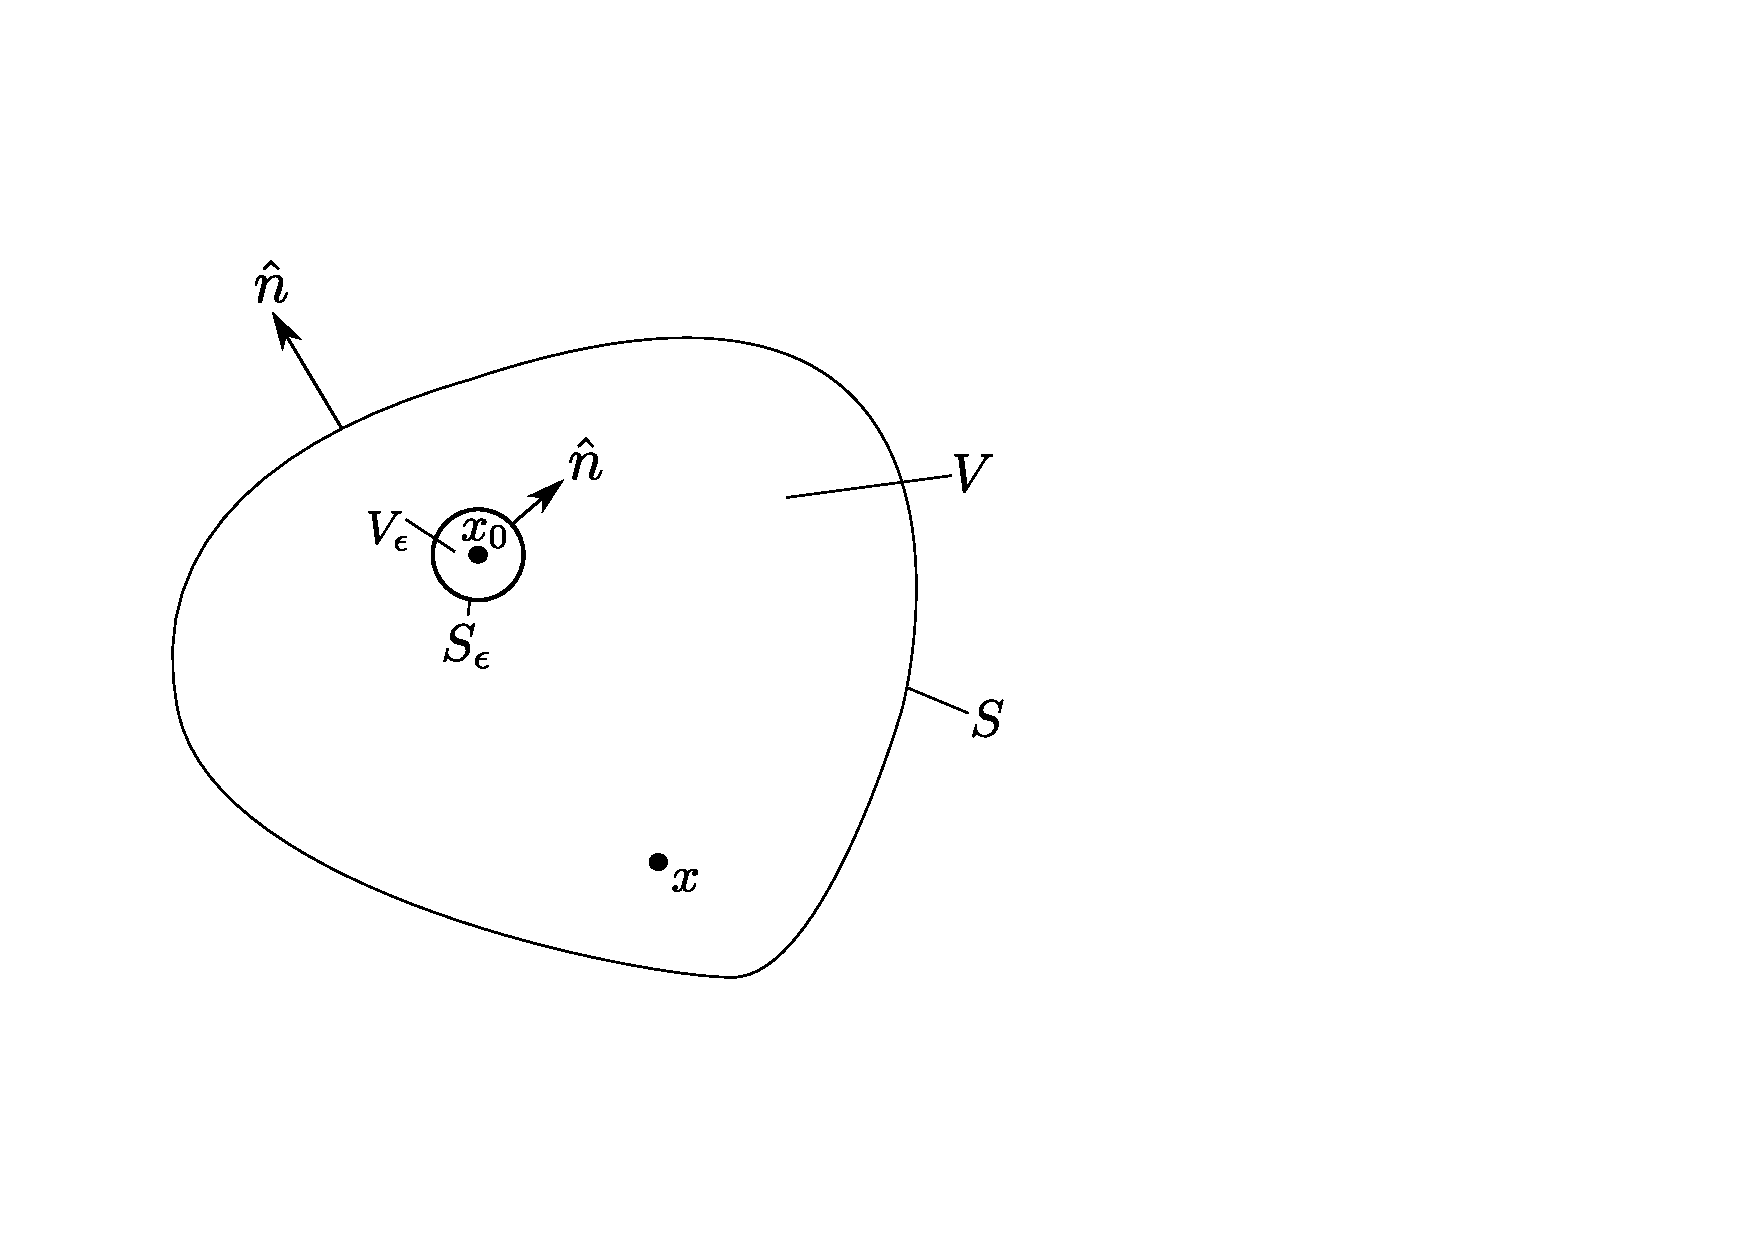
\includegraphics[width=12cm]{img/StokesVolume.pdf}
	\caption{Domain used for derivation of Stokes boundary integral equation}
	\label{fig:stokes_volume}
\end{center}
\end{figure}

\begin{equation}
	\label{eqn:stokes_bem_3} u_i(\vect{x}) = \frac{1}{8\pi\mu}G_{ij}(\vect{x},\vect{x}_0)g_j,\;\;\;\;\sigma_{ijk}' = \frac{1}{8\pi}T_{ij}(\vect{x},\vect{x}_0,\nhat)g_j.
\end{equation}

Discarding $\vect{g}$ as a constant, and substituting \ref{eqn:stokes_bem_3} into \ref{eqn:stokes_bem_2}, we get

\begin{equation}
	\label{eqn:stokes_bem_4}
	\partiald{}{x_k}\left ( G_{ij}(\vect{x},\vect{x}_0)\sigma_{ik}(\vect{x}) - \mu u_i(\vect{x})T_{ijk}(\vect{x},\vect{x}_0)\right ) = 0.
\end{equation}

Next, we integrate \ref{eqn:stokes_bem_4} over a volume, $V$, set $\vect{x}_0$ outside of $V$ and apply the divergence theorem

\begin{equation}
	\label{eqn:stokes_bem_5}
	\int_{\Gamma} \left [ G_{ij}(\vect{x},\vect{x}_0)\sigma_{ik}(\vect{x}) -\mu u_i(\vect{x})T_{ijk}(\vect{x},\vect{x}_0)\right ]\hat{n}_k(\vect{x})\di{\vect{S}}(\vect{x}) = 0.
\end{equation}

Next, moving $\vect{x}_0$ towards the surface, we select $V_\epsilon$ as a small spherical volume around $\vect{x}_0$ with radius $\epsilon$. Integrating over $V-V_\epsilon$ and using the divergence theorem once more

\begin{equation}
	\label{eqn:stokes_bem_6}
	\int_{\Gamma,S_\epsilon} \left [ G_ij(\vect{x},\vect{x}_0)\sigma_{ik}(\vect{x}) -\mu u_i(\vect{x})T_{ijk}(\vect{x},\vect{x}_0)\right ]\hat{n}_k(\vect{x})\di{\vect{S}}(\vect{x}) = 0.
\end{equation}

Letting $\epsilon\to 0$, $\vect{G}, \vect{T}$ reduce to the Stokeslet and stresslet,

\begin{equation}
	\label{eqn:stokes_bem_7}
	G_{ij} = S_{ij} = \frac{\delta_{ij}}{\epsilon} + \frac{\hat{x}_i\hat{x}_j}{\epsilon^{3}}, \;\;\;\; T_{ijk} = -6\frac{\hat{x}_i\hat{x}_j\hat{x}_k}{\epsilon^{5}},
\end{equation}

\noindent
with $\hat{x}_i = x_i - x_{0i}$. Over the volume $S_\epsilon$, $\hat{n} = \hat{x}/\epsilon$ and $\di{\vect{S}} = \epsilon^{2}\di{\Omega}$. Substituting \ref{eqn:stokes_bem_7} into \ref{eqn:stokes_bem_6} we now obtain
\begin{equation}
	\label{eqn:stokes_bem_8}
	\begin{multlined}
	\int_{\Gamma,S_\epsilon} \left [ G_ij(\vect{x},\vect{x}_0)\sigma_{ik}(\vect{x}) -\mu u_i(\vect{x})T_{ijk}(\vect{x},\vect{x}_0)\right ]\hat{n}_k(\vect{x})\di{\vect{S}}(\vect{x}) = \\
	-\int_{S_\epsilon} \left [ \left ( \delta_{ij} + \frac{\hat{x}_i\hat{x}_j}{\epsilon^{2}} \right )\sigma_{ik}(\vect{x}) + 6\mu u_i(\vect{x})\frac{\hat{x}_i\hat{x}_j\hat{x}_k}{\epsilon^{4}} \right ]\hat{x}_k\;\di{\Gamma}.
	\end{multlined}
\end{equation}

When we take the limit $\epsilon\to 0$, $\vect{u}$ and $\vect{\sigma}$ over the volume $S_\epsilon$ tend to $\vect{u}(\vect{x}_0)$ and $\vect{\sigma}(\vect{x}_0)$. We also note that as $\epsilon\to 0$ the stress term on the right-hand-side of \ref{eqn:stokes_bem_8} will decrease linearly, while the velocity term will tend to a constant,

\begin{equation}
	\label{eqn:stokes_bem_9}
	-6\mu u_i(\vect{x}_0)\frac{1}{\epsilon^{4}}\int_{S_\epsilon} \hat{x}_i\hat{x}_j\;\di{S(\vect{x})}.
\end{equation}

Applying the divergence theorem to the surface integral in \ref{eqn:stokes_bem_9}, we get

\begin{equation}
	\label{eqn:stokes_bem_10}
	\int_{S_\epsilon} \hat{x}_i\hat{x}_j\;\di{S(\vect{x})} = \epsilon\int_{S_\epsilon}\hat{x}_i\hat{n}_j\;\di{S(\vect{x})} = \epsilon\int_{V_\epsilon}\partiald{\hat{x}_i}{\hat{x}_j}\;\di{V(\vect{x})} = \delta_{ij}\frac{4}{3}\pi\epsilon^{4}.
\end{equation}

Finally plugging \ref{eqn:stokes_bem_10} into \ref{eqn:stokes_bem_8} (with the right hand side collapsed to \ref{eqn:stokes_bem_9}), we get the expected boundary integral form:

\begin{equation}
	\label{eqn:stokes_bem_11}
	u_j(\vect{x_0}) = -\frac{1}{8\pi\mu}\int_{\Gamma} \sigma_{ik}(\vect{x})n_k(\vect{x})G_{ij}(\vect{x},\vect{x}_0)\;\di{S(\vect{x})} + \frac{1}{8\pi} \int_{\Gamma} u_i(\vect{x})T_{ijk}(\vect{x},\vect{x}_0)n_k(\vect{x})\;\di{S(\vect{x})}.
\end{equation}

Setting $t = \sigma\cdot\nhat$ and taking $\vect{x}_0$ to a smooth part of the boundary, \\
$\int_{\Gamma} u_i(\vect{x})T_{ijk}(\vect{x},\vect{x}_0)n_k(\vect{x})\;\di{\Gamma(\vect{x})} \to 0$, and $\int_{\Gamma} \sigma_{ik}(\vect{x})n_k(\vect{x})G_{ij}(\vect{x},\vect{x}_0)\;\di{\Gamma(\vect{x})} \to 1/2$. This gives the final form of the boundary integral equation before discretization

%Taking $\vect{x}_0$ to the boundary, and setting $t = \sigma\nhat$, we introduce a constant, $c_{ij}$ in front of the initial $u_j$, and when we take $\vect{x}_0$ to the centre of a smooth surface (such as in collocation) $c_{ij} = \delta_{ij}\frac{1}{2}$. Applying this to \ref{eqn:stokes_bem_11} along with denoting the surface traction force, $\vect{t}(\vect{x}) = \sigma_{ik}(\vect{x})n_k(\vect{x})$, we obtain the final, implemented form of the boundary integral equation

\begin{equation}
	\label{eqn:stokes_bem_12}
	\frac{1}{2}u(\vect{x_0}) = -\frac{1}{8\pi\mu}\int_{\Gamma} t_i(\vect{x})G_{ij}(\vect{x},\vect{x}_0)\;\di{\Gamma} + \frac{1}{8\pi} \int_{\Gamma} u_i(\vect{x})T_{ijk}(\vect{x},\vect{x}_0)n_k(\vect{x})\;\di{\Gamma}.
\end{equation}

Finally discretizing with constant panels we obtain

\begin{equation}
	\label{eqn:stokes_bem_discretized}
	\frac{1}{2}u_i(\vect{x_0}) = -\frac{1}{8\pi\mu}\sum_{j=1}^{N}t_j\int_{\Gamma} G_{ij}\;\di{\Gamma_j} + \frac{1}{8\pi} \sum_{j=0}^{N}u_j\int_{\Gamma} T_{ijk}\cdot n_k\;\di{\Gamma_j}.
\end{equation}

\section{Expansions}\label{sec:stokes_expansions}

To approximate the Stokeslet and stresslet we use a method based on decomposing \ref{eqn:stokeslet} and \ref{eqn:stresslet} into sets of harmonic equations, each suitable to be approximated using the Laplace FMM from \S\ref{sec:laplace_expansions} and recombined to give the full answer \cite{tornberg2008}.

First, we can write the Stokeslet $S_{ij}$ as
\begin{equation}
	S_{ij} = \left ( \delta_{ij} - (x_j-y_j)\partiald{}{x_i}\right)\frac{1}{|\vect{x}_i-\vect{x}_j|},
\end{equation}

\noindent
and $F_i^{m} = F_i(\vect{x}_m)$ as
\begin{equation}
	F_i^{m} = \sum_{n=0}^{N} S_{ij}(\vect{x}_m,\vect{x}_n)\cdot \vect{f}_n
\end{equation}

Then, we can perform more manipulations to get another alternate form,

\begin{equation}
	F_i^{m} = \sum_{j=1}^{3}\left [ \left (\delta_{ij}-x_j^{m}\partiald{}{x_i}\right) \sum_{n=1}^{N}\frac{f^{n}_j}{r_{nm}} \right ] + \partiald{}{x_i}\sum_{n=1}^{N}\frac{\vect{x}^{n}\cdot \vect{f}^{n}}{r_{nm}}.
\end{equation}

This decomposition lets us approximate the Green's function operator with 4 Laplace {\fmm}s for $1/r$, with  source strengths $f^{n}_1,\;f^{n}_2,\;f^{n}_3,\;(\vect{x}^{n}\cdot\vect{f}^{n})$. Similarly, we can rewrite the stresslet, $D_{ij}$ in a similar form:

\begin{equation}
	\begin{multlined}
	D_{ij}(\vect{x},\vect{y},\nhat) = \frac{1}{6}\sum_{k=1}^{3} \left [ \left ( \delta_{ij} - (x_j-y_j)\partiald{}{x_i} \right )\frac{(x_k-y_k)\nhat_k}{|\vect{x}-\vect{y}|^{3}} \right . \\
	+ \left . \left ( \delta_{ik}-(x_k-y_k)\partiald{}{x_i}\right )\frac{(x_j-y_j)\nhat_k}{|\vect{x}-\vect{y}|^{3}} \right ]
	\end{multlined}
\end{equation}

\noindent
and $G_i^{m} = G_i(\vect{x}_m)$ as

\begin{equation}
	G_i^{m} = \sum_{n=0}^{N} D(\vect{x}_m,\vect{x}_n,\nhat_n)\cdot\vect{g}_n
\end{equation}

\begin{equation}
	\begin{multlined}
	G_i^{m} = \frac{1}{6}\sum_{j=1}^{3} \left [ \left ( \delta_{ij}-x_j^{m}\partiald{}{x_i}\right ) \sum_{n=1}^{N} \left \{ \frac{(\vect{r}_{nm}\cdot\vect{\nhat}^{n})g^{n}_{j}}{r_{nm}^{3}} + \frac{(\vect{r}_{nm}\cdot\vect{g}^{n})\nhat^{n}_{j}}{r_{nm}^{3}} \right \} \right ] \\
	+ \frac{1}{6}\partiald{}{x_i}\sum_{n=1}^{N} \left \{ \frac{(\vect{r}_{nm}\cdot\vect{\nhat}^{n})(\vect{x}^{n}\cdot\vect{g}^{n})}{r_{nm}^{3}} + \frac{ (\vect{r}_{nm}\cdot\vect{g}^{n})(\vect{\nhat}^{n}\cdot\vect{x}^{n})}{r_{nm}^{3}} \right \}
	\end{multlined}
\end{equation}

Similar to the Stokeslet case, we are able to approximate the Stresslet using 4 harmonic approximations, this time for $1/r^{3}$, where every particle contributes 2 dipoles to each approximation. 

\begin{eqnarray}
	& &(\vect{r}_{nm}\cdot\vect{\nhat}^{n})g^{n}_{1} + (\vect{r}_{nm}\cdot\vect{g}^{n})\nhat^{n}_{1} \\
	& &(\vect{r}_{nm}\cdot\vect{\nhat}^{n})g^{n}_{2} + (\vect{r}_{nm}\cdot\vect{g}^{n})\nhat^{n}_{2} \\
	& &(\vect{r}_{nm}\cdot\vect{\nhat}^{n})g^{n}_{3} + (\vect{r}_{nm}\cdot\vect{g}^{n})\nhat^{n}_{3} \\
	& &(\vect{r}_{nm}\cdot\vect{\nhat}^{n})(\vect{x}^{n}\cdot\vect{g}^{n}) + (\vect{r}_{nm}\cdot\vect{g}^{n})(\vect{\nhat}^{n}\cdot\vect{x}^{n})
\end{eqnarray}�
%
%\begin{eqnarray}
%	M_1 & = & \sum_{n=1}^{N} \left \{\frac{(\vect{r}_{nm}\cdot\vect{\nhat}^{n})g^{n}_{1}}{r_{nm}^{3}} + \frac{(\vect{r}_{nm}\cdot\vect{g}^{n})\nhat^{n}_{1}}{r_{nm}^{3}} \right \}\\
%	M_2 & = & \sum_{n=1}^{N}\left\{\frac{(\vect{r}_{nm}\cdot\vect{\nhat}^{n})g^{n}_{2}}{r_{nm}^{3}} + \frac{(\vect{r}_{nm}\cdot\vect{g}^{n})\nhat^{n}_{2}}{r_{nm}^{3}}\right\} \\
%	M_3 & = & \sum_{n=1}^{N}\left\{\frac{(\vect{r}_{nm}\cdot\vect{\nhat}^{n})g^{n}_{3}}{r_{nm}^{3}} + \frac{(\vect{r}_{nm}\cdot\vect{g}^{n})\nhat^{n}_{3}}{r_{nm}^{3}}\right\} \\
%	M_4 & = & \sum_{n=1}^{N}\left\{\frac{(\vect{r}_{nm}\cdot\vect{\nhat}^{n})(\vect{x}^{n}\cdot\vect{g}^{n})}{r_{nm}^{3}} + \frac{ (\vect{r}_{nm}\cdot\vect{g}^{n})(\vect{\nhat}^{n}\cdot\vect{x}^{n})}{r_{nm}^{3}}\right\}
%\end{eqnarray}

When we come to evaluate all of these expansions, we note that both the Stokeslet and stresslet are of the same form, just with different source strengths for each expansions. Assuming our 4 expansions $M_i,\;i=1..4$ are ordered in the same way we defined the influences of particles earlier,

\begin{equation}
	\phi^{m}_i = \sum_{j=1}^{3} \left ( \delta_{ij} - x_j^{m}\partiald{}{x_i}\right ) M_j + \partiald{}{x_i}M_4.
\end{equation}

\section{Convergence}\label{sec:stokes_convergence}

Just as for the Laplace equation, we wish to show our method is working as intended, and thus converges to the correct accuracy as a function of the spatial discretization. For the Stokes equations, we choose to simulate the low-Reynolds number flow over a sphere. A classical problem in Stokes flow, when placed in a uniform flow of speed $u_x$, the drag over the sphere can be found analytically to be $F_d = 6\pi\mu Ru_x$.

Imposing $\vect{u} = (1,0,0)^{T}$ at the center of every panel, we solve a first-kind equation for the traction force, $\vect{t}$, from which we can then get the total drag force from the integral

\begin{equation}
	\label{eqn:stokes_traction_drag}
	F_d = \int_\Gamma t_x\;\di{\Gamma'} = \sum_{j=1}^{N} t_{x_j}\cdot A_j
\end{equation}

In these tests, we set $R=1$, $u_x = 1$ and $\mu = 10^{-3}$, giving a drag force of $F_d = 0.01885$. For each case, $p$ was increased until the solution stopped improving. Figure \ref{fig:stokes_sphere_traction} shows the $t_x$, the traction force exerted in the $x$-direction on the sphere

\begin{figure}[h]
\begin{center}
	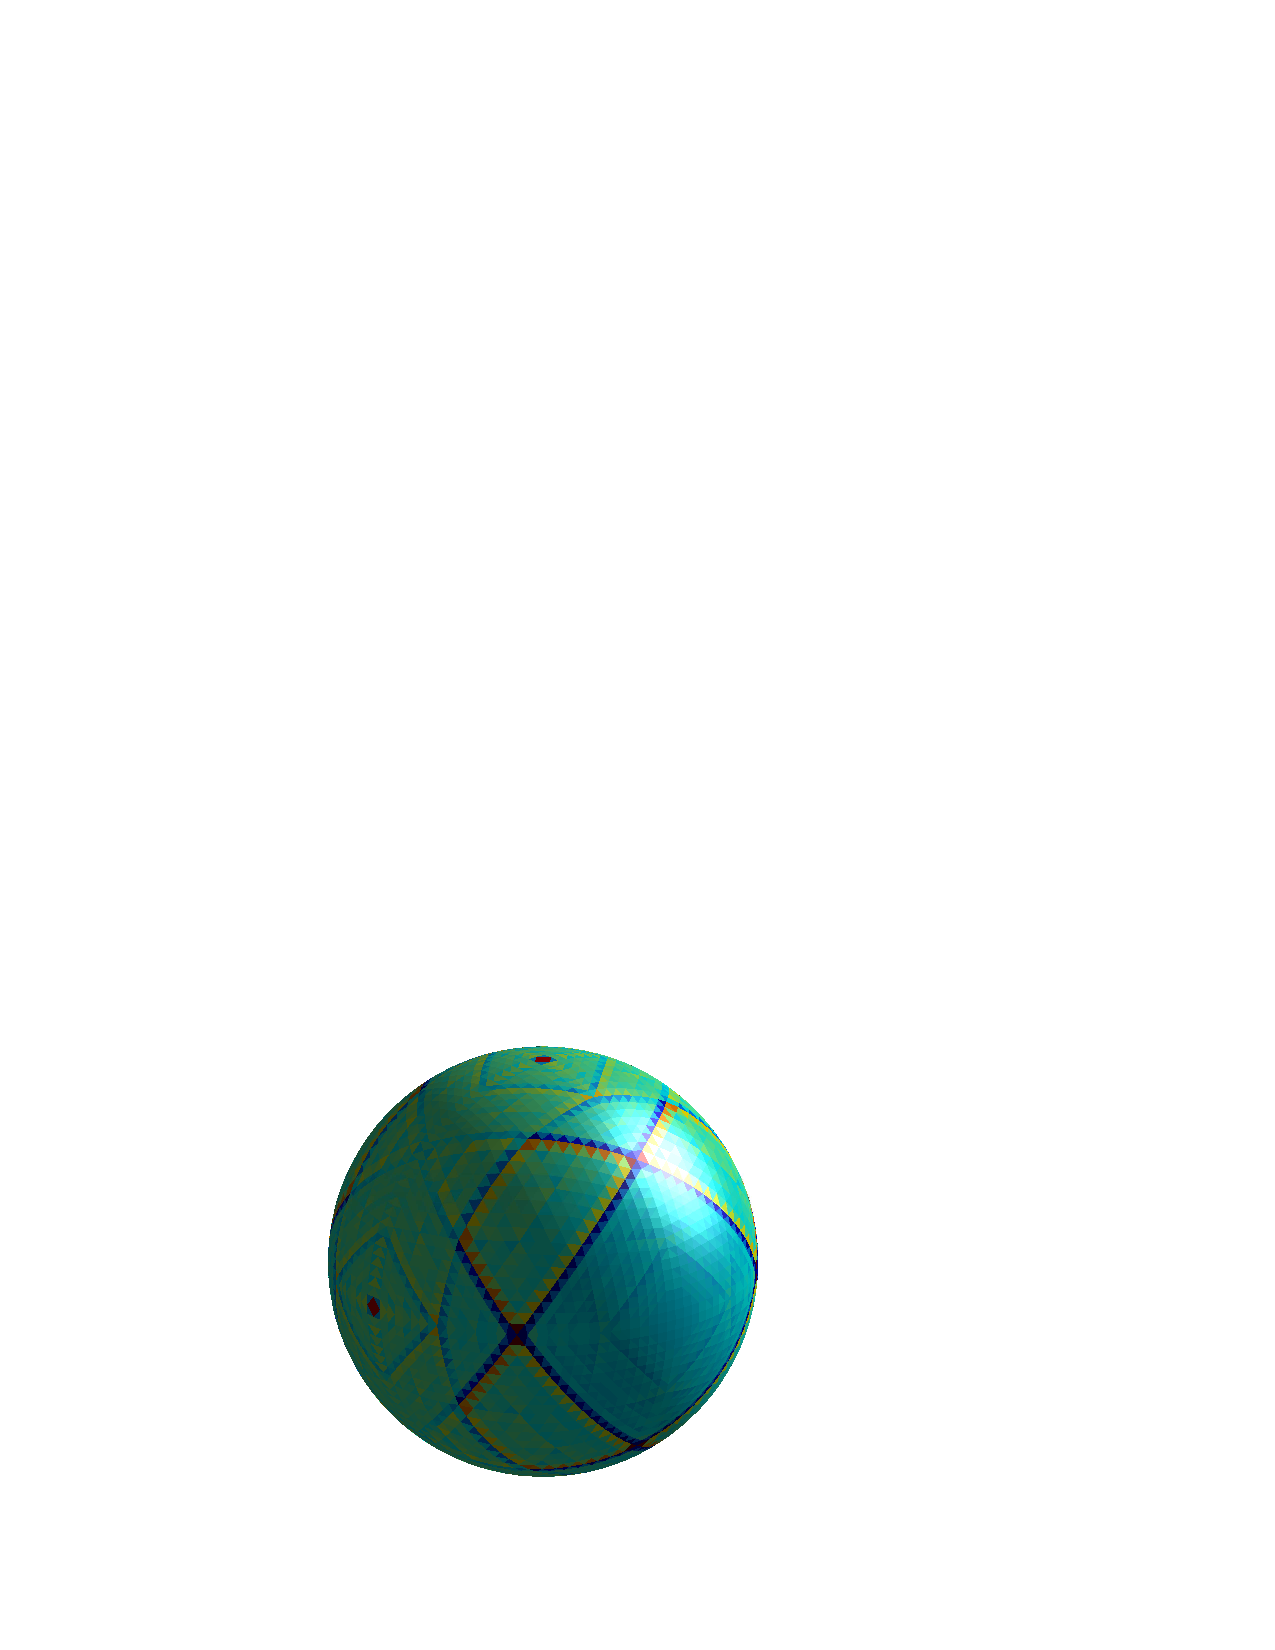
\includegraphics[width=12cm]{img/StokesTraction2.pdf}
	\caption{Traction force $t_x$ exerted in the $x$-direction on a sphere, 32768 panels, $p=16$, $\pmin=5$ solved to $10^{-5}$ tolerance.}
	\label{fig:stokes_sphere_traction}
\end{center}
\end{figure}

It is worth pointing out that while we do have some oscillations in the traction force, their magnitude is small ($\O{10^{-4}}$), and they do not affect the derived quantity (in this case, total drag force) that we are interested in.

\begin{figure}[h]
\begin{center}
	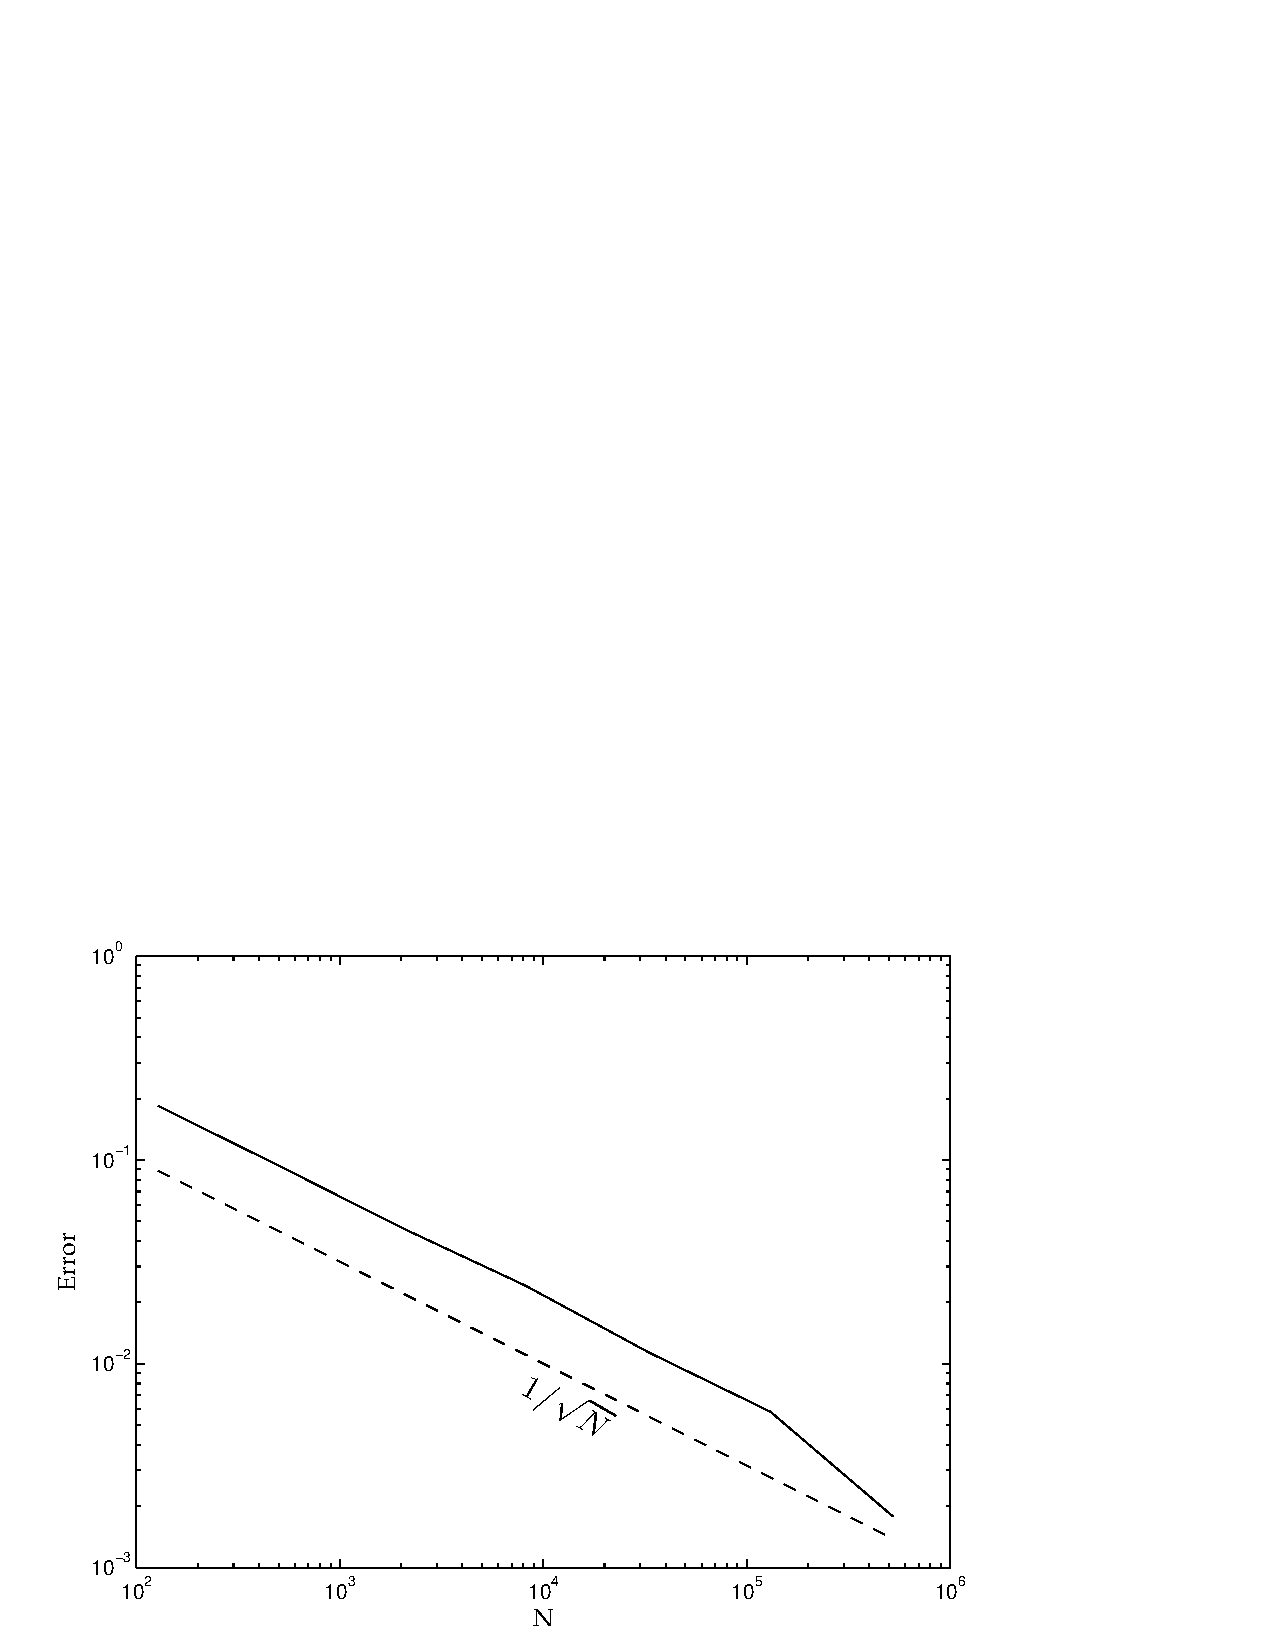
\includegraphics[width=14cm]{img/StokesConvergence.pdf}
	\caption{Convergence of first-kind equation for Stokes flow around a sphere. Initial $p=16$, linear system solved to $10^{-5}$ tolerance.}
	\label{fig:stokes_convergence}
\end{center}
\end{figure}

As shown in figure \ref{fig:stokes_convergence} we see that for 1st-kind equations (likely to be the most common for Stokes problems -- the velocity is prescribed and we wish to find the surface traction), we converge as $\O{1 / \sqrt{N}}$, in-line with the results from \S\ref{sec:laplace_convergence} for the Laplace equation.

%While we would naturally prefer to scale as $\O{1/N}$ or better, this is in-line with the results from \ref{sec:laplace_convergence} for the Laplace equation.

\section{Relaxation}\label{sec:stokes_sphere_relaxation}

Similar to the Laplace equation, we are interested in showing both that using a relaxation scheme converges to the same solution (and thus error) as a non-relaxed run, and that we get a benefit in terms of speed.

First, to estimate the benefits we might obtain, we look at the residual history of a solve for the traction force on a sphere, the same test used in \S\ref{sec:stokes_convergence}. Figure \ref{fig:stokes_residual_history_relaxed} shows that beyond an initial fast reduction in residual in the first 3-4 iterations, before convergence slows until we reach the final residual after $27$ iterations. This is encouraging for the use of relaxation, as we quickly reach a residual that will allow us to dramatically reduce the accuracy needed for the matvec.

It is this reduction in accuracy that we anticipate producing large time savings for the Stokes equations. As the {\fmm} expansions for Stokes consist of $4$ Laplace expansions, and each expansion translation scales as $\O{p^{4}}$, the potential savings are large. For instance, starting a problem with $p=16$ as above, and finishing at $p=5$, the far-field evaluation for each low-accuracy iteration will be approximately $100\times$ faster than the high-precision iteration.

\begin{figure}[h]
\begin{center}
	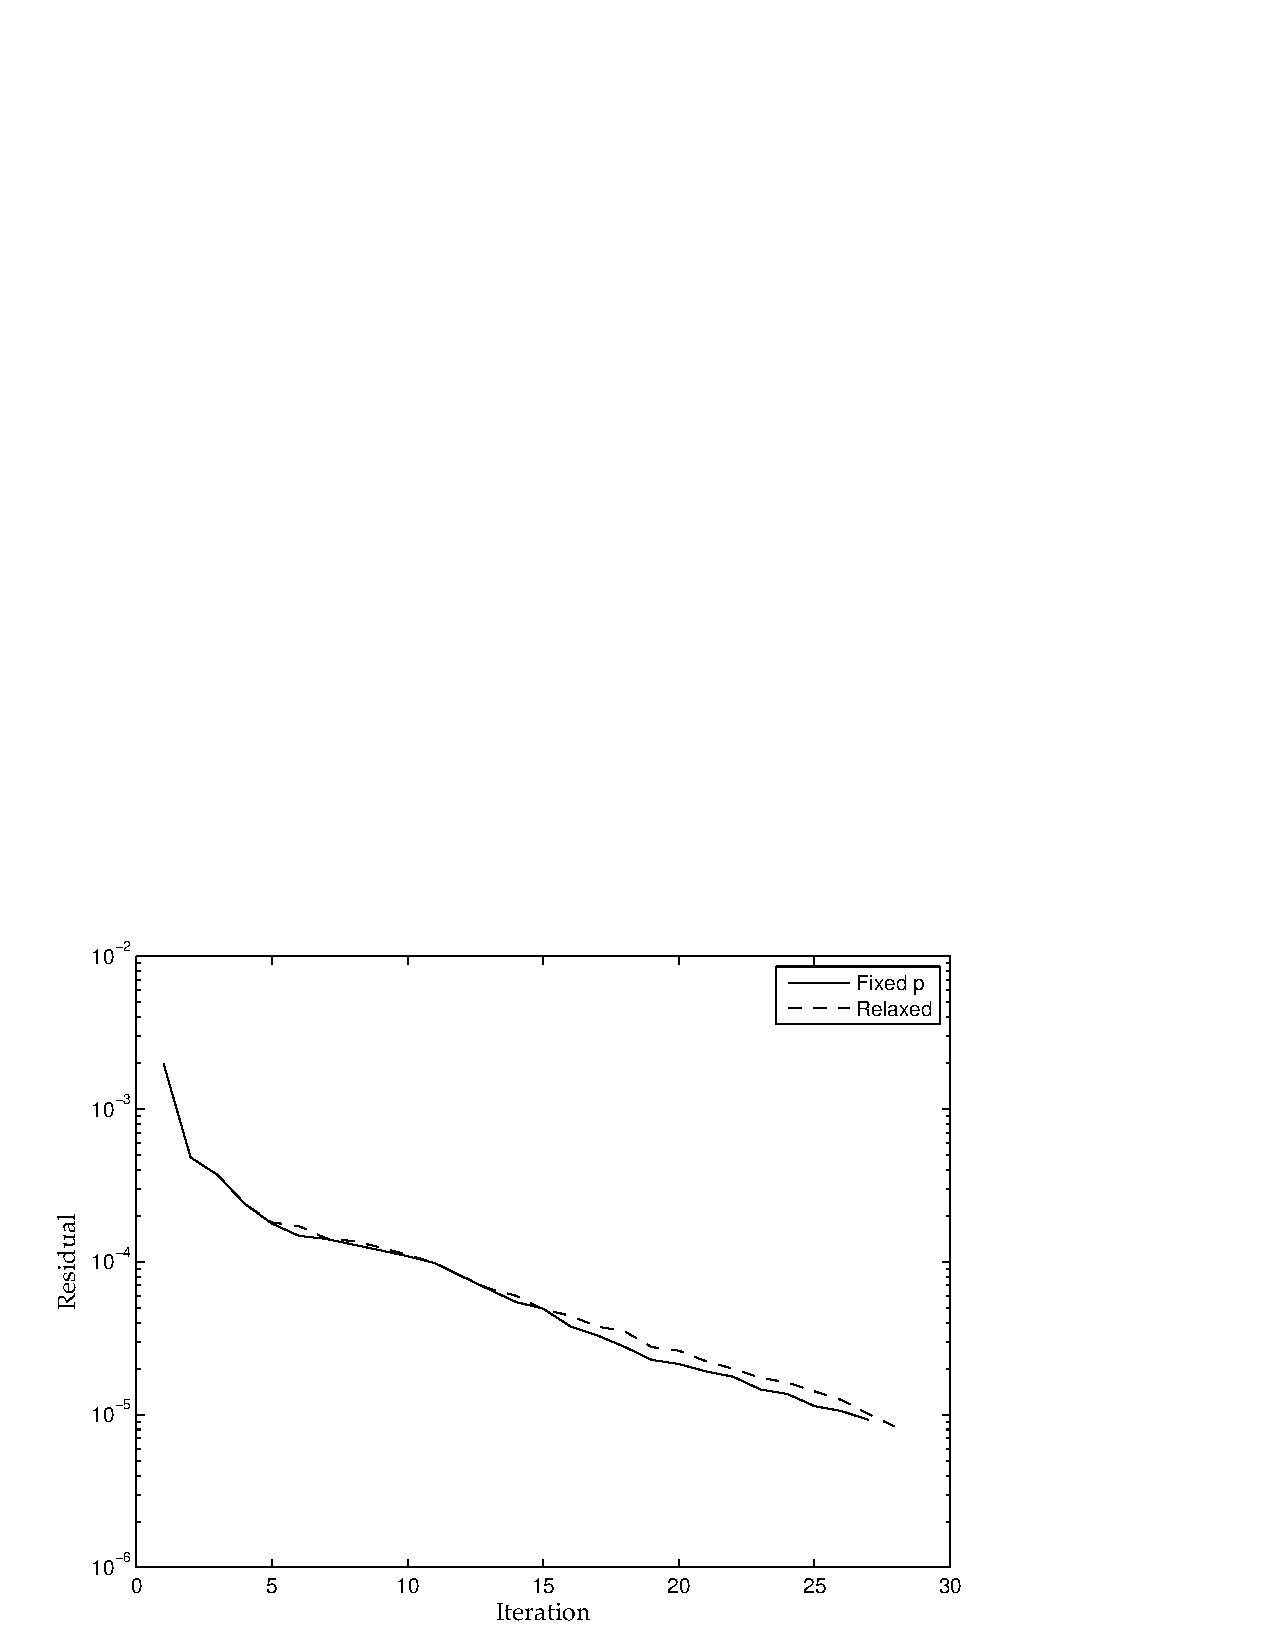
\includegraphics[width=14cm]{img/StokesResidualHistoryRelaxed.pdf}
	\caption{Residual history solving for surface traction on the surface of a sphere, $10^{-5}$ solver tolerance, $8192$ panels, $p=16$.}
	\label{fig:stokes_residual_history_relaxed}
\end{center}
\end{figure}

During this period of initial testing, we confirmed the departure from standard {\fmm} practice as regards to choosing $\ncrit$ and $p$ that we first encountered in \S\ref{sec:laplace_relaxation} for the Laplace equation. Traditionally, we would try to balance the amount of time spent on the near-field ({\ptop}) and far-field (dominated by {\mtol}). While this works well for the case where we keep $p$ constant, it requires an adjustment for the relaxed case. In order for the optimal time to solution, we actually want to balance near and far-fields for the value of $p$ we spend most time on --- in the majority of cases, this is \emph{the lowest instance of $p$}. Figure \ref{fig:stokes_relaxation_breakdown} shows the residual history of a solver over a sphere, along with the breakdown of {\ptop} and {\mtol} for each iteration.

During the verification of our relaxed solver, we encountered a new issue unseen for the Laplace equation in chapter \ref{chapter:laplace_bem}, the need to enforce a \emph{minimum $p$} in order to maintain accuracy. We ran extensive tests on the smallest value of $p$ that could be allowed within the relaxed solver, whilst still maintaining both accuracy and convergence properties. Some of these results are summarized in table \ref{tab:stokes_min_p}.

\begin{table}[htdp]
\begin{center}
\begin{tabular}{c|cc|cc|cc}
  & \multicolumn{2}{c|}{2048 panels} & \multicolumn{2}{c|}{8192 panels} & \multicolumn{2}{c}{32768 panels} \\
 $\pmin$ & Error & $it$ & Error & $it$ & Error & $it$ \\ \hline
  & & & & & & \\
 5 & $4.70\times 10^{-2}$ & 22 & $2.44\times 10^{-2}$ & 28 & $1.34\times 10^{-2}$ & 28 \\
  & & & & & & \\
 4 & $4.49\times 10^{-2}$ & 23 & $2.51\times 10^{-2}$ & 29 & $1.25\times 10^{-2}$ & 29 \\
  & & & & & & \\ 
 3 & $4.64\times 10^{-2}$ & 22 & $2.78\times 10^{-2}$ & 29 & $1.39\times 10^{-2}$ & 29 \\
  & & & & & & \\
 2 & $4.95\times 10^{-2}$ & 25 & $2.62\times 10^{-2}$ & 33 & $3.18\times 10^{-2}$ & 39 \\
  & & & & & & \\
 1 & $4.96\times 10^{-2}$ & 25 & $2.99\times 10^{-2}$ & 51 & $4.77\times 10^{-2}$ & 53 
\end{tabular}
\end{center}
\caption{Effect of $p_{\text{min}}$ on accuracy and convergence for Stokes flow around a sphere for differing values of $N$. Error is on the total drag force in the $x$-direction, $F_x$.}
\label{tab:stokes_min_p}
\end{table}%

These results show that as we discretize more finely, the value of $\pmin$ becomes ever more important. While for 2048 panels, the effect in terms of both accuracy and iteration count is small, it becomes more noticeable at 8192 panels -- with $\pmin = 1$ we require almost twice as many iterations to converge to our tolerance with respect to $\pmin=5$. With 32768 panels, the problems become even more noticeable, with accuracy severely affected at $\pmin=2$ and below. This loss of accuracy is so large that for $\pmin=1$ the error is almost $4\times$ worse than for $\pmin=5$.

Due to this behaviour, we choose to prioritize accuracy over some speed gains and use $\pmin=5$ for all further Stokes flow cases seen in this thesis. We will lose some potential speedups from iterations at even lower values of $p$, but for all cases tried in the course of the experimentation for this thesis, $\pmin=5$ has produced accurate results with good convergence properties.

\begin{figure}[h]
\begin{center}
	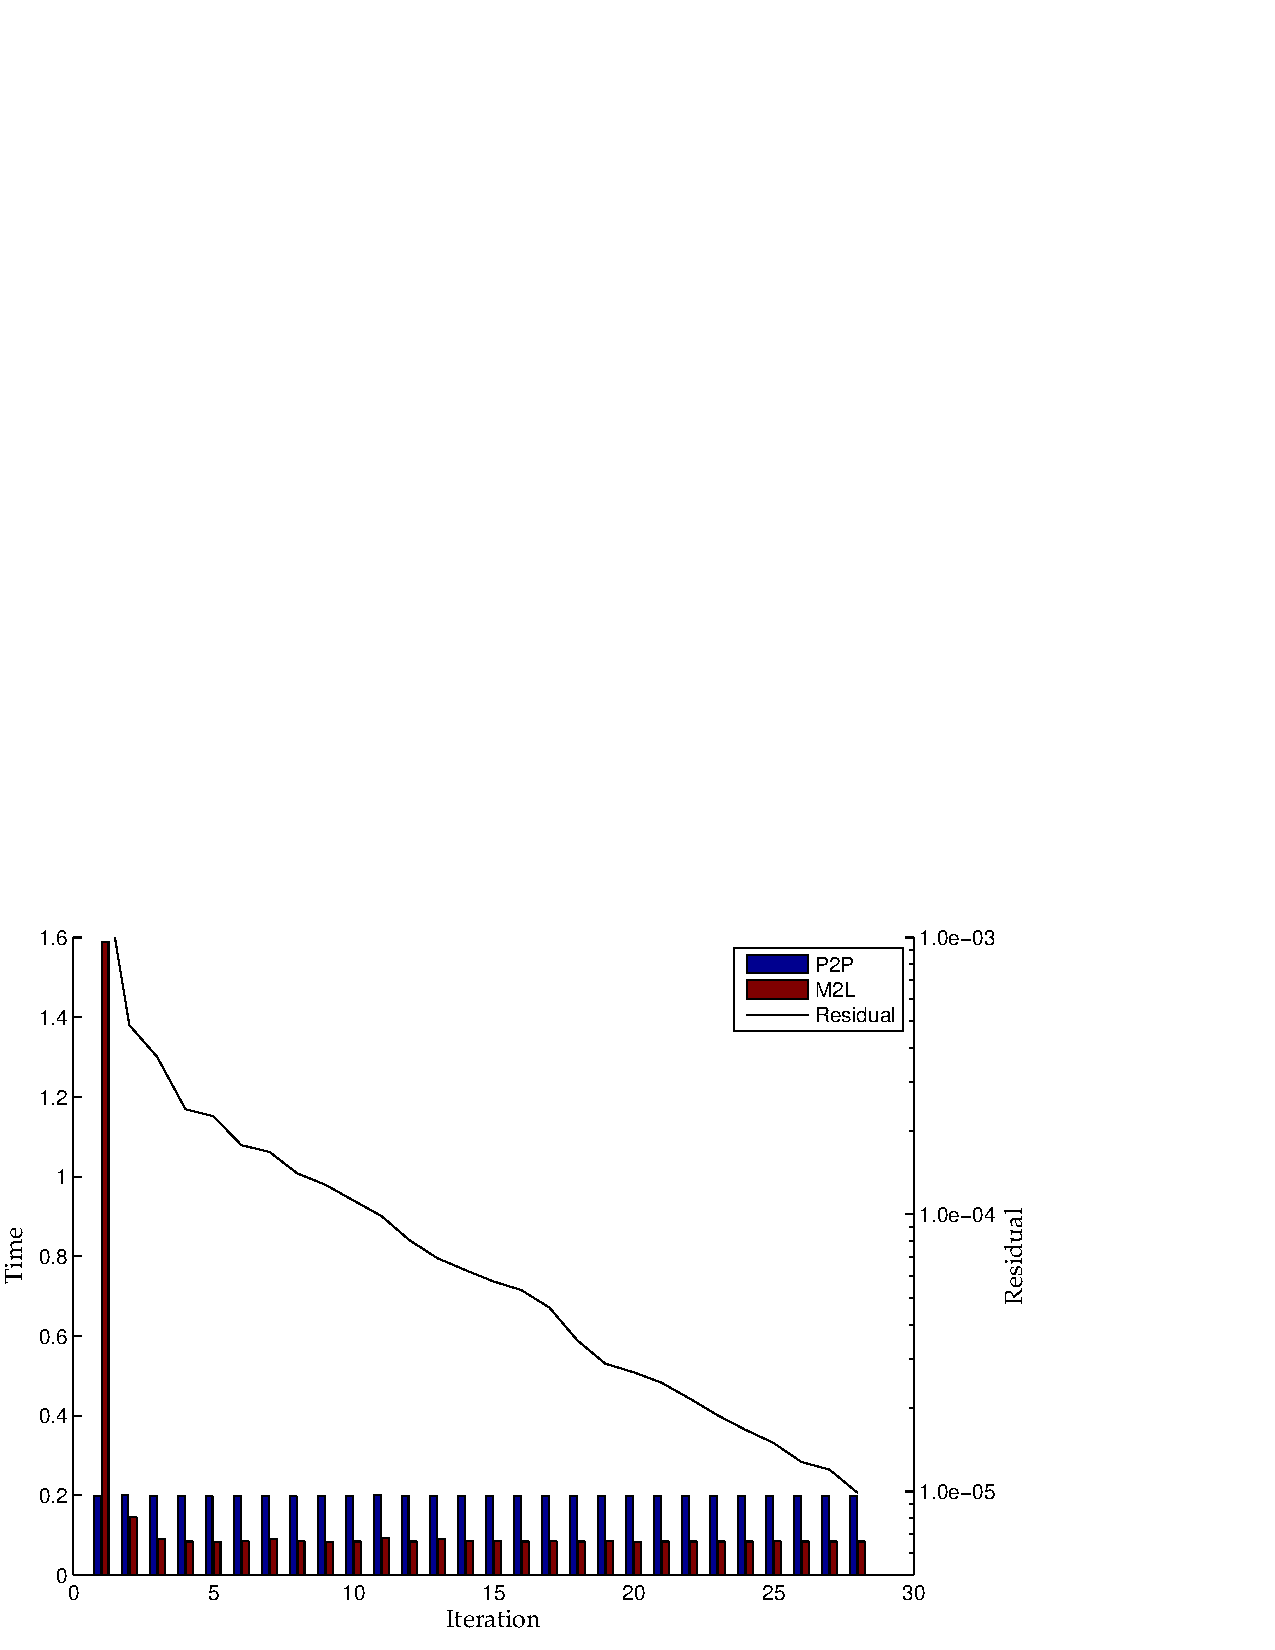
\includegraphics[width=14cm]{img/StokesRelaxationBreakdown.pdf}
	\caption{Residual history solving for surface traction on the surface of a sphere, with time breakdown between {\ptop} and {\mtol}. $10^{-5}$ solver tolerance, $8192$ panels, $p=16$.}
	\label{fig:stokes_relaxation_breakdown}
\end{center}
\end{figure}

The results shown in figure \ref{fig:stokes_relaxation_breakdown} indicate that we spend the vast majority of iterations at the minimum $p$, so, confirming our observation from chapter \ref{chapter:laplace_bem} and the Laplace equation, it is in our best interests to balance the computation for low $p$ case. In practise, this means setting $\ncrit$ to the lowest possible in order to maintain the accuracy of the {\fmm}, as the {\mtol} component becomes very fast at the lowest values of $p$.

After exploring the behavior of the relaxed solver, we can finally present speedup results. Figure \ref{fig:stokes_speedup} shows the speedup of the relaxed solver over keeping $p$ fixed for $N=2048$ to $131072$ (6144 to 393216 unknowns).

\begin{figure}[h]
\begin{center}
	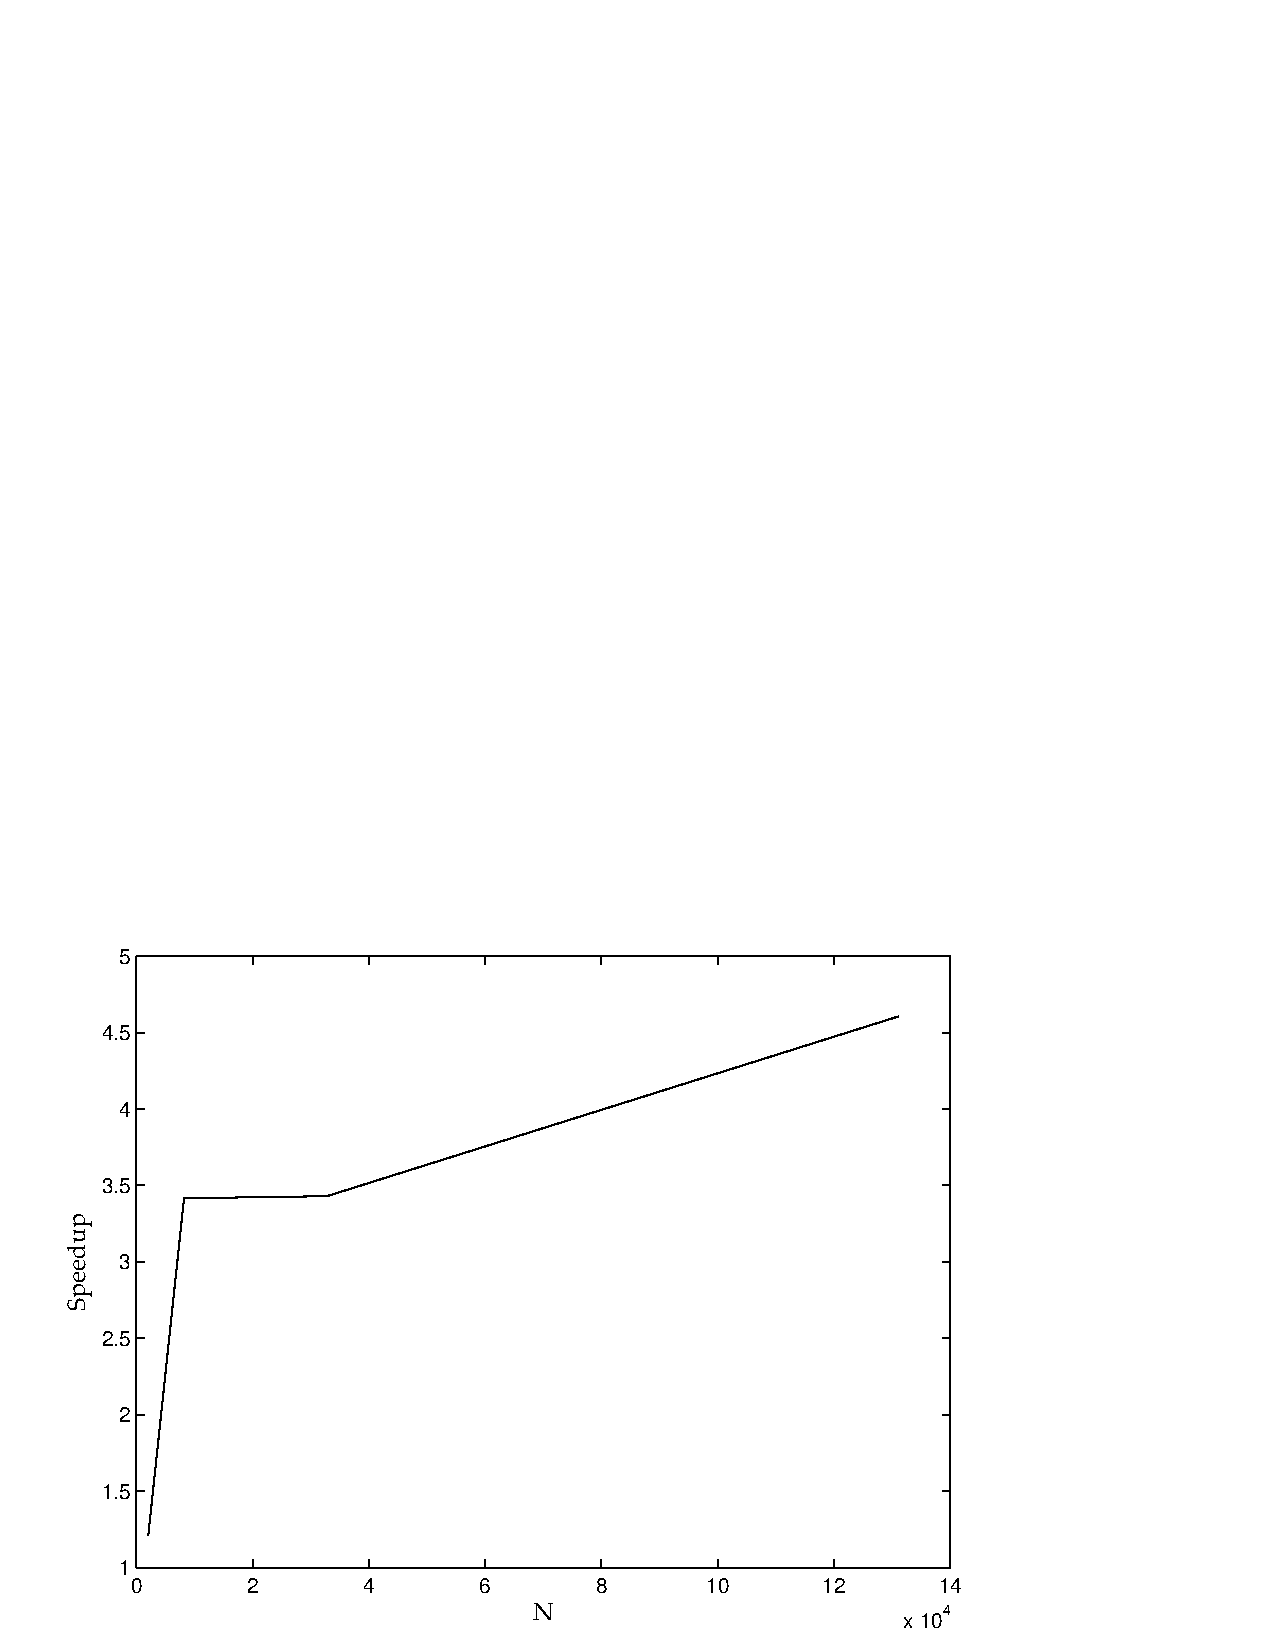
\includegraphics[width=14cm]{img/StokesSpeedup.pdf}
	\caption{Speedup for solving first-kind Stokes equation on the surface of a sphere, varying $N$. $10^{-5}$ solver tolerance, $p=16$. }
	%\caption{Residual history solving for surface traction on the surface of a sphere, with time breakdown between {\ptop} and {\mtol}. $10^{-5}$ solver tolerance, $8192$ panels, $p=16$.}
	\label{fig:stokes_speedup}
\end{center}
\end{figure}

These results demonstrate that our optimism about the potential of relaxed solvers for Stokse problems was clearly warranted. Speedups for problems of $8192$ panels and more are $3.5\times$ or greater, and as problem sizes grow, the speedup increased to greater than $4\times$. This additional speedup for large problems is due to the disparity in $\ncrit$ values needed for relaxed and fixed $p$ cases, and the use of the sparse matrix near-field form from \S\ref{sec:fmm_near_field} -- the higher $\ncrit$ for fixed $p$ problems prohibits the use of the significantly faster sparse matrix approach due to memory consumption.
 
\section{Conclusions}\label{sec:stokes_conclusions}

In this section of the thesis, we have extended the work from chapter \ref{chapter:laplace_bem} to the Stokes equations, a significantly more difficult problem. Our implementation has been shown to converge to the correct solution for a standard test case, and we have demonstrated that as predicted, the combination of high-accuracy and large iteration counts for this type of problem has resulted in good speedups from a relaxed solver, reducing the time-to-solution by a factor of $3-4\times$. Further to these performance results, we have also shown the importance of setting a minimum value of $p$, $\pmin$, that we cannot relax below, in order to maintain accuracy. For all tests performed, $\pmin=5$ was good for minimizing iteration counts while maintaining accuracy. For general problems, the choice of $\pmin$ may be more difficult, requiring either a conservative choice to ensure accuracy, or multiple experiments with varying values of $\pmin$ so that any changes in the solution can be observed.

\cleardoublepage

% -------------------------------------
% CHAPTER 7: Red Blood Cells
% -------------------------------------
%!TEX root = ../thesis.tex

\chapter{BEM with inexact GMRES for Red Blood Cell problems}\label{chapter:rbc}
\thispagestyle{myheadings}

\graphicspath{{RBC/}}

To show ``real-world'' performance, we choose an application closer to contemporary Stokes {\bem} research than flow past a sphere. The behavior of both flow past red blood cells (RBCs), in our case ethrocytes, and the effect of this flow on the cells themselves has prompted research based on a variety of methods, from traditional fluid solvers to boundary integral formulations like the one presented in this thesis. These studies are of particular use to the medical field --- by better understanding the microcirculation of blood, topics such as anti-coagulation therapy and stroke research would greatly benefit \cite{RahimianETal2010}. To summarize state-of-the-art in the boundary integral representation of RBCs, we briefly discuss 3 papers.

The first was an early attempt at a large-scale simulation \cite{zinchenko2003}, using $\O{1000}$ panels per elliptical cell (Vessicle) and utilizing a periodic domain of $\O{100s}$ of cells in order to approximate blood cells in plasma using an emulsion model. Extending this idea, the winner of the prestigious Gordon Bell prize in 2011 \cite{RahimianETal2010} used large numbers of low-definition elliptical vessicles ($\O{100}$ panels per cell) with a coupled Stokes and elasticity formulation to simulate blood drops -- the largest simulation was performed with 200 million cells, and 90 billion unknowns (velocity and forces). This corresponds to roughly 40 drops of blood. Finally, the simulation closest in capability to the work in this thesis involves 40 ethrocyte cells comprising of 7500 panels each \cite{Liu2009}. This experiment was non time-dependant, and did not involve any cell deformation, making it directly comparable to our work.

These experiments are characterized by their size --- the computational capacity required, the number of cells used and the amount of time taken for simulations. The application of a relaxation scheme would give the option of either reducing both the computational and time requirements, or performing experiments with more cells or the same amount, but better discretized cells. Both options would provide a significant gain in capability for any suitable code.

While research often includes deformation of the cells by using a linear elasticity {\bem} and unsteady flow to show the time-dependant evolution of cells in blood flow, we choose to demonstrate only the Stokes-flow part. The equations for linear elasticity can be treated in the same way as those for the Stokes equation --- we integrate over tensors, the result is a vector quantity, and we can use an {\fmm} to improve the scaling of $N$-body products by a decomposition into multiple harmonic {\fmm}s. Thus, speedups from relaxation for the purely Stokes problem can be viewed as analogous to speedups that would be required for both linear elasticity and the combined problem. Unsteady flow would involve repeated {\bem} solves of comparable or equal difficulty, so we can view any speedup for a single solve (single time-step) as applicable for every solve at every time-step.

%%%%%%%%%%%%%%%%%%%%%%%%%%%%%%%%%%%%%%%%%%%%%%%
%%%%%% GEOMETRY
%%%%%%%%%%%%%%%%%%%%%%%%%%%%%%%%%%%%%%%%%%%%%%%
\section{Geometry and Single Cell}

While there are many ways of obtaining a surface mesh for the ethrocyte, we choose a parameterization method \cite{kruger2012} in order to re-use our existing geometry creation routines for a sphere. The method is based on applying a simple transform to every vertex, such that a vertex, $v = v(x,y,z),\;x,y,z\in [-1,1]$ is transformed into $v' = v'(x',y',z(\rho'))$, where $x' = x\cdot r,\; y' = y\cdot r,\; \rho = \sqrt{x'^{2}+y'^{2}}$ and

\begin{equation}
	\label{eqn:rbc_parameterization}
	z(\rho) = \pm \frac{1}{2}\sqrt{1 - \left(\frac{\rho}{r}\right)^{2}}\left ( C_0 + C_2 \left(\frac{\rho}{r}\right)^{2} + C_4\left(\frac{\rho}{r}\right)^{4}\right ).
\end{equation}

In this form, the rotation axis of symmetry is along the $z$-axis, we choose the $\pm$ based on whether the original vertex has $\pm z$, and the constants are shown in table \ref{tab:rbc_parameterization_constants}:

\begin{table}[htdp]
\begin{center}
\begin{tabular}{c|c}
	Constant & Value \\ 
	& \\\hline
	& \\
	$r$ & $3.91\mu m$ \\
	& \\
	$C_0$ & $0.81\mu m$ \\ 
	& \\
	$C_2$ & $7.83\mu m$ \\
	& \\
	$C_4$ & $-4.39\mu m$
\end{tabular}
\end{center}
\caption{Constants for equation \eqref{eqn:rbc_parameterization}}
\label{tab:rbc_parameterization_constants}
\end{table}%

This formulation provides a smooth, well-resolved surface mesh, with triangles of relatively uniform size and shape, shown in figures \ref{fig:rbc512}, \ref{fig:rbc2048}.

\begin{center}
\begin{figure}[h]
	\subfloat[][512 panels]{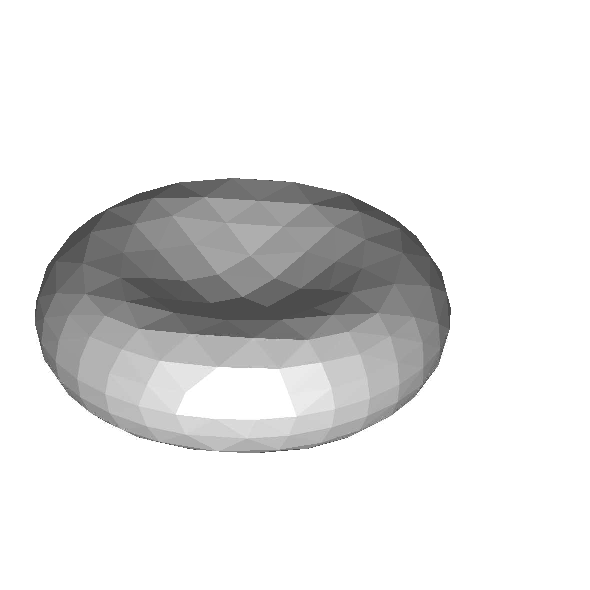
\includegraphics[width=7.5cm]{img/RBC512.pdf}\label{fig:rbc512}}\qquad
	\subfloat[][2048 panels]{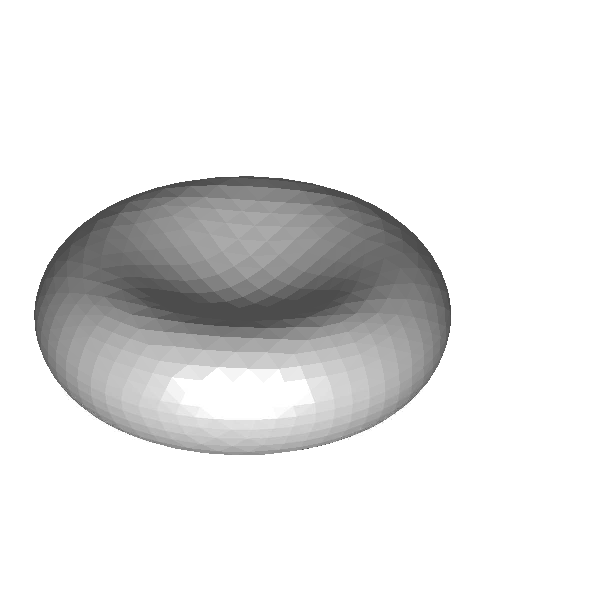
\includegraphics[width=7.5cm]{img/RBC2048.pdf}\label{fig:rbc2048}}\qquad
	\caption{Triangular discretizations of an ethrocyte, parameterized from a sphere.}
	\label{fig:glob_rbc}
\end{figure}
\end{center}

When placed in a flow with $U_x = 1,\; \mu=10^{-3}$, we obtain the traction force in the $x$-direction, shown in figure \ref{fig:stokes_rbc_traction}.

\begin{figure}[h]
\begin{center}
	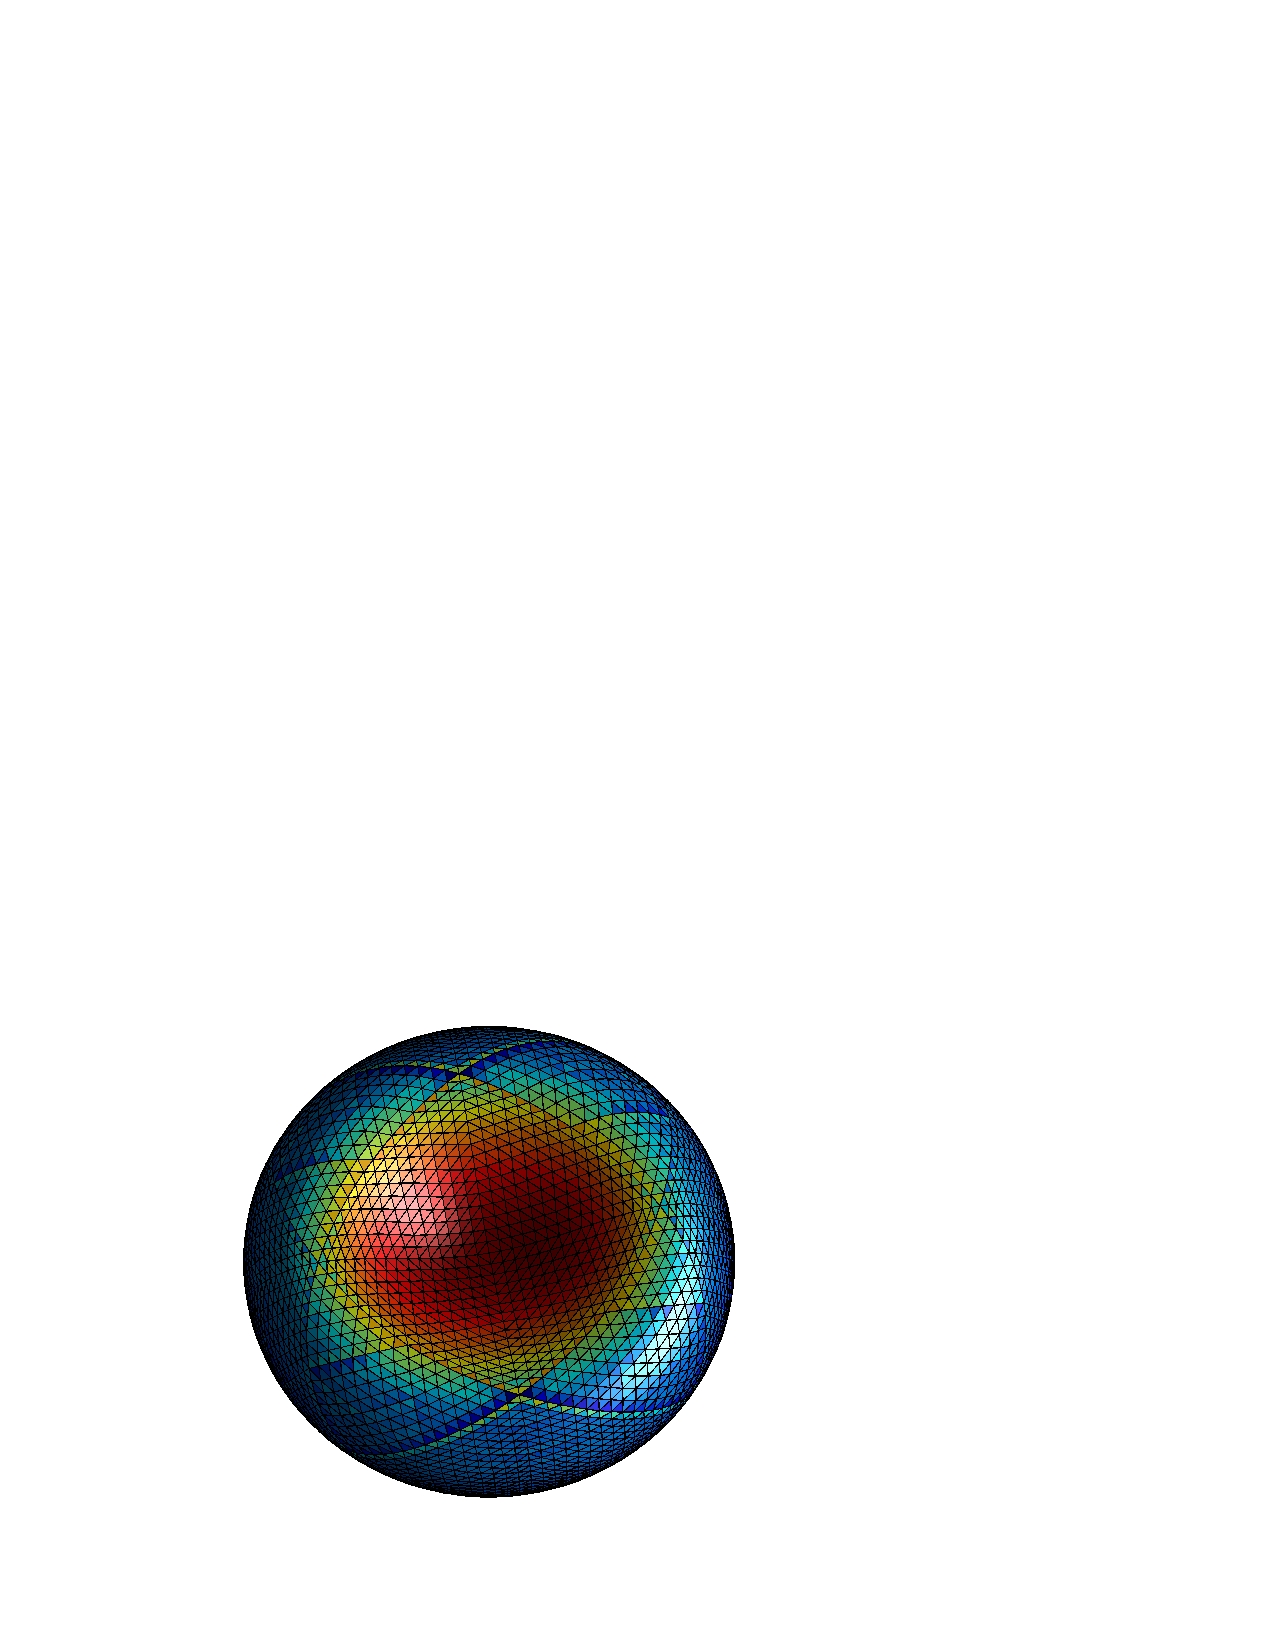
\includegraphics[width=14cm]{img/RBCTraction2.pdf}
	\caption{Traction force $t_x$ exerted in the $x$-direction on an Ethrocyte with 8192 panels, $p=16$, $\pmin=5$ solved to $10^{-5}$ tolerance}
	\label{fig:stokes_rbc_traction}
\end{center}
\end{figure}

While we do not have any kind of analytic expression for any of the flow quantities, we can still test the correctness of our method by checking if our calculated results converge as expected to some extrapolated value. As we tested the convergence of the drag force for convergence purposes with the sphere, it is a natural choice to use it for the ethrocyte as well. To obtain an extrapolated value for the drag, we use Richardson extrapolation \cite{roache1998}, choosing the calculated drag force from $3$ different meshes, with a constant refinement factor, $C$ (in this case $4$). Then, to calculate the extrapolated force value, $\bar{f}$, we  use the formula below, with $f_1$ being the coarsest mesh, and $f_3$ the finest.

\begin{equation}
	\bar{f} = \frac{f_1f_3-f_2^{2}}{f-1 -2f_2+f_3}
\end{equation}

Another useful quantity we obtain from this procedure, is the \emph{observed order of convergence}, a measure of the true convergence obtained with our method. Denoted by $p$, this is given by

\begin{equation}
	p = \frac{\ln{\left(\frac{f_2-f_1}{f_3-f_2}\right)}}{\ln{C}}.
\end{equation}

Using the mesh, $f_x$ value pairs given in table \ref{tab:rbc_richardson_values}, we calculate the converged drag force to be $f_x = -0.0834$, and the observed order of convergence to be $0.481$. This shows both that our solution is converging spatially to a value, and that the rate of convergence is $\O{\sqrt{N}}$, the same as observed for the sphere test case.

\begin{table}[htdp]
\begin{center}
\begin{tabular}{c|c}
	$N$ & $f_x$ \\
	& \\\hline
	& \\
	$512$ & $-0.059$ \\
	& \\
	$2048$ & $-0.071$ \\ 
	& \\
	$8192$ & $-0.077$ \\
%	& \\
%	$32768$ & $-0.080$
\end{tabular}
\end{center}
\caption{Values of mesh size and calculated drag force for convergence study}
\label{tab:rbc_richardson_values}
\end{table}%

To further illustrate this important result, we can use the extrapolated $f_x$ as an ``exact value'' in order to calculate errors at each of our mesh points. This error is plotted in figure \ref{fig:rbc_extrapolated_convergence}, where the first 3 points were used to calculate the extrapolated value, and the final, largest point was used as a test.

\begin{figure}
\begin{center}
	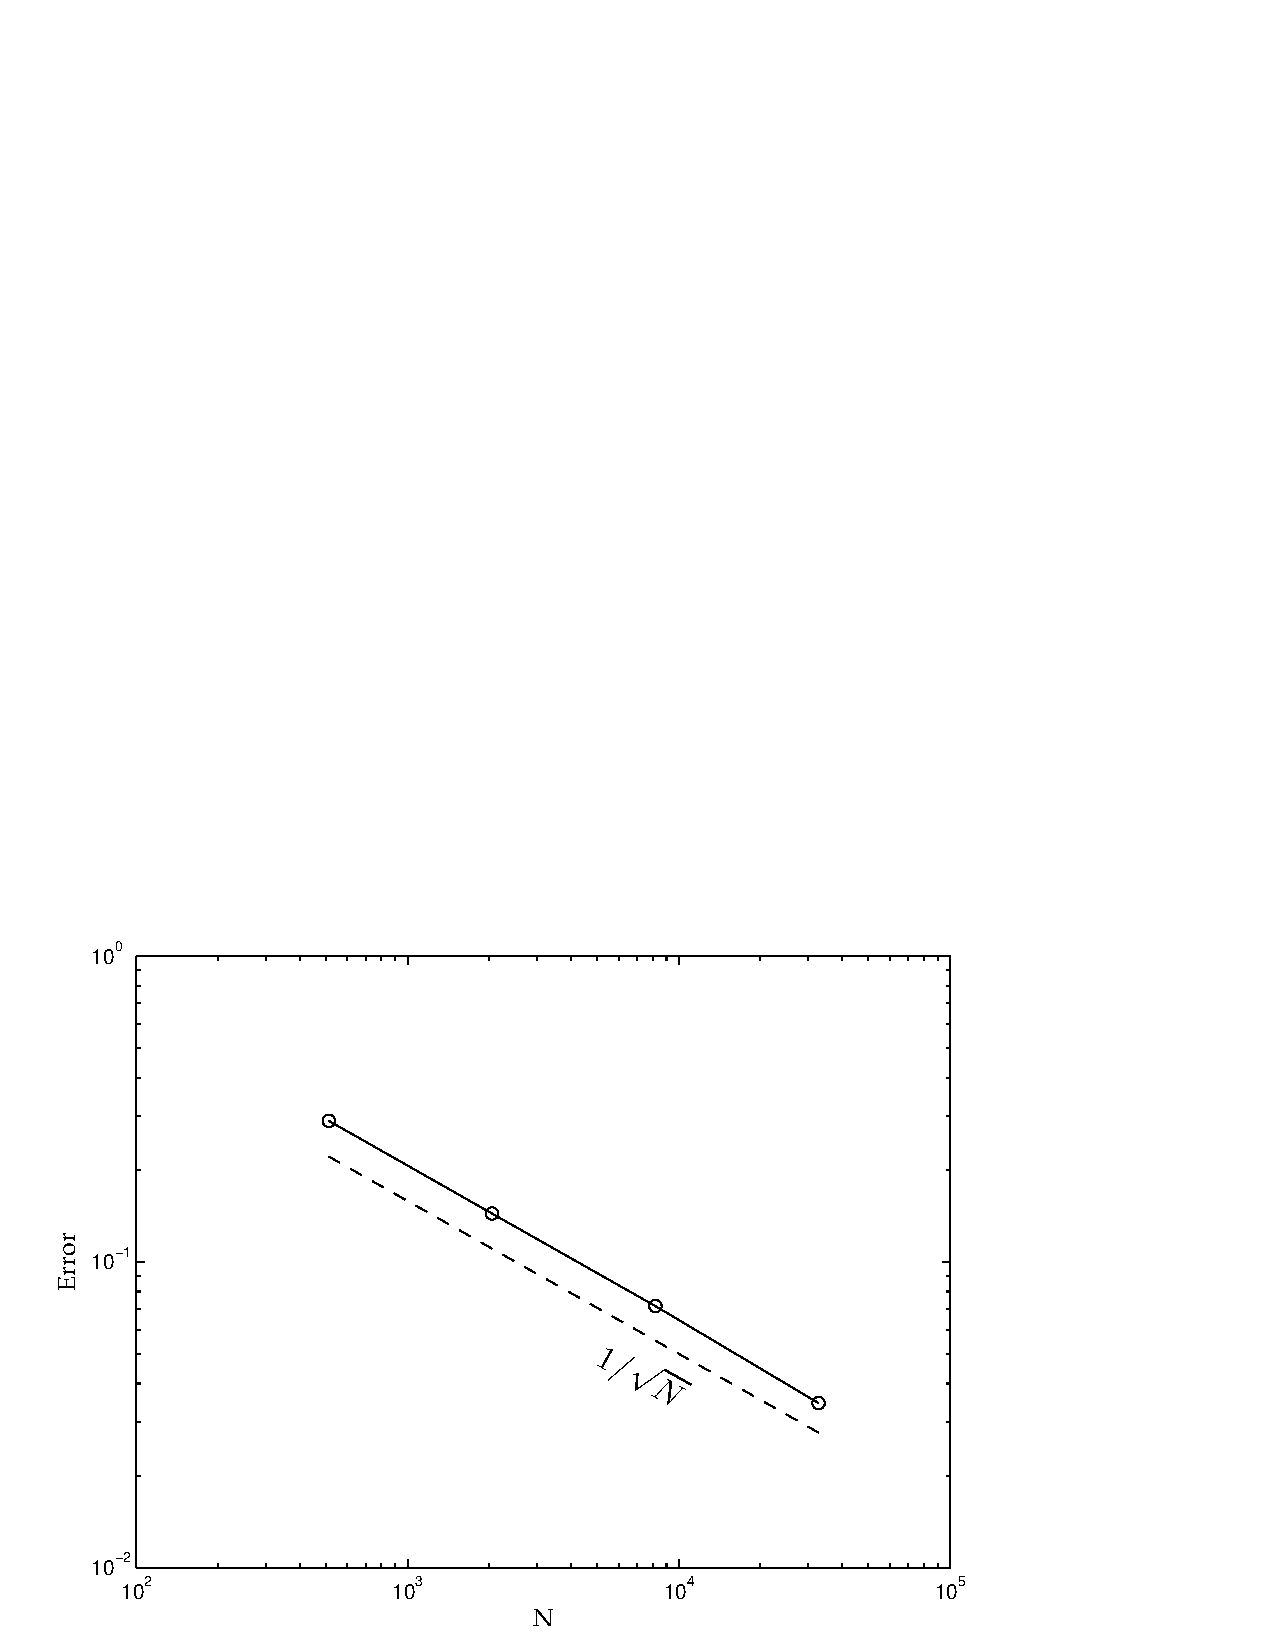
\includegraphics[width=12.5cm]{img/ExtrapolatedConverged.pdf}
	\caption{Observed convergence for Ethrocyte with respect to extrapolated value}
	\label{fig:rbc_extrapolated_convergence}
\end{center}
\end{figure}

This result shows that we are observing the same order or convergence for the ethrocyte case as for the simpler sphere --- this gives us more confidence that our {\fmmbem} solver is behaving as expected.

%%%%%%%%%%%%%%%%%%%%%%%%%%%%%%%%%%%%%%%%%%%%%%%
%%%%%% MULTIPLE CELLS
%%%%%%%%%%%%%%%%%%%%%%%%%%%%%%%%%%%%%%%%%%%%%%%
\section{Multiple Cells}\label{sec:multiple_cells}

While the flow around a single ethrocyte is more interesting than flow over a sphere, it is still not of much interest. For a more substantial problem, we look at multiple ethrocytes together, representing a single instant of blood flow in an artery / vein.

Due to the nature of the {\bem} formulation, the only difference between a single ethrocyte and multiple ones, is that the total number of panels is going to increase, and if we were to be using a dense matrix instead of the {\fmm}, it would increase in size from $(3N)\times (3N)$ to $(3N_cN)\times (3N_cN)$, where $N_c$ is the number of cells we choose to use. In the {\fmm} case, we simply have more source and target panels, and due to the $\O{N}$ scaling, the time taken for each matrix-vector product should increase linearly.

In order to generate an interesting combination of cells, we repeatedly take a single ethrocyte, then apply a random rotation and shift in space, ensuring that cells do not overlap. An example of this is shown in figure \ref{fig:multiple_cells}.

\begin{figure}
\begin{center}
	% do this image horizontally
	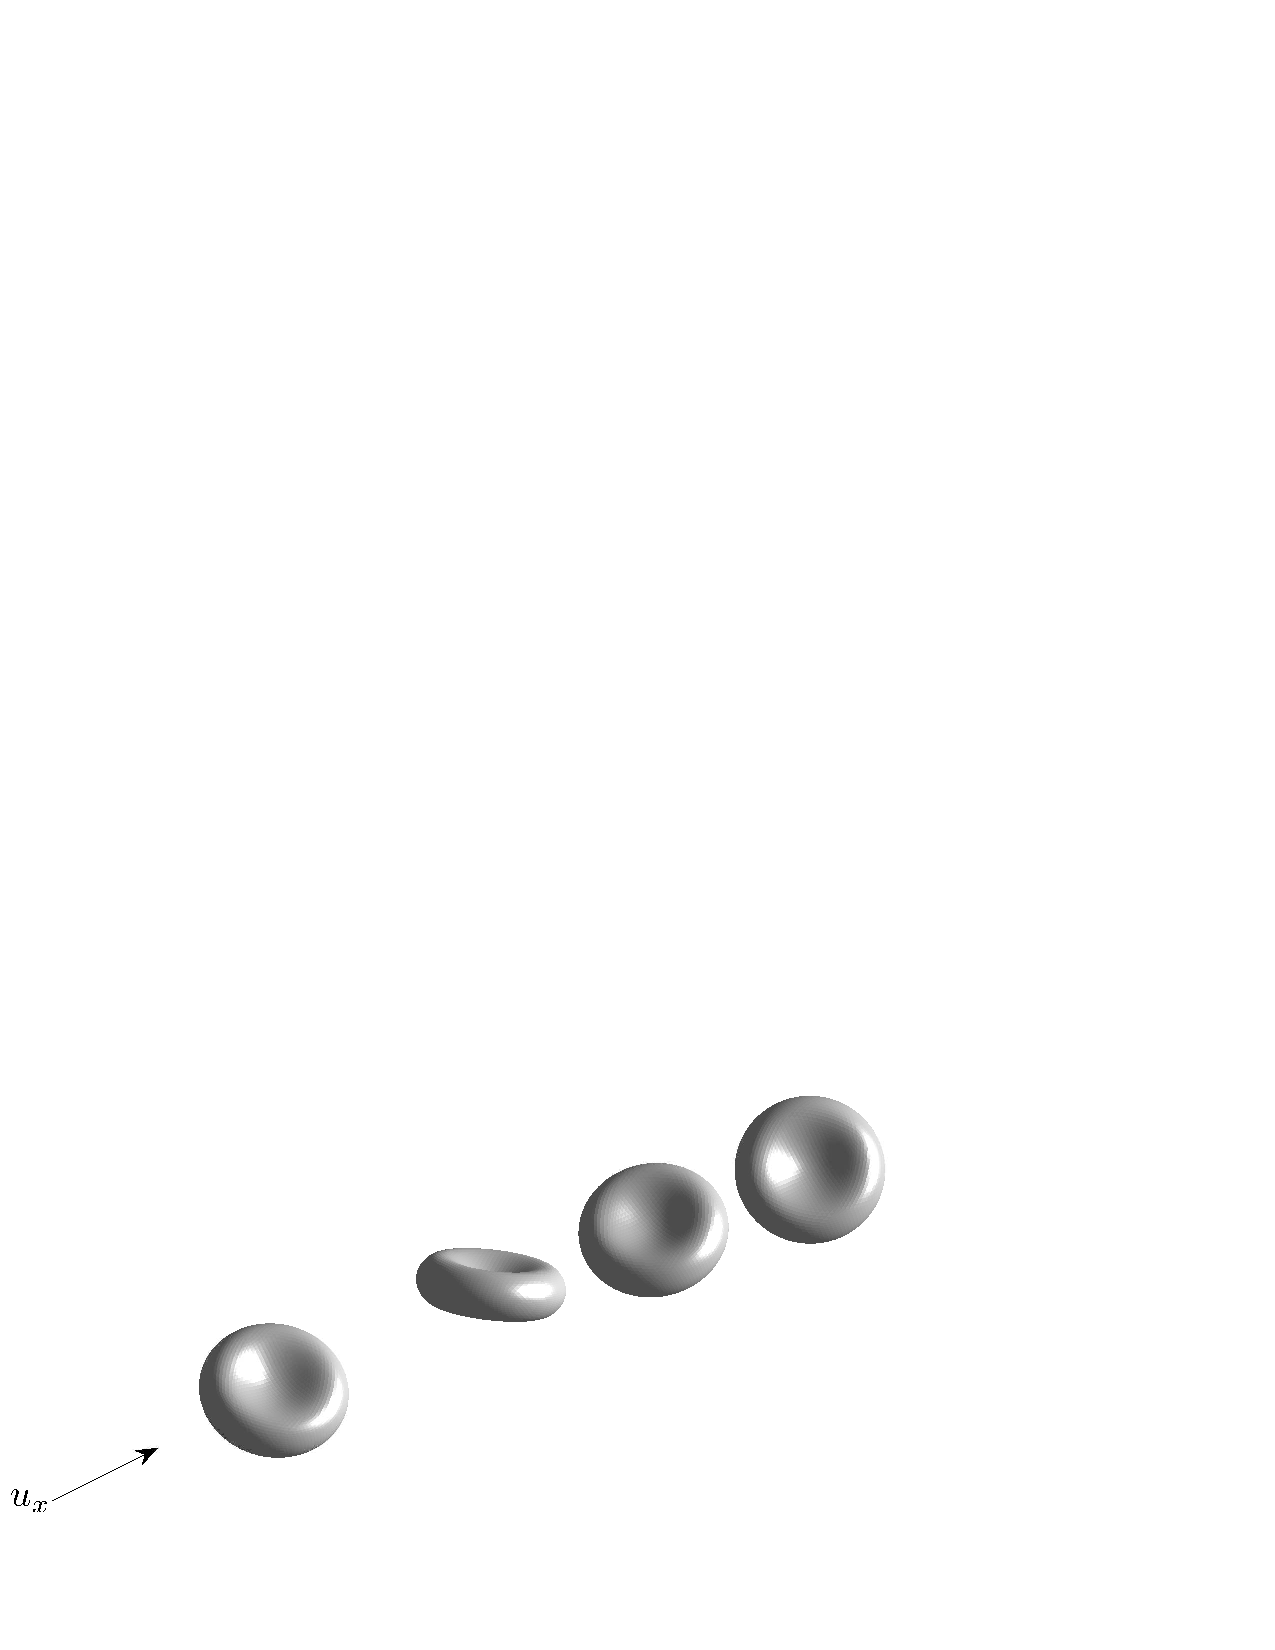
\includegraphics[width=14cm]{img/4Cells_arrow.pdf}
	\caption{Example surfaces for 4 Ethrocytes in fluid}
	\label{fig:multiple_cells}
\end{center}
\end{figure}

Given our ability to generate geometries with arbitrary numbers of cells, we can perform a number of interesting experiments. First, we study the properties of the resulting linear system (conditioning of the system), especially how the number of iterations changes as we increase $N_c$. Next, we examine the benefits of both preconditioners and relaxation (and combinations of both) on a non-trivial problem.

%%%%%%%%%%%%%%%%%%%%%%%%%%%%%%%%%%%%%%%%%%%%%%%
%%%%%% CONVERGENCE PROPERTIES
%%%%%%%%%%%%%%%%%%%%%%%%%%%%%%%%%%%%%%%%%%%%%%%
\subsection{Convergence Properties}\label{sec:convergence_properties}

As we move from a single ethrocyte to many, we might suspect that the resulting linear system would become increasingly harder to solve. This can result from the fact that the system has increased in size by a factor of the number of cells, or from the natural assumption that as we add cells that are disconnected from each other, it becomes tougher to solve the system.

We would prefer to investigate this topic by calculating the condition number of actual problems, but for problem sizes that would be interesting ($8192$ panels / cell), the amount of memory required to calculate the condition would be very large. For instance, the aforementioned $8192$ panel case gives a dense matrix with $6\times 10^{8}$ entries, taking $4.6\text{GB}$ in double precision. Raising the number of panels to 32768, we have $9.7\times10^{9}$ entries in our matrix, taking $73.7\text{GB}$ in double precision, a prohibitive amount. 

While there has been some theoretical work on the condition number of matrices arising from 2D {\bem} problems, \cite{DijkstraMattheij06,dijkstramattheij2007}, and some numerical notes involving condition numbers for 3D MEMS problems (Stokes) \cite{frangi2005}, there are no analytical formulations to approximate the condition number for 3D Stokes, and the problems we are interested in are too large to produce a dense matrix representation and directly obtain the condition number. Due to these restrictions, we choose to approach this problem in terms of problem size and the number of iterations required to obtain a solution with a desired residual, using the iteration count as a proxy to the condition number.

First, as a baseline, we will look at the iterations required to solve the system for a single ethrocyte, whilst refining the surface mesh.

\begin{figure}
\begin{center}
	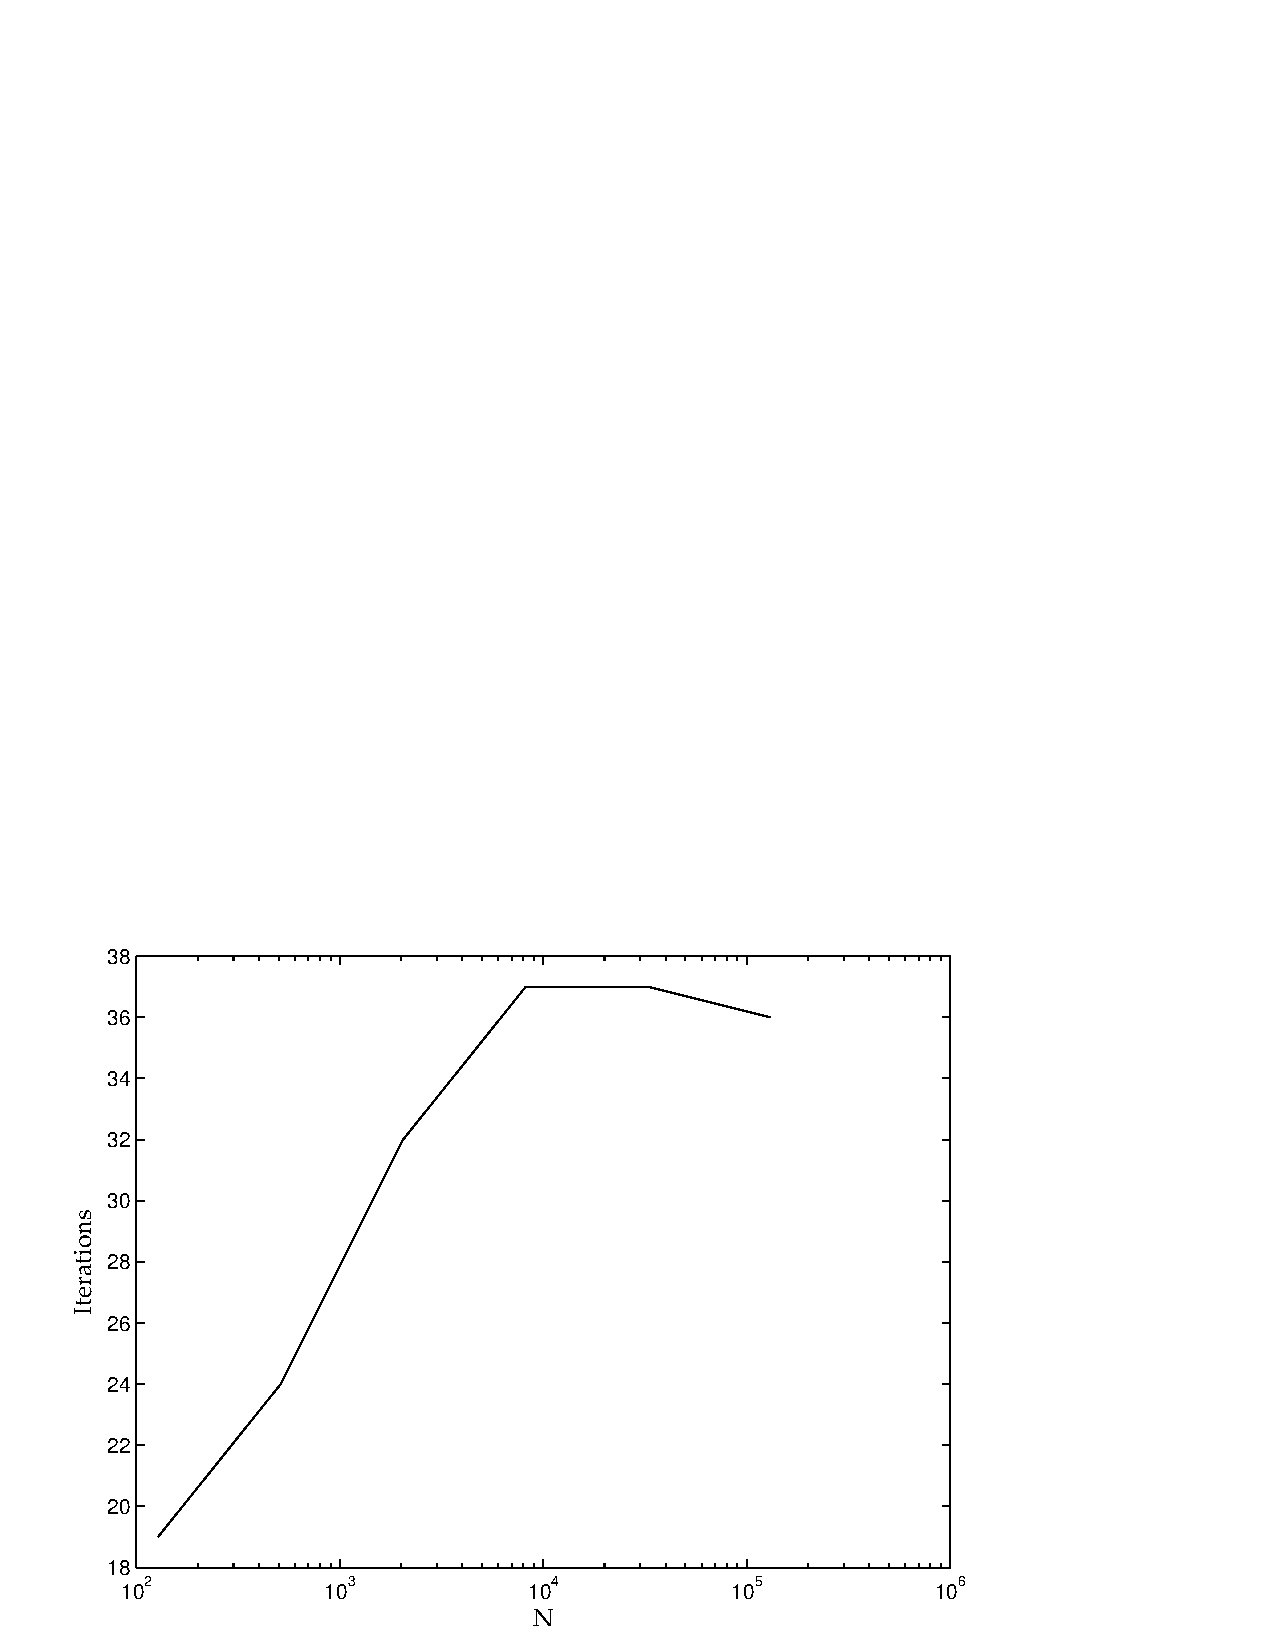
\includegraphics[width=12cm]{img/StokesSingleCellIterations.pdf}
	\caption{Iterations for Ethrocyte system to converge. $p = 16$, desired residual $10^{-5}$}
	\label{fig:single_cell_iterations}
\end{center}
\end{figure}

In figure \ref{fig:single_cell_iterations} we can see that as we increase from $128$ panels to $8192$, the number of iterations needed increases from $19$ to $37$, while as we further refine the mesh up to $131,072$ panels we see the number of iterations flatten out. This implies that beyond a certain point, the condition number of our matrix stops increasing, although without being able to test a larger system, we cannot confirm this. % [[[ IS THIS ACTUALLY TRUE??? ]]].

Now that we know how the convergence behaviour changes with respect to the number of panels per ethrocyte, we can look at how it changes with respect to multiple cells. We take advantage of the nature of our geometry creation (that is, the refinement factor is 4) to both test how the convergence changes as we increase the number of cells, as well as the effect of the number of panels per cell. In all cases $p = 16,\;p_{\text{min}} = 5$ and the solver tolerance is set to $10^{-5}$.

\begin{figure}
\begin{center}
	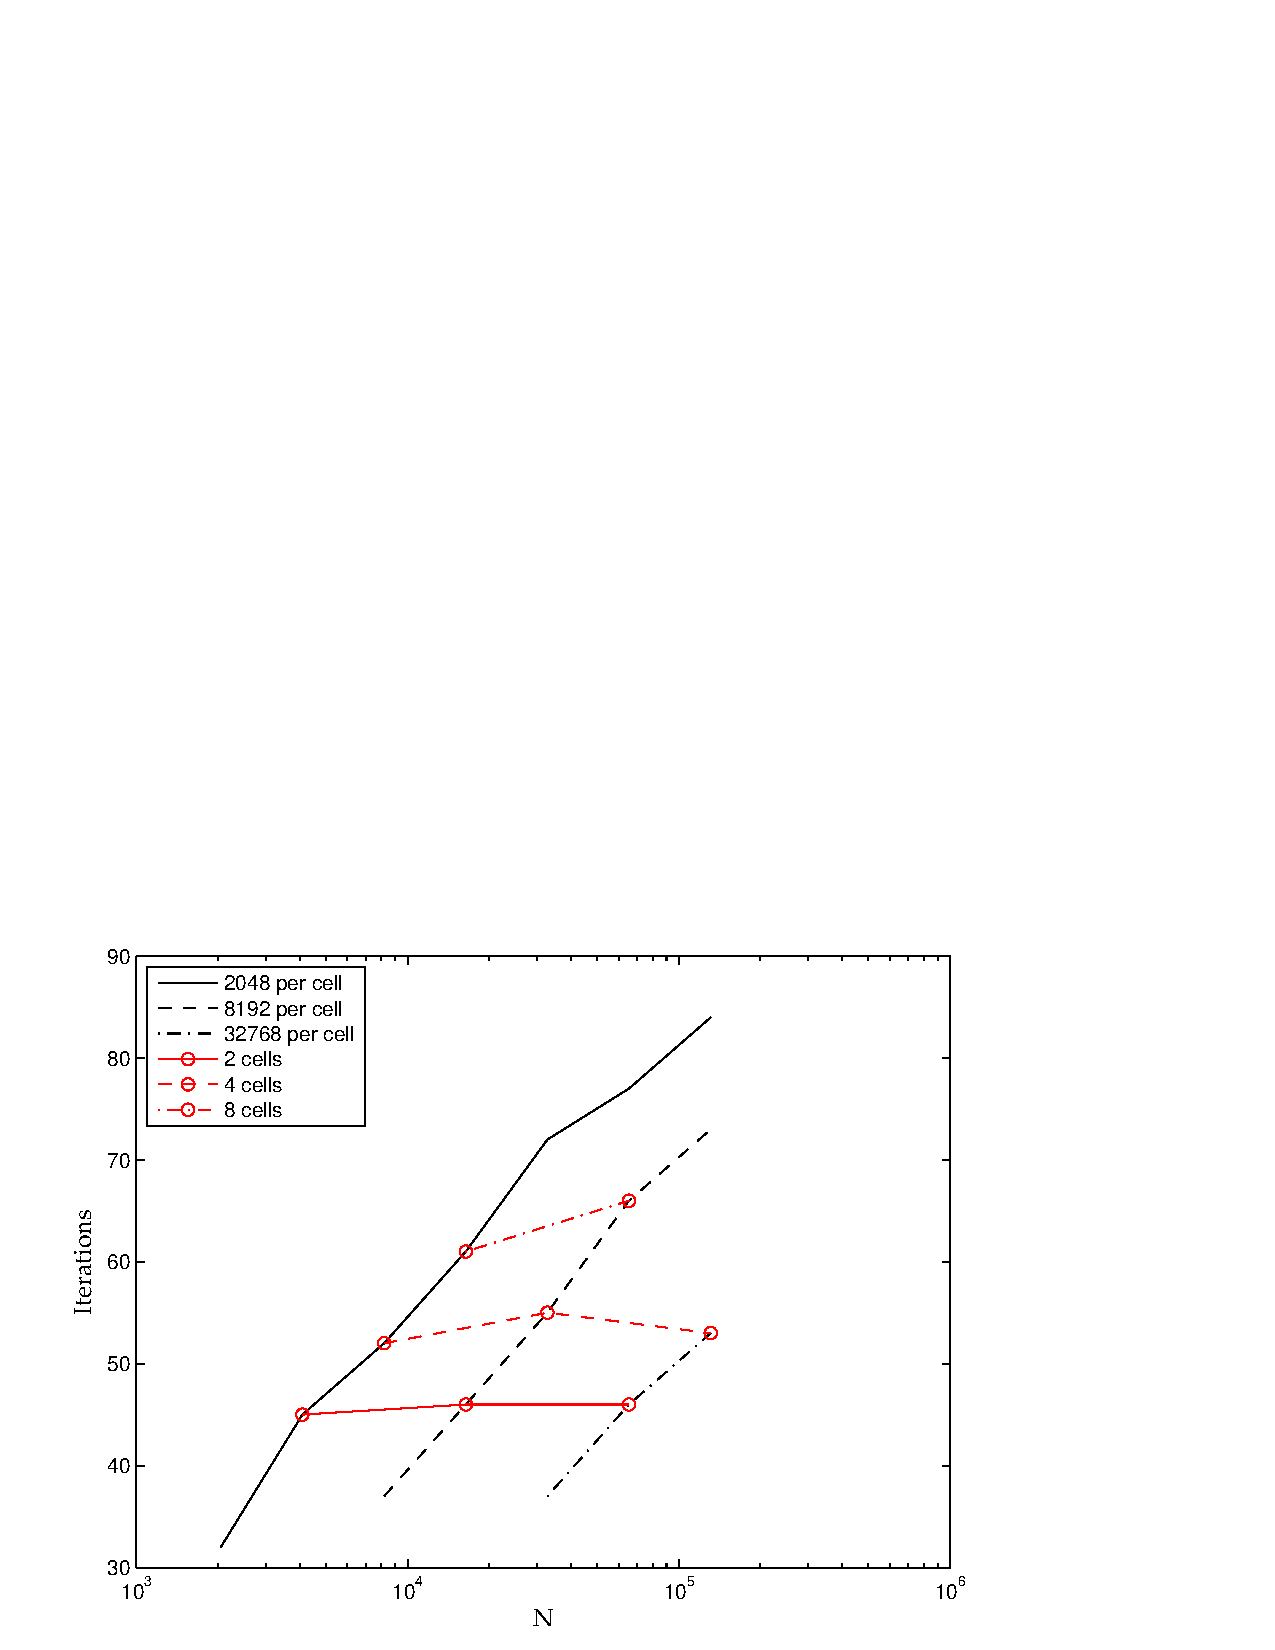
\includegraphics[width=11.5cm]{img/StokesMultipleCellsIterations.pdf}
	\caption{Iterations for system from multiple Ethrocyte to converge. $p = 16$, desired residual $10^{-5}$}
	\label{fig:multiple_cell_iterations}
\end{center}
\end{figure}

Figure \ref{fig:multiple_cell_iterations} shows how the number of iterations needed to converge changes with respect to the number of cells used and with respect to the number of panels per cell. In all 3 cases, $2048,\;8192$ or $32768$ panels per cell, we see a sharp increase in the number of iterations as the number of cells increases. Interestingly, if we look at the number of iterations required for a set number of cells, they are very similar for each case -- it makes little difference how many panels comprise each cell, the convergence properties are dominated by the number of cells. For instance, the system for 2 cells takes 45, 46 and 46 iterations for 2048, 8192 and 32768 panels per cell. Similarly, for 4 cells, 52, 55 and 53 iterations were needed for the analogous cases.

This is encouraging for the use of relaxation, as state-of-the-art simulations often involve 40 or more ethrocytes \cite{Liu2009,RahimianETal2010}, implying that we are likely to require a large number of iterations, potentially $\O{100}$, giving large potential gains in speed.

%%%%%%%%%%%%%%%%%%%%%%%%%%%%%%%%%%%%%%%%%%%%%%%
%%%%%% RELAXATION
%%%%%%%%%%%%%%%%%%%%%%%%%%%%%%%%%%%%%%%%%%%%%%%
\subsection{Relaxation}\label{sec:stokes_ethrocyte_relaxation}

Now that we have established the convergence properties of systems involving ethrocytes, we start to look at the advantages of using a relaxation scheme. With the results shown in figures \ref{fig:single_cell_iterations} and \ref{fig:multiple_cell_iterations}, we expect a large number of iterations to be needed in all cases. In addition to this, from figure \ref{fig:stokes_relaxation_breakdown} in our experiments on a spherical object, we expect to spend large numbers of iterations at a smaller value of $p$. Finally, figure \ref{fig:stokes_relaxation_breakdown}, shows the decrease in time for the far-field calculation when we reach our minimum $p$.

Combining these 3 observations, we can expect savings from applying a relaxation scheme for a single ethrocyte, with the gains increasing as a function of the number of cells. In all comparisons, the best parameters will be used -- for non-relaxed runs the near and far-field evaluations will be as balanced as possible, while for relaxed tests parameters will be chosen to give the shortest runtime. In every case we only look at the time taken in the solution phase (within the {\gmres} solver) as the setup (including generating the right-hand-side of the linear system) is 1) amortized over the total run, and 2) always performed at high-precision, so the behavior is identical for relaxed and fixed-$p$ cases. Small problems will not be tested, as the fastest solution will also be using a direct method, which inherently cannot use relaxation.

All experiments were performed with the settings described in table \ref{tab:cells_relaxation_settings}.

\begin{table}[h]
\begin{center}
\begin{tabular}{c|c}
 Variable & Setting \\ 
 & \\ \hline
 & \\
 $p_{\text{initial}}$ & $16$ \\
 & \\
 $p_{\text{min}}$ &  $5$ \\
 & \\
 solver tolerance & $10^{-5}$ \\
 & \\
 Near-field & Sparse matrix \\
 & \\
 Threads & $4$ \\
 & \\
 Solver & {\gmres} \\ 
 & \\
 Preconditioner & None
 
\end{tabular}
\end{center}
\caption{Ethrocyte relaxation test settings}
\label{tab:cells_relaxation_settings}
\end{table}%

Looking at the results in \ref{tab:single_cell_relaxation_results}, we see that we obtain a consistent $3-4\times$ speedup over non-relaxed results. The outlying result for $131072$ panels is due to being unable to use the significantly faster sparse-matrix representation of the near field. The variation in the other speedup numbers is a natural result of the behaviour of the {\fmm} when we choose different values of $\ncrit$ (and generate different octrees).

These results backup our original assumption that due to the combination of high numbers of iterations largely spent at low values of $p$, and the large savings from using that low $p$, we should see large time savings. Combining this observation with the known significant increase in iterations for the multiple ethrocyte case (\ref{fig:multiple_cell_iterations}), we expect to see time savings of a similar, if not greater degree.

\begin{table}[htdp]
\begin{center}
\begin{tabular}{c|c|c|c|c|c|c}

 & & \multicolumn{2}{c|}{Non-relaxed} & \multicolumn{2}{c|}{Relaxed} \\
 & & \multicolumn{2}{c|}{} & \multicolumn{2}{c|}{} \\
 N & \# unknowns & $\ncrit$ & $t_{\text{solve}}$ & $\ncrit$ & $t_{\text{solve}}$ & Speedup \\
 & & & & & \\ \hline
 & & & & & \\
 2048 & 6144 & 200 & 44.5 & 100 & 11.0 & 4.05 \\
 & & & & & \\
 8192 & 24576 & 400 & 177 & 150 & 52.4 & 3.37 \\
 & & & & & \\
 32768 & 98304 & 400 & 848 & 150 & 223 & 3.80 \\
 & & & & & \\
 131072 & 393216 & 600 & 6386\footnotemark[1] & 150 & 874 & 7.31\footnotemark[1] \\
 & & & & & \\
	
\end{tabular}
\end{center}
\caption{Single Ethrocyte relaxation test results, performed with initial $p=16$, $\pmin=5$, solved to $10^{-5}$ tolerance.}
\label{tab:single_cell_relaxation_results}
\end{table}%

\footnotetext[1]{Due to memory restrictions, the sparse-matrix representation of the near-field could not be used, resulting in a much slower {\ptop} evaluation}

%\begin{landscape}
%\begin{table}[htdp]
%\begin{center}
%\begin{tabular}{c|cccccc|cccccc|cccccc|}
%
%& \multicolumn{6}{c}{2048 panels / cell} & \multicolumn{6}{c}{8192 panels / cell} & \multicolumn{6}{c}{32768 panels / cell} \\
%& & \multicolumn{2}{c}{Non-relaxed} & \multicolumn{2}{c}{Relaxed} & & & \multicolumn{2}{c}{Non-relaxed} & \multicolumn{2}{c}{Relaxed} & & & \multicolumn{2}{c}{Non-relaxed} & \multicolumn{2}{c}{Relaxed} & \\
%N & $N_c$ & $\ncrit$ & $\tsolve$ & $\ncrit$ & $\tsolve$ & speedup & $N_c$ & $\ncrit$ & $\tsolve$ & $\ncrit$ & $\tsolve$ & speedup & $N_c$ & $\ncrit$ & $\tsolve$ & $\ncrit$ & $\tsolve$ & speedup \\ \hline
%& & & & & & & & & & & & & & & & & & \\
%2048 & 1 & 200 & 44.5 & 100 & 11.0 & 4.05 & \multicolumn{6}{c}{---} & \multicolumn{6}{c}{---} \\ 
%& & & & & & & & & & & & & & & & & & \\
%8192 & 4 & 200 & 236 & 150 & 59.8 & 3.95 & 1 & 400 & 177 & 150 & 52.4 & 3.37 & \multicolumn{6}{c}{---} \\
%& & & & & & & & & & & & & & & & & & \\
%32768 & 16 & 400 & 1261 & 150 & 331 & 3.81 & 4 & 400 & 1375 & 150 & 315 & 4.37 & 1 & 400 & 848 & 150 & 223 & 3.80 \\
%& & & & & & & & & & & & & & & & & & \\
%131072 & 64 & - & - & 100 & 1606 & - & 16 & - & - & 100 & 1681 & - & 4 & - & - & - & - & - \\
%
%	
%\end{tabular}
%\end{center}
%\caption{Multiple Ethrocyte relaxation test results}
%\label{tab:multiple_cell_relaxation_results}
%\end{table}
%\end{landscape}

\begin{table}[htdp]
\begin{center}
\begin{tabular}{c|c|c|cc|cc|c}

\multicolumn{8}{c}{2048 panels / cell} \\
& & & \multicolumn{2}{c}{Non-relaxed} & \multicolumn{2}{c}{Relaxed}\\
N & \# unknowns & $N_c$ & $\ncrit$ & $\tsolve$ & $\ncrit$ & $\tsolve$ & Speedup \\ \hline
& & & & & & &  \\
2048 & 6144 & 1 & 200 & 44.5 & 100 & 11.0 & 4.05 \\ 
& & & & & & &  \\
8192 & 24576 & 4 & 200 & 236 & 150 & 59.8 & 3.95 \\ 
& & & & & & &  \\
32768 & 98304 & 16 & 400 & 1261 & 150 & 331 & 3.81 \\
& & & & & & &  \\
131072 & 393216 & 64 & 300 & 9982\footnotemark[1] & 100 & 1606 & 6.22\footnotemark[1] \\

\end{tabular}
\end{center}
\caption{Multiple Ethrocyte relaxation test results 2048 panels / cell}
\label{tab:multiple_cell_relaxation_results_2048}
\end{table}

%\footnotetext[2]{Sparse matrix form for near-field was unable to be used in this case for memory reasons}

\begin{table}[htdp]
\begin{center}
\begin{tabular}{c|c|c|cc|cc|c}

\multicolumn{8}{c}{8192 panels / cell} \\
& & &  \multicolumn{2}{c}{Non-relaxed} & \multicolumn{2}{c}{Relaxed}\\
N & \# unknowns & $N_c$ & $\ncrit$ & $\tsolve$ & $\ncrit$ & $\tsolve$ & speedup \\ \hline
& & & & & & &  \\
8192 & 24576 & 1 & 400 & 177 & 150 & 52.4 & 3.37 \\ 
& & & & & & &  \\
32768 & 98304 & 4 & 400 & 1375 & 150 & 315 & 4.37 \\
& & & & & & &  \\
131072 & 393216 & 16 & 300 & 15980\footnotemark[1] & 100 & 1692 & 9.44\footnotemark[1] \\

\end{tabular}
\end{center}
\caption{Multiple Ethrocyte relaxation test results for 8192 panels / cell}
\label{tab:multiple_cell_relaxation_results_8192}
\end{table}

\begin{table}[htdp]
\begin{center}
\begin{tabular}{c|c|c|cc|cc|c}

\multicolumn{8}{c}{32768 panels / cell} \\
& & & \multicolumn{2}{c}{Non-relaxed} & \multicolumn{2}{c}{Relaxed}\\
N & \# unknowns & $N_c$ & $\ncrit$ & $\tsolve$ & $\ncrit$ & $\tsolve$ & speedup \\ \hline
& & & & & & &  \\
32768 & 98304 & 1 & 400 & 848 & 150 & 223 & 3.80 \\
& & & & & & &  \\
131072 & 393216 & 4 & 300 & 9629\footnotemark[1] & 100 & 1247 & 7.72\footnotemark[1] \\	
\end{tabular}
\end{center}
\caption{Multiple Ethrocyte relaxation test results for 32768 panels / cell}
\label{tab:multiple_cell_relaxation_results_32768}
\end{table}

\begin{figure}[h]
\begin{center}
	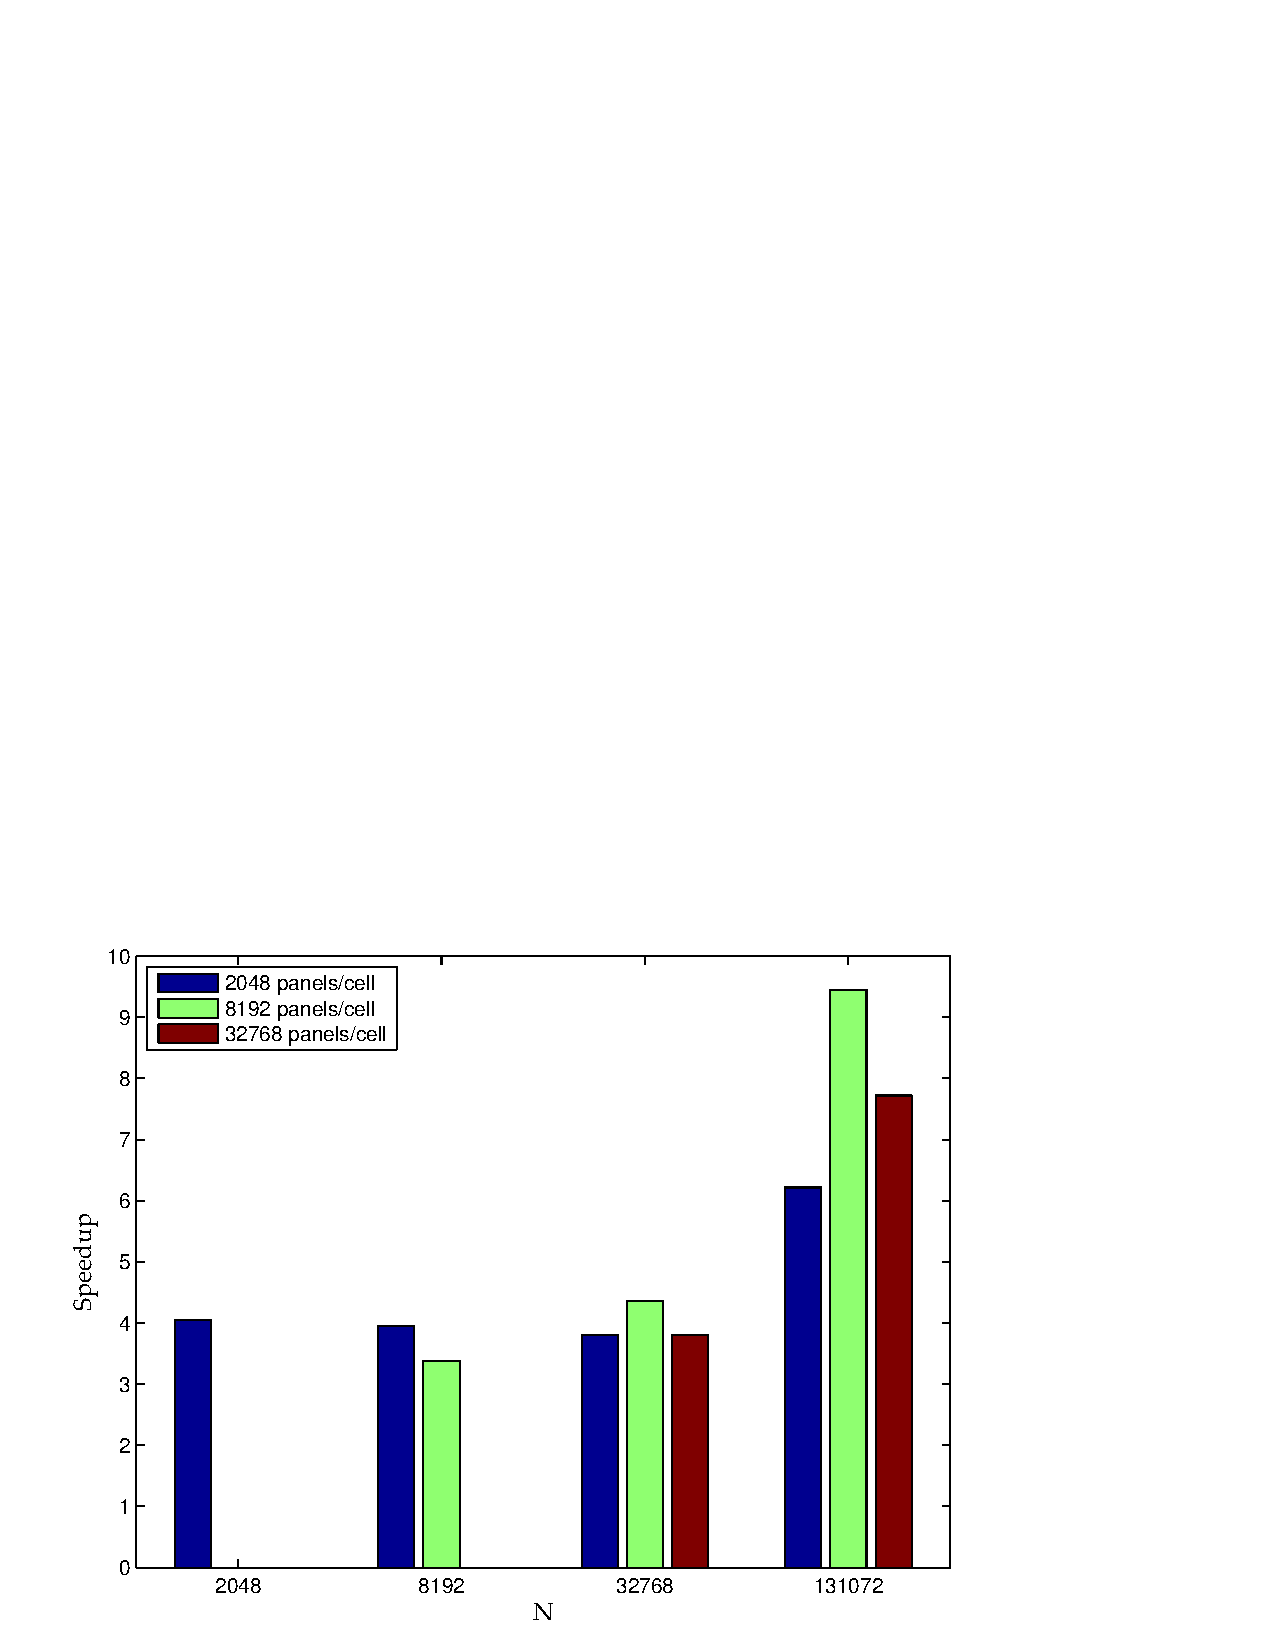
\includegraphics[width=14cm]{img/StokesMultipleCellsSpeedup.pdf}
	\caption{Speedups from multiple ethrocyte tests with varying panels / cell and number of cells. $p = 16$, desired residual $10^{-5}$}
	\label{fig:multiple_cell_speedup}
\end{center}
\end{figure}

Tables \ref{tab:multiple_cell_relaxation_results_2048}-\ref{tab:multiple_cell_relaxation_results_32768} present timing results for both relaxed and non-relaxed solvers for systems involving multiple ethrocytes. The results are also summarized in figure \ref{fig:multiple_cell_speedup}. The first result to note is that the smallest speedup obtained was $3.37\times$, for a single cell of 8192 panels. This shows that even for a relatively small test problem, the speedup due to relaxation is large. Second, for tests where both solvers could utilize the sparse near-field representation, the average speedup is $3.89\times$, a major gain. Finally, we see again that for large problems the memory efficiency of the lower $\ncrit$ for relaxed solves is vital, as for these cases the speedup jumps to between $6-9\times$.

All of these multiple ethrocyte results confirm our expectations from the single cell tests, that we can obtain significant and worthwhile speedups simply from the use of a relaxation scheme and modifying $\ncrit$ to maintain a reasonable balance between {\ptop} and {\mtol} over the course of an iterative solve.

%%%%%%%%%%%%%%%%%%%%%%%%%%%%%%%%%%%%%%%%%%%%%%%
%%%%%%%%%%% PREVIOUS WORK
%%%%%%%%%%%%%%%%%%%%%%%%%%%%%%%%%%%%%%%%%%%%%%%
%\subsection{Comparison with previous work}\label{sec:rbc_previous_comparison}
%
%We have now shown the advantage of relaxation within our own solver for red blood cell problems, so it will be interesting to look at some previous work solving a similar problem, and estimate the benefits that could have been gaining if they had implemented a similar relaxation scheme to ours.
%
%First, we look at the most similar work to ours, using 7500 panels per cell, and 40 cells \cite{Liu2009}. This experiment consisted of 40 cells, each of 7500 panels, giving 300k total panels and 900k degrees of freedom, roughly $2\times$ the size of problem we can currently perform. The value of $\ncrit$ and the exact formulation solved was not given. This system was solved in 730 minutes, taking 49 iterations at $p=15$, solving to a tolerance of $10^{-4}$. We can replicate the majority of these options, although for 40 cells we must use 2048 panels per cell, giving 81920 total panels. This experiment took 33 iterations to converge and 1793s for the fixed-$p$ case, and 639s for the relaxed solver, giving a speedup of $2.80\times$. This speedup is lower than those reported for our experiments due to the change in solver tolerance and thus fewer iterations.

% Other major work in the same field involves a different kind of problem -- using many, less well-resolved cells of a slightly different type, vessicles, in an attempt to simulate something resembling one or more drops of blood. In the first study in this category, $\O{1000}$ panels per cell are used in a time-dependant simulation with up to 600 cells (~600k panels, 1.8m unknowns). This run involved 4500 time steps, in circa 10 days. Remaining details, including the number of iterations required per timestep were not given. 


%%%%%%%%%%%%%%%%%%%%%%%%%%%%%%%%%%%%%%%%%%%%%%%
%%%%%%%%%%% PRECONDITIONERS
%%%%%%%%%%%%%%%%%%%%%%%%%%%%%%%%%%%%%%%%%%%%%%%
\subsection{Preconditioners}\label{sec:rbc_preconditioners}

Even with the results demonstrated in \S\ref{sec:stokes_ethrocyte_relaxation}, the traditional manner of reducing solution time is to use a preconditioner to lower the iteration count, so we must consider the following questions:

\begin{enumerate}
\item Is our relaxation scheme faster than a traditional preconditioned problem solved with fixed $p$?
\item Does our relaxation scheme benefit additionally when used in a preconditioned system?
\end{enumerate}

To find answers to these 2 queries, we perform some experiments on multiple ethrocytes, using the block-diagonal and local preconditioners described in \S\ref{subsec:preconditioners}. As an initial test, we perform a small calculation, with $4$ cells, each of $2048$ panels. This results in a total of $8192$ panels, and a linear system with $24576$ unknowns. This is sizable enough to draw some initial conclusions, yet small enough that it can be performed in $1-2$ minutes in the relaxed case (and $< 5$ minutes with the non-relaxed solver).

Table \ref{tab:relaxation_preconditioning} presents iteration counts and total solution times for both relaxed and non-relaxed solvers for preconditioned and non-preconditioned solvers. In all experiments $\ncrit = 150$ for relaxation, and $\ncrit = 400$ for non-relaxed cases.

\begin{table}[htdp]
\begin{center}
\begin{tabular}{c|c|c|c|c|c|c}

 & \multicolumn{3}{c|}{Relaxed} & \multicolumn{3}{c}{Fixed $p$} \\
 & \multicolumn{3}{c|}{} & \multicolumn{3}{c}{} \\
 Preconditioner & iterations & $\tsolve$ & speedup & iterations & $\tsolve$ & speedup\\
 & & & & & & \\ \hline
  & & & & & &  \\
 Unpreconditioned & 52 & 59.9 & -/- & 52 & 238.0 & -/- \\
 & & & & & & \\
 Block-Diagonal & 45 & 60.8 & 1.18/0.98 & 45 & 212.7 & 1.18/1.13\\
  & & & & & & \\ 
 Local & 37 & 115.8 & 1.54/0.52 & 37 & 241.6 & 1.54/0.99\\
 & & & & & & 
\end{tabular}
\end{center}
\caption{Preconditioning tests for relaxed and non-relaxed solvers -- speedup is in terms of iterations (first value) and $\tsolve$}
\label{tab:relaxation_preconditioning}
\end{table}%

From these results, it is immediately obvious that while the preconditioners increase the rate of convergence, by up to 50\% in the case of the local preconditioner, the time taken for the solve  does not necessarily reflect this decrease in iterations. The block-diagonal preconditioner is the most successful of the preconditioned cases, with a $1.13\times$ speedup in the non-relaxed case (compared to a $1.18\times$ reduction in iterations), however when using relaxation it was slower than not using a preconditioner, albeit to an insignificant degree.

These initial results suggest that while the local preconditioner is effective at increasing the rate of convergence, at this point it cannot be used, as all potential savings from the reduced number of iterations are cancelled out by the cost of performing the inner {\gmres} solve. However, the block-diagonal preconditioner shows promise, working well for the fixed $p$ case, while not providing any benefit in total solve time for the relaxed example.

It must be mentioned here that these preconditioners are working in the \emph{algorithmic} sense, the \emph{implementation} is highly important, and could radically change the current results. Taking the block-diagonal case as an example, we can immediately see the following potential speed-ups:

\begin{enumerate}
\item Explicitly create the inverse of $A_{\text{block}}$ as described in \S\ref{subsec:preconditioners}, changing the application of the preconditioner from a {\gmres} solve (involving 2 matrix-vector products, and multiple other operations) to a single matrix-vector product. Given the nature of $A_{\text{block}}$, $A^{-1}_{\text{block}}$ would require exactly the same amount of storage, while giving a clear speed advantage, at the expense of setup time, due to the cost of inverting many dense matrices of size $\ncrit
\times\ncrit$.

\item Faster sparse matrix operations, notable the matrix-vector product. This could be done in any number of ways, notable examples would be using vectorization (such as {\sse} instructions), or an additional accelerator, for instance a {\gpu}. These options would reduce the cost of applying the preconditioner, while maintaining the reduced iteration count, giving a larger overall speedup.

\end{enumerate}

The implementation of one or both of these suggestions might provide a more useful scheme, but at this point, the fastest time-to solution is for an un-preconditioned solve using a relaxation scheme.

\section{Conclusions}\label{sec:rbc_conclusions}

We have shown compelling results for relaxation schemes in the solution of systems involving Stokes flow around one or more Ethrocytes. These speedups are consistently in the $3-4\times$ range seen in chapter \ref{chapter:stokes}, and are consistent between both the number of ethrocytes used and the level of discretization used per ethrocyte. Further, we have demonstrated that our relaxed solver outperforms a traditionally preconditioned linear system. 

We can also compare this work to the most similar example in literature \cite{Liu2009}. As previously mentioned, 40 non-deformable cells of 7500 panels each were used, giving 300k total panels and 900k degrees of freedom, roughly $2\times$ the size of problem we can currently perform. Most simulation variables were given, with the notable exception of $\ncrit$. The exact formulation of Stokes {\bem} used is not given. This system was solved in 730 minutes, taking 49 iterations at $p=15$, solving to a tolerance of $10^{-4}$. We can replicate the majority of these options, although for 40 cells we must use 2048 panels per cell, giving 81920 total panels. This experiment took 33 iterations to converge and 1793s for the fixed-$p$ case, and 639s for the relaxed solver, giving a speedup of $2.80\times$. While this speedup is lower than those reported for our experiments due to the change in solver tolerance and thus fewer iterations, it would still give an approximated run time of 260 minutes.

The reduction in solution time from an algorithmic change presents an increase in capability for {\fmmbem} methods that should be applicable to a majority of existing codes. The ability to both perform experiments in 1/3 to 1/4 the time allows more test cases to be run, or, potentially, a higher resolution case can be run in the same timeframe. This presents advantages for all use cases -- if time constrained, experiments can be performed much quicker, while if accuracy constrained, higher precision experiments can be performed without the previous cost in computational time.
\cleardoublepage

% -------------------------------------
% CHAPTER 8: CONCLUSIONS
% -------------------------------------
%!TEX root = ../thesis.tex

\chapter{Conclusions}
\label{chapter:conclusions}
\thispagestyle{myheadings}

% set this to the location of the figures for this chapter. it may
% also want to be ../Figures/2_Body/ or something. make sure that
% it has a trailing directory separator (i.e., '/')!
\graphicspath{{Conclusions/}}

\section{Achievements and Findings}

% applied relaxed solver to FMM-BEM
The theory of inexact-Krylov iterations has been applied for the first time for {\fmmbem} problems and verified against standard {\gmres} solvers. It has been tested for both Laplace and Stokes problems and the convergence of the associated linear solves, along with the resulting accuracy of the result has been found to be comparable in all cases. Further, this new method has been applied to the field of the flow of red blood cells (ethrocytes), and has demonstrated significant \emph{algorithmic} performance gains in this engineering example. More detailed conclusions can be summarized as follows.

% verified on simple Laplace problems, explored parameter space
For the simplest test problem explored, experiments using the Laplace equation showed the validity of using a relaxed {\gmres} solver for {\fmmbem}. In all cases, the relaxed solver provided reduced time-to-solution, while maintaining comparable iteration counts, convergence rates and final residuals. In the course of a parameter study involving these equations, we determined the following general rules for the use of a relaxed method:

\begin{itemize}
\item Higher required precisions will result in more significant reductions to time-to-solution, due to the strong scaling with respect to series truncation value, $p$ in the {\fmm}.

\item Problems that require large numbers of iterations in order to reach a satisfactory solution tolerance will benefit more from relaxed schemes -- the nature of {\gmres} results in a large number of iterations requiring comparatively low accuracy from the matrix-vector product; iterations that benefit greatly from relaxation's reduced accuracy requirement.

\item The traditional thinking within the {\fmm} community that the computation time for near and far-fields should be balanced, requires modifications for use within a relaxed solver. As the desired tolerance, and thus required $p$ decreases, the cost of the far-field reduces significantly, while the near-field cost stays constant. Thus, for minimized time-to-solution, the best configuration is to shrink the near-field to the smallest possible whilst retaining accuracy. The higher cost of initial iterations compared to balanced evaluations is made up for by the larger number of low-cost iterations during the remainder of the solve.
\end{itemize}

% verified on tougher Stokes problem, verified speedups
We next used a more difficult problem, creeping or Stokes flow, to test our conclusions from the Laplace experiments, and to show the applicability of the inexact {\gmres} to a tougher, more relevant problem. In all cases, once again, the relaxed solver gave comparable iteration counts and final residuals, while providing significant speedups, in the order of $3-4\times$, for time-to-solution. These experiments also contributed the idea that a \emph{minimum} value of $p$ may need to be set for tough problems, in order to maintain overall accuracy. 

% applied to RBC problem, single & multiple cells, explored speedups
Finally, the insights provided from test problems were applied to a more significant, real-world application, the flow of red blood cells. These experiments demonstrated that for a relevant simulation, the relaxed {\gmres} solver can provide significant reductions in solution time, often by a factor of $4\times$, resulting in huge time savings. As a corollary to the reduced time, the relaxed solver also provides a more memory-efficient method, due to the smaller near-field, and thus reduced memory footprint of the near-field sparse matrix.

% summarise w/bullet points
In summary, the following discoveries were made in this work:
\begin{enumerate}
\item The theory behind inexact Krylov solvers is fully applicable to {\fmmbem} applications, and can provide significant benefits in terms of time-to-solution, while requiring little effort to add to an existing {\fmmbem} code.

\item Based on the accuracy required, and number of iterations required to solve the linear system, we can predict whether a problem will benefit or not from relaxed solvers.

\item Relaxation can be applied successfully to more difficult systems, such as those from the Stokes equations. After these experiments we can say with some confidence that relaxation is likely to work with any equation, as long as accuracy and iteration count requirements are met.

\item There are significant \emph{algorithmic} performance benefits from using a relaxed solver. Speedups obtained from the current implementation for Stokes problems were consistently in the $3-4\times$ range, and due to the algorithmic nature of the improvement, should be comparable for other implementations.
\end{enumerate}

\section{Further Work}

% This thesis has already presented a significant body of work, however there are always more capabilities to be added, and improvements to make. The following suggestions for further work would both increase the number of problems that could be tackled and provide more options for researchers. Due to the algorithmic nature of the improvements presented in the previous chapters, we would expect all of the following to benefit from relaxation schemes, 

\subsection{Distributed-memory Parallelization}

We already have a basic shared-memory parallel evaluator for the {\fmmbem}, however for large problems we run in problems with memory consumption, especially when trying to use the sparse-matrix form of the near-field shown in \S\ref{sec:fmm_near_field}. Moving to a full parallel code would allow us to compute much larger problems due to both the addition of extra computing power, and access to more memory.

\subsection{Hypersingular / Dual Formulation for Stokes}

While we have used a standard, or ``conventional'' formulation for our Stokes {\bem}, it is also possible to reformulate the problem in terms of a Hypersingular {\bem}, so-named for the existence of a new hypersingular operator that appears. This formulation can have problems with the uniqueness of solutions, so  a combination of both conventional and hypersingular formulations was proposed \cite{Liu2009} in order to maintain the better linear system characteristics of the hypersingular form, while retaining a unique solution. This combined approach would change the convergence properties of the {\bem} by reducing the number of iterations, while increasing the amount of work per iteration, and thus potential savings from relaxation, due to the additional operators required. 

\subsection{Higher-Order Elements}

While this thesis concentrates on {\bem} with flat, constant-value triangles, there exist other, higher-order elements. Common examples of these would be flat panels with either linear or quadratic distributions of value across them, or even curved panels. These additions would provide better accuracy with fewer panels for some classes of problems, at the cost of more computational work for the {\ptop} and {\ptom} operators, changing the balance of near and far-field computation for relaxed problems.

\subsection{Linear-Elasticity Equations}

A natural extension of the work on the Stokes equations would be extending to the linear elasticity equations. There already exist formulations of the {\fmm} based around decomposition into harmonic {\fmm}s \cite{fuEtal98}, similar to those for Stokes. Further, the analytical integration routines used in \S\ref{subsubsec:analytical} were originally for linear elasticity, and were modified for our use for Stokes problems. Not only would this be a relatively simple addition to the work, but it would open up whole new application areas, both stand-alone and in conjunction with the red-blood cell work in chapter \ref{chapter:rbc}. In particular, the application of ethrocytes moving and deforming within blood vessels would be enabled with this set of additional {\fmm} kernels.

\subsection{FMM Algorithmic improvements}

As stated in \S\ref{sec:laplace_expansions}, there exist several algorithmic improvements for the Laplace {\fmm} used for all problems in this thesis. These improvements lower the complexity of translation operators from $\O{p^{4}}$ to $\O{p^{3}}$, making the {\fmm} more efficient, especially for high accuracy (high $p$) cases. While we would still expect relaxation schemes to provide a significant benefit to solution times, the balance of near and far-field computations would be likely to change.
\cleardoublepage

\begin{appendices}
% -------------------------------------
% APPENDIX A: FMM_Plan
% -------------------------------------
\newpage
\include{Appendix/FMM_Plan}
\cleardoublepage

\end{appendices}
%==========================================================================%
% Bibliography
\newpage
\singlespace
\bibliographystyle{apalike}

% each subdirectory can have its own BiBTeX file
\bibliography{FastMethods,bem,scicomp,InexactMatVec,Misc,barba,scbib}
\cleardoublepage

%==========================================================================%
% Curriculum Vitae
%!TEX root = ../thesis.tex

\addcontentsline{toc}{chapter}{Curriculum Vitae}

\thispagestyle{empty}

\begin{center}
{\LARGE {\bf CURRICULUM VITAE}}\\
\vspace{0.5in}
{\large {\bf Simon Layton}}
\end{center}

% \setcounter{section}{0}
\setcounter{secnumdepth}{-1}

\section*{Research Interests}

Fast multipole methods ({\fmm}) and fast multipole accelerated Boundary element methods. High- performance computing using heterogenous architectures especially {\nvidia}�s {\cuda} environment. Classical algebraic multigrid for engineering applications, including computational fluid dynamics, most notably immersed boundary techniques. Also interested in sparse linear algebra, notably sparse matrix-matrix products and iterative linear solvers. Further experience in fast multipole and boundary element methods.

\section*{Internships}

\paragraph{May-August 2012 -- DevTech Compute intern, NVIDIA}

Worked on integrating the internal NVAMG library into a large open source scientific code. Work included implementing new features to the library using CUDA and optimizing these codes. Also worked on the interception and analysis of BLAS calls in a major structural analysis code, including work on moving suitable calls to cuBLAS and analyzing and profiling full simulation runs on sample industrial problems.

\paragraph{June-September 2011 -- Emerging Applications intern, NVIDIA}

Worked with Jonathan Cohen on finite-volume methods (1 mo.) and algebraic multigrid ({\amg}) in {\cuda} (remaining time) Work on {\amg} included a complete port of the previous {\cpu} only code from within the group to {\cuda}, testing and verification against the Hypre open-source package.

\section*{Education}

\paragraph{PhD, Mechanical Engineering, Boston University, Expected September 2013}

Thesis: \emph{Fast multipole boundary element methods with inexact Krylov iterations and relaxation strategies} -- Use of fast multipole methods as an inexact matrix-vector product for boundary element methods when solved using Krylov iterative methods. The theory behind inexact matrix-vector products is applied to adaptively control the error produced by the fast multipole method in order to minimize the time to solution for boundary element formulations of example engineering problems involving the Laplace and Stokes equations.

\paragraph{MS, Mechanical Engineering, Boston University, Awarded January 2011}

Concentrations: Computational Fluid Dynamics, Fast Evaluation Algorithms, Heterogenous Computing

\paragraph{BSc, Mathematics and Computer Science, University of Bristol, 2008}

Concentrations: Applied Mathematics, Algorithms, Numerical Methods


\section*{Publications}

\begin{itemize}
\item ``How to obtain efficient GPU kernels: an illustration using FMM \& FGT algorithms'', F. A. Cruz, S. K. Layton, L. A. Barba, \emph{Comput. Phys. Commun.}, Volume 182, Issue 10, p.2084-2098 (2011)
\end{itemize}

\section*{Conference Contributions and Talks}

\begin{itemize}
\item ``Classical algebraic multigrid for CFD with CUDA'', GTC 2012, San Jose, CA

\item ``Classical algebraic multigrid for engineering applications'', {\cuda} Fast Forward, {\nvidia}
Booth, SC �11, Seattle, WA, 14th Nov. 2011

\item ``Classical algebraic multigrid using CUDA'', GPU@BU Workshop, Nov. 8th 2011, Boston University

\item ``cuIBM - a GPU-accelerated immersed boundary method'', S. K. Layton, A. Krishnan, L. A. Barba, International Conference in Parallel CFD, Barcelona, Spain, 16-20 May 2011.

\item ``The parallel Fast Gauss Transform in an heterogenous computing environment'', S. K. Layton, F. A. Cruz, L. A. Barba, US National Congress in Computational Mechanics, USNCCM'09; Columbus, OH, July 2009.
\end{itemize}

\section*{Workshops}

Pan-American Advanced Studies Institute (PASI) - Universidad Santa Maria, Valparaiso, Chile
(January 2011) - Fully funded by NSF

\section*{Fellowships}

\begin{itemize}
\item Dean�s Fellow, Boston University College of Engineering, 2008-2009
\item Graduate Teaching Fellow, Boston University College of Engineering, Fall 2009
\end{itemize}

\section*{Research}

\paragraph{2009-Present} -- Research Assistant at Boston University for Prof. L. Barba, working on heterogenous computing using {\cuda} with varied applications, including fast multipole accelerated boundary element methods, relaxed Krylov solvers, algebraic multigrid, fast evaluation of sums of Gaussians, Computational Fluid dynamics and high order non-oscillatory finite difference schemes for systems of conservation equations.

\paragraph{2008-09} -- Research Assistant at Boston University for Prof. L. Barba, working on fast evaluation of Gaussians and heterogenous computing using {\cuda}.

\paragraph{2007-08} -- 9 month final mathematics research project with Prof. L. Barba: ``Implementation and numerical experimentation of fast algorithms for particle methods with Gaussians''

\section*{Teaching}

\paragraph{2009}
Teaching assistant for Fluid Mechanic course, ME303, Boston University

\section*{Skills and Qualifications}

\begin{itemize}
\item Use and administration of Linux, Mac OS X, Microsoft Windows systems
\item Programming in C, C++, CUDA, Python, bash, Java, Matlab, Mathematica
\item Use of Boost, OpenMP, MPI, Cusp, Thrust and varied other software libraries
\item Familiar with CFD packages such as OpenFOAM and Gerris
\end{itemize}�
 

%==========================================================================%
\end{document}
